\documentclass{ucetd}
\usepackage{subfigure,epsfig,amsfonts}
\usepackage[sort&compress,numbers]{natbib}
\usepackage{amsmath}
\usepackage{bm}
\usepackage{amssymb}
\usepackage{amsthm}
\usepackage{braket}
\usepackage{mathrsfs}
% \usepackage{cancel}
\usepackage{tabularx}
% Following 2 lines silence the \underline warnings.
\usepackage{silence}
\WarningFilter{latex}{Command}
\DeclareMathOperator{\sinc}{sinc}
\usepackage{sectsty}
\usepackage{float}
\usepackage{graphicx}
\usepackage{color,soul}
\usepackage{lipsum}
\usepackage{emoji}
%Modify directory for loading graphics
\graphicspath{{Figures/}}
%Extra
\usepackage{bm}
\usepackage{braket}
\usepackage{setspace}
\usepackage{listings}
\usepackage{multicol}
\usepackage{verbatim}
\usepackage{physics}
\usepackage{dsfont}
\usepackage{pdflscape}
\usepackage{adjustbox}
\usepackage{blkarray}
\usepackage{colortbl}
\usepackage{hyperref}
% \usepackage{rotating}
\newcommand{\dg}{$^{\circ}$} 
\usepackage{lipsum}% http://ctan.org/pkg/lipsum
\newsavebox{\myimage}
\usepackage{graphicx}
\usepackage{fancyhdr}
\usepackage{kantlipsum}
\usepackage{afterpage}
\usepackage{pdflscape}
\usepackage{multirow}
\newcolumntype{C}[1]{>{\centering\arraybackslash}m{#1}}

\renewcommand{\bibname}{References}

%% Use these commands to set biographic information for the title page:
\title{Optical Design and Analysis of Next Generation Instruments for Measurements of the Cosmic Microwave Background
}
\author{Grace E. Chesmore}
\department{Department of Physics}
\division{Physical Sciences Division}
\degree{Doctor of Philosophy}
\date{Month and Year of Graduation}  % date of degree awarding, not the date of the defense

%% Use these commands to set a dedication and epigraph text
% \dedication{Dedication text}
% deducation text 
\epigraph{}
\usepackage{caption}
%\captionsetup{font=footnotesize}
\usepackage{pdfpages}

\begin{document}

\maketitle

\makecopyright
% \makededication
% \makeepigraph

%% Make the various tables of contents
\tableofcontents
\cleardoublepage
\phantomsection
\listoffigures
\cleardoublepage
\phantomsection
\listoftables
\newpage

\begin{center}
    \textit{This thesis represents the motivations, results, and conclusions from the following works}:
    \\
    \begin{enumerate}
        \item[\cite{act_ptsrc}] \textit{The Atacama Cosmology Telescope: Beam Estimation for DR6 with Point Source Stacking}. G. E. Chesmore, et al. in progress.
        \item[\cite{chesmore2022}] \textit{The Simons Observatory: Characterizing the Large Aperture Telescope Receiver with Radio Holography}. G. E. Chesmore, et al. Applied Optics, 2022.
        \item[\cite{Chesmore:21}] \textit{The Simons Observatory: HoloSim-ML: machine learning applied to the efficient analysis of radio holography measurements of complex optical systems}. G. E. Chesmore, et al. Applied Optics, 2021.
        \item[\cite{Xu_2021}] \textit{The Simons Observatory: Metamaterial Microwave Absorber (MMA) and its Cryogenic Applications}. Z. Xu, G. E. Chesmore, et al. Applied Optics, 2021.
        \item[\cite{ches18}] \textit{Reflectometry Measurements of the Loss Tangent in Silicon at Millimeter Wavelengths}. G. E. Chesmore, et al. Proceedings from the 8th ESA Workshop on Millimetre-Wave Technology and Applications, 2018.
    \end{enumerate}

\end{center}
\newpage

\abstract
The Cosmic Microwave Background (CMB) carries the imprints of the conditions in the early universe and the large-scale structure it has traversed as it travels to our telescopes. This radiation from the early universe serves as a window into the physics of our universe. From the CMB, we can study primordial gravitational waves, large scale structure formation, sum of neutrino masses, dark energy, dark matter, and fundamental physics. Achieving these ambitious science goals requires equally ambitious instrumentation.
CMB-S4 and ongoing stage 3 ground-based CMB experiments are designed to observe the CMB temperature and polarization signals to an unprecedented sensitivity. A combination of three Large Aperture Telescopes (LATs) and eighteen Small Aperture Telescopes (SATs) will measure the temperature and polarization anisotropy of the CMB with $\approx$500,000 background noise-limited detectors operating at $\approx$100\,mK, covering frequencies from $\approx$20 to $\approx$300\,GHz.

In order to measure the tiniest signals of the CMB, we must control optical systematics and advance detector sensitivity to unprecedented levels. I will discuss the techniques to control optical systematics, design highly sensitive detectors and feedhorn arrays, and characterize their performance. Using a holography imaging setup as a beam mapper, I will evaluate the performance of the optical properties of novel absorbers I developed, and beam map a complete cryogenic optical system. I developed software to model these systems,  including hardware imperfections, demonstrating how systematics propagate into measurements; the software also uses machine learning to correct such systematic errors by correcting alignment of mirrors.  Lastly, I will present a novel approach for characterizing the on-sky beam with maps from Atacama Cosmology Telescope Data Release 6.  Understanding the beam of the instrument is critical for characterizing the angular response of the instrument, and therefore critical for achieving the ambitious science goals in ACT and beyond.  I will present how stacking point sources from existing CMB maps, to determine the instrument beam, compares to the existing method of mapping planets.

\mainmatter

% Chapter 1

\chapter{Introduction} % Main chapter title

\label{ch:intro} % For referencing the chapter elsewhere, use \ref{Chapter1} 

%----------------------------------------------------------------------------------------

% Define some commands to keep the formatting separated from the content 
\newcommand{\keyword}[1]{\textbf{#1}}
\newcommand{\tabhead}[1]{\textbf{#1}}
\newcommand{\code}[1]{\texttt{#1}}
\newcommand{\file}[1]{\texttt{\bfseries#1}}
\newcommand{\option}[1]{\texttt{\itshape#1}}
% \newcommand{\enquote}[1]{``#1"}
%----------------------------------------------------------------------------------------

In 1965 at Bell Labs, Arno Penzias and Robert Wilson serendipitously detected ``noise" with their microwave antenna.  This noise was isotropic (same in all directions) and homogenous (same in all locations), and was ultimately the measurement of the Cosmic Microwave Background; radiation from the early universe.
\begin{equation}
    I(\nu,T) = \frac{2h\nu^2}{c^2}\frac{1}{e^{\frac{h\nu}{k_B T}} -1}
    \label{eq:blackbody}
\end{equation}
The temperature spectrum of the Cosmic Microwave Background (CMB) was measured to be a near-perfect black-body (Eq.~\ref{eq:blackbody}), with a mean temperature of~\cite{burke_graham-smith_wilkinson_2019}:
\begin{equation}
    T_{\text{CMB}} = 2.725\,K
\end{equation}
The spectrum lies in the infra-red range of the electromagnetic spectrum, and peaks at a wavelength $\lambda = 1.5\,\text{mm}$ (Figure~\ref{fig:cobe_power_spectra}). 

This near-perfect black-body is understood to originate during the early universe by the rapid collision of photons with free electrons (Thompson scattering), to keep radiation in thermal equilibrium with hot dense matter.  As the universe expanded and cooled, however, this spectrum kept its same form~\cite{weinberg_cosmo}.  Because it formed during the early universe, the CMB is a backlight into not only early universe properties, but also late universe physics such as large-scale structure and dark matter.  The CMB, therefore, carries a wealth of information about the fundamental physics of our universe.

\begin{figure}[t]
    \centering
    \includegraphics[width = \textwidth]{Figures/cobe_power_spec.pdf}
    \caption{Left: Spectrum of the CMB from the COBE satellite~\cite{1994ApJ...420..439M}.  The deviation from an ideal blackbody is magnified $\times\,400$ in the bottom panel.  Right: First-year maps from the COBE Differential Microwave Radiometer in 1992~\cite{1992ApJ...396L...1S}.}
    \label{fig:cobe_power_spectra}
\end{figure}

\section{The Expanding Universe}
The evolution of the universe can be described using an extension of Einstein's equations.  To measure distances in an expanding universe, we employ the metric $ds$, which depends on the curvature of the space, with curvature $\kappa$:
\begin{equation}
    ds^2 = -c^2dt^2 + a(t)^2[dr^2 + S_\kappa (r^2)d\Omega^2]\text{ ,}
\end{equation}
where
\begin{equation}
    d\Omega^2\equiv d\theta^2 + \sin^2\theta d\phi^2
\end{equation}
and
\begin{equation}
    S_\kappa(r) = \begin{cases} R\sin(r/R) & (\kappa = +1) \\
  r & (\kappa = 0) \\
   R\sinh(r/R) & (\kappa = -1)\end{cases}
\end{equation}
Here, we consider the scale of the universe as a function of time $a(t)$, which relates to the redshift $z$ as
\begin{equation}
    a(t) = \frac{1}{a+z}\text{ ,}
\end{equation}
where we set today's $a=1$.  If $a(t)$ is increasing, then the object is ``red-shifted", or a decrease in frequency.  This relationship can be expanded for nearby sources:
\begin{equation}
    a(t)\approx a(t_0)[1+(t-t_0)H_0+ \ldots ]
\end{equation}
where we've introduced the Hubble Constant $H_0$.  The Hubble Constant quantifies the expansion of our universe:
\begin{equation}
    H_0\equiv \bigg(\frac{\dot{a}}{a}\bigg )_{t=t_0}\; .
\end{equation}
In recent decades, astronomers and cosmologists have worked to determine the exact value of $H_0$ using both early- and late-universe physics.  As the two methods return differing values of the Hubble Constant, this field continues to evolve with new statistical methods and precision instrumentation.

\section{The Three Equations of the Universe}
The dynamics of the universe are neatly described by three equations, which connect its curvature to the energy density $\rho$ and pressure $P$.

\noindent
\textbf{Friedmann Equation}:  Stemming from Einstein's relativistic field equations, the Friedmann equation describes a homogenous and isotropic universe:  
\begin{equation}
    \bigg ( \frac{\Dot{a}}{a} \bigg ) = \frac{8\pi G}{3c^2}\rho(t) - \frac{\kappa c^2}{R_0}\frac{1}{a(t)}
\end{equation}
where $\rho$ is the energy density, $G$ is the gravitational constant, $c$ is the speed of light, $\kappa$ is the curvature parameter, and $R_0$ is the radius of curvature at present time $t=0$.  The energy density is evolving, and made up of matter ($\rho_m=\rho_{m0}a^{-3}$), radiation ($\rho_r=\rho_{r0}a^{-4}$), and a cosmological constant ($\rho_{\Lambda}=\rho_{\Lambda 0}$), thus the Friedman equation takes the form:
\begin{equation}
    \frac{H^2}{H_0^2} = \frac{\Omega_{r0}}{a^4} + \frac{\Omega_{m0}}{a^3} + \Omega_{\Lambda 0} + \frac{1-\Omega_0}{a^2}
\end{equation}
where we normalize the energy density $\rho$ by the critical density $\rho_c(t)$, where $\rho_c(t) = \frac{3c^2}{8\pi G}$~\cite{ryden_2016}.  This results in the new variable:
\begin{equation}
    \Omega(t) = \frac{\rho(t)}{\rho_c(t)}
\end{equation}
Today, cosmologists assume a standard model of cosmology, which is referred to as the ``$\Lambda$CDM model".  The $\Lambda$CDM model assumes a flat $\Omega(t)=1$ universe, consisted mostly of baryonic ($\Omega_b h^2$) and cold dark matter ($\Omega_c h^2$) densities.  We will discuss this model further in the next sections.

\noindent
\textbf{Fluid Equation}:  Energy conservation can also be applied to describe the dynamics of the universe through the first law of thermodynamics (Eq.~\ref{eq:thermo1}).  This implies the sum of gravitational potential and kinetic energy of expansion is conserved~\cite{ryden_2016}.
\begin{equation}
    dQ = dE + PdV
    \label{eq:thermo1}
\end{equation}
\begin{equation}
    \dot{\rho} + \frac{3\dot{a}}{a}(\rho + P) = 0
    \label{eq:fluid_universe}
\end{equation}
\noindent
Solving the fluid equation (with $P=w\rho$) yields the equation of state:
\begin{equation}
    \rho \propto a^{-3(1+w)}
\end{equation}
with the time-independent $w$~\cite{weinberg_cosmo}.  For example, in the case of a cold matter dominated universe (e.g. dust, $P = 0$) $\rho\propto a^{-3}$, and in a hot matter universe (e.g. radiation, $P=\rho/3$) $\rho\propto a^{-4}$.

\noindent
\textbf{Acceleration Equation}: Combining the first two equations, which constrain an energy conserved universe, yields the acceleration equation describing how our universe expands over time.  
\begin{equation}
    \frac{\ddot{a}}{a} = - \frac{4\pi G}{3 c^2} (\rho + 3 P)
\end{equation}
\begin{figure}
    \centering
    \includegraphics[width=\textwidth]{Figures/universe.pdf}
    \caption{The history of the universe as we understand it today.  After the Big Bang, the CMB is emitted during the Recombination era at around 380,000.  The photons emitted then traversed large-scale structure to get to our detectors, and therefore we can study late universe large-scale structure through measurements of the CMB.  Credit: ESA/Planck Team~\cite{NASApic}, re-touched by Chesmore.}
    \label{fig:universe_timeline}
\end{figure}
\section{The Case for Cosmic Inflation}
Three pillars provide evidence for the Big Bang Theory, whereupon our universe came into existence.

\noindent
\textbf{The Expanding Universe}: As we've previously discussed in this chapter, the universe is predicted to be currently expanding.  This has been studied and proven by observations of late-universe objects like galaxies~\cite{1999ApJ...517..565P}.  By measuring the velocity and distance of an object, scientists determined (using the Hubble Law) objects in the past were closer together, and today are farther apart.  

\noindent
\textbf{The Cosmic Microwave Background}:
Radiation from a source of known temperature is described by a black-body spectrum.  We've introduced the CMB as radiation from the early universe.  We've also introduced the CMB as a blackbody spectrum.  It can be shown that, in an expanding universe, the blackbody will maintain its shape, its temperature will decrease as the wavelength shifts lower.  Therefore, the CMB serves as evidence of a dense hot radiation source before the universe expanded, with a consistent black-body shape.

\noindent
\textbf{Abundance of Light Elements}:  Such an abundance of light elements in today's universe suggests a hot, dense beginning to the universe.  As the universe cooled and expanded, light particles formed by a fusion process called Big Bang Nucleosynthesis (BBN).  The amount of light particles measured today are in agreement with predictions made by BBN.

These three pillars indicate a valid understanding of cosmology, but this cosmology remains incomplete.  Problems which remain are listed below.  The theory of inflation has the potential to explain the mentioned puzzles.

\begin{enumerate}
    \item Flatness problem:  Measurements of the observable universe present a nearly flat spatial geometry ($\Omega_{\text{total}}=1$).  This would imply a flat geometry at the initial moments of our universe as well.  But for what reason would the universe begin with a flat geometry?  Inflation answers this by suggesting our universe might have curvature, but this rapid expansion blows up any curvature such that the tiny amount we can observe appears flat. 
    \item Horizon problem:  The sky appears remarkably (and statistically) uniform in all directions.  The CMB confirms this, as we measure this radiation to be uniform to one part in $100,000$.  The particle horizon distance is only $2^{\circ}$, so how could the entire sky be so nearly uniform?  Inflation solves this because such an accelerated expansion creates a paradigm where all the observed sky has a chance to come into causal contact.
    \item Magnetic monopole problem:  Magnetic monopoles are analogous to electrons, which would emit a magnetic charge.  However, we have never measured a single monopole in our universe, nor do we know that they exist.  Meanwhile, the Grand Unified Theory (GUT) predicts an extremely low density of magnetic monopoles; GUT predicts one monopole per Hubble radius.  Inflation solves this by diluting the expected number of monopoles thus explaining why we have not measured a single one.
\end{enumerate}
\section{$\Lambda$CDM Cosmology}
Today, the universe is described by the $\Lambda$CDM model, which assumes a flat universe ($\Omega_{\text{tot}}=1$) which is expanding at an accelerating rate, and is dominated by cold dark energy and cold dark matter.  Further, the $\Lambda$CDM model assumes dark energy taking the form of a cosmological constant $\Lambda$, which is expressed as a constant energy density:
\begin{equation}
    \rho_\Lambda = \frac{c^2}{8\pi G}\Lambda 
\end{equation}
The $\Lambda$CDM model neatly models the universe in six parameters: the baryonic density $\Omega_b\,h^2$, the cold dark matter density $\Omega_c\,h^2$, $\ln(10^{10}A_s)$, the spectral index of inflation $n_s$, the size of the acoustic horizon at decoupling 100\,$\theta_{*}$, and the reionization optical depth $\tau$.  Further, the standard model assumes a constant number of neutrino $N_{\text{eff}}$ and sum of neutrino masses $\Sigma m_\nu$. The most up-to-date values are listed in Table~\ref{tab:cosmology_recent_results}.  All of these parameters impact the shape of the CMB spectra which we measure today.

\section{The CMB Temperature Power Spectra}
The Cosmic Microwave Background carries rich science in its temperature and polarization spectra.  The CMB temperature spectrum can be decomposed into spherical harmonics, which result in power spectra as a function of multipole moment $\ell$, where $\ell\approx180/\theta$ and $\theta$ is angular scale on the sky.  The temperature fluctuations of the CMB are decomposed into spherical harmonics:
\begin{equation}
\frac{\delta T}{T}(\theta,\phi) = \sum_{\ell=2}^{\infty} \sum_{m=-\ell}^{\ell} a_{\ell m} Y_{\ell m}(\theta,\phi)
    \label{eq:cmb_temp}
\end{equation}

where $\ell$ and $m$ are multipoles of the spherical harmonic $Y_{\ell m}$, $a_{\ell m}$ are expansion coefficients, and $\theta$ and $\phi$ represent the angular position on the sky.  You'll notice the first summation of Equation~\ref{eq:cmb_temp} begins at $\ell=2$ rather than $\ell=0$; the $\ell=1$ coefficient corresponds to the earth's motion with respect to the CMB, and the $\ell=0$ coefficient is the mean temperature of the CMB, so we neglect those terms.  The coefficients $a_{\ell m}$ are independent variables, and relate to the CMB's angular power spectra via:
\begin{equation}
    C_\ell^{TT} = \frac{1}{2\ell +1} \sum_{m=-\ell}^{m=\ell} |a_{\ell m}|^2
\end{equation}

This is the temperature power spectrum of the CMB.  Figure~\ref{fig:measured_cmb_spec} shows the measured CMB temperature power spectrum from the Atacama Cosmology Telescope, the South Pole Telescope, and WMAP~\cite{Das_2014}.
\begin{figure}[t]
    \centering
    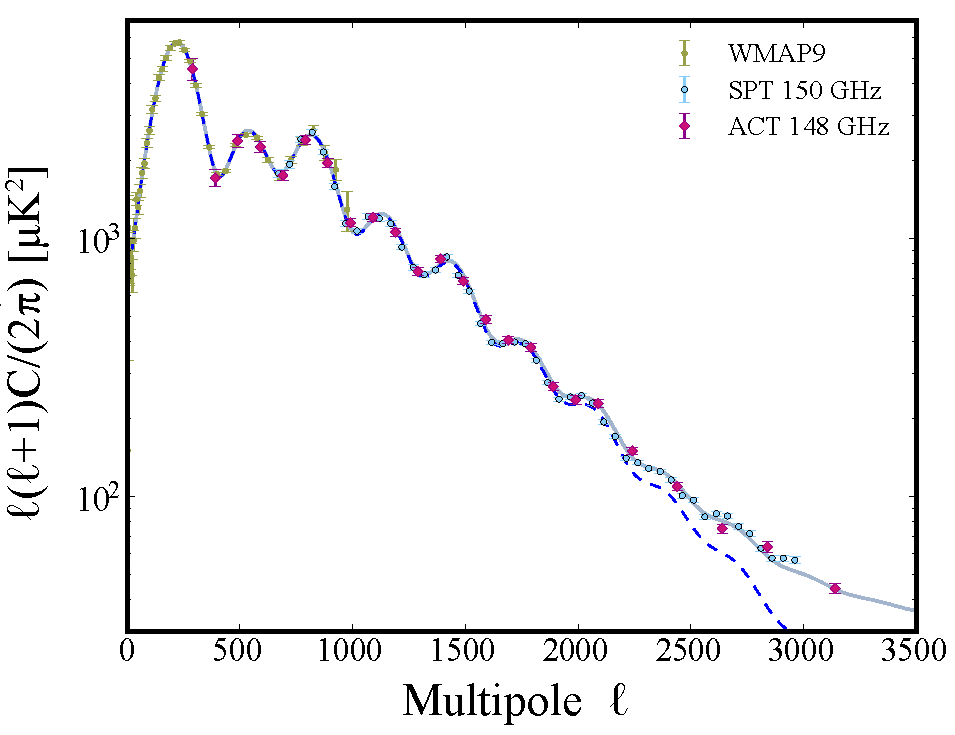
\includegraphics[width = .8\textwidth]{Figures/temp_power_spectrum.pdf}
    \caption{The CMB temperature power spectra measured by WMAP (yellow), the South Pole Telescope (blue) and the Atacama Cosmology Telescope (purple)~\cite{Das_2014}.  The temperature anisotropies of the CMB will be measured with the Simons Observatory and CMB-S4, two upcoming cosmology experiments, with further precision.}
    \label{fig:measured_cmb_spec}
\end{figure}

The shape of the CMB power spectra unlocks properties of the early universe.  For example, the first peak in the power spectrum at around $\ell\approx220$ corresponds to the angle at which we observe the sound horizon, or the distance that sound can travel between the big bang and recombination.  The measurement of this power spectrum's morphology can also determine physical matter and baryon densities.  The dark energy properties of our universe can be constrained by the power spectrum peak, as the dark energy and matter densities jointly alter the distance to last scattering~\cite{Hadzhiyska_2019}.  The matter denstiy of the universe alters the expansion of the universe, which determines when the universe reaches the temperature of last scattering, or when photons begin to stream freely.  The smaller angular scale distortions are in part due to an inhomogeneous universe at the time of last scattering ($z\approx 1100$).  

\section{The Polarized CMB}

The CMB is predicted to be polarized, due to Thompson scattering by free electrons during the era of recombination~\cite{weinberg_cosmo,Page_2007}.  Measuring this polarization would indicate the beginning of reionization and further have the potential to uncover primordial gravitational waves.  Just as the CMB's temperature spectrum is decomposed in spherical harmonics, we also decompose the polarized components.  We refer to the CMB's polarization signals as ``E-modes" and ``B-modes" after their likeness to curl-free (electric) and divergence-free (magnetic) fields (Figure~\ref{fig:e_b_pol}).
\begin{figure}
    \centering
    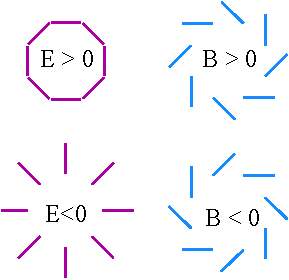
\includegraphics[width = .45\textwidth]{Figures/EB_pol.pdf}
    \caption{The polarization modes of the CMB.  The E modes have no curl, while the B modes have no divergence.  The polarization pattern in the CMB is caused by...}
    \label{fig:e_b_pol}
\end{figure}

The E-modes are produced by the density perturbations via Thompson scattering from a local quadrupole.  For this reason, the EE spectra peaks when scattering is highest, and when velocity is highest, between the two temperature spectrum peaks.  Primordial gravitational waves produce B-modes through Thompson scattering.  Further, the large-scale structure gravitationally lenses CMB photons traveling through, adding to the B-mode polarization spectra.  The scalar-to-tensor ratio, $r$, is directly determined through measurements of the B-mode polarization, as scalar perturbations generate E-mode polarization.

Let's now define the polarization signal basis of E- and B-modes.  The electric field of a photon travelling in the $\hat{z}$-direction is described by
\begin{equation}
    \Vec{E} = (E_x\hat{x} + E_y\hat{y})e^{i k_z - \omega t } \text{ .}
    \label{eq:e_photon}
\end{equation}
The Stokes parameters make up the basis of a photon's polarization, which is obtained from the electric field $\Vec{E}$, with parameters: intensity $I$, linear polarization $Q$, diagonal polarization $U$, and circular polarization $V$ (Eq.~\ref{eq:e_photon} and Eq.~\ref{eq:stokes}).

\begin{equation}
\begin{split}
    I & = |E_x|^2 + |E_y|^2 \\
    Q & = |E_x|^2 - |E_y|^2 \\
    U & = E_x E_y^* + E_x^*E_y\\
    V & = i(E_x E_y^* - E_x^*E_y) \\
\end{split}
\label{eq:stokes}
\end{equation}

The CMB should not carry any circular polarization, but can occur due to secondary mechanisms which take place after the surface of last scattering.  Just as the temperature power spectrum is decomposed into spherical harmonics, we express the polarization of the CMB in terms of spin-2 (where $a^*_{-2,\ell m} = a_{2,\ell m}$) spherical harmonics:
\begin{equation}
(Q \pm iU) = \sum_{\ell m}^{\pm 2} a^{\pm 2}_{\ell ,m} Y_{\pm2,\ell m} \text{ ,}
\end{equation}
where the expansion coefficients $a_{\ell m }^E$ and $a_{\ell m }^B$ are defined as
\begin{equation}
\begin{split}
    a_{\ell m }^E & = -\frac{1}{2}(a_{\ell m}^2 + a_{\ell m}^{-2}) \\
    a_{\ell m }^B & = \frac{i}{2}(a_{\ell m}^2 - a_{\ell m}^{-2}) \text{ .}
\end{split}
\end{equation}
The E- and B-modes of the CMB are then defined as
\begin{equation}
\begin{split}
    E(\theta,\phi) & = \sum_{\ell m} a_{\ell m }^E Y_{\ell m}(\theta,\phi) \\
    B(\theta,\phi) & = \sum_{\ell m} a_{\ell m }^B Y_{\ell m}(\theta,\phi) \text{ .}
\end{split}
\end{equation}
It follows that the CMB's polarized spectra are then defined as
\begin{equation}
    C_{\ell}^{XY} = \frac{1}{2\ell+1}\sum_m \langle a_{\ell m}^{X} a_{\ell m}^{Y*} \rangle 
\end{equation}
Here, $X$ and $Y$ can either be E-mode, B-mode, or temperature T spectra of the CMB, indicating cross-correlated spectra.

\section{Why Care About Beams?}
Every camera has a ``beam" (or optical response) which determines the optical performance (how your picture will turn out).  The smaller your beam, the higher the resolution of your picture.   The Field-of-View (FOV) determines how wide your picture can be.  The noise of your camera's detector determines how grainy the picture comes out.  All of these optical properties are defined by the camera's beam.  To take a picture of the CMB, the telescope is our camera; the beam of the instrument determines the optical performance at a given angular scale.  

This not only affects the immediate quality of our CMB maps, but also impacts the ability to study cosmological science.  Let's consider two cosmological parameters: the spectral index of inflation $n_{s}$, and the number of relativistic species $N_{\text{eff}}$.  The spectral index of inflation $n_{s}$ describes how fluctuations vary with angular scale.  Figure~\ref{fig:cmb_ns} shows the CMB power spectra at three different values of $n_{s}$ and at two different values of $N_{\text{eff}}$.
The red curve plots the achieved sensitivty of Planck for determining the spectral index $n_\text{s}$ and $N_{\text{eff}}$, showing $n_s\pm\sigma_{n_s}$, and $N_{\text{eff}}\pm\sigma_{N_{\text{eff}}}$.  The science goals of SO are plotted in blue to show the increase in sensitivity compared to Planck.  The right-most plot then shows that a mischaracterization of the instrument's beam can mimic the aforementioned uncertainties.  At small angular scales (large $\ell$ values), slight variations of $n_{s}$ change the slope of the power spectrum (Figure~\ref{fig:cmb_ns}).  For this reason, the beam must be well understood and characterized to achieve such ambitious science goals.

\begin{figure}[t!]
    \centering
    \includegraphics[width = \textwidth]{Figures/beam_neff.pdf}
    \caption{The simulated CMB power spectrum at varying spectral index of inflation $n_\text{s}$, and varying relativistic species $N_{\text{eff}}$.  Simulations are made with CAMB~\cite{camb_online} and show the $TT$ spectrum's deviation from nominal values, with $n_s\pm\sigma_{n_s}$, and $N_{\text{eff}}\pm\sigma_{N_{\text{eff}}}$.  In red is the sensitivity achieved by Planck, and in blue is the sensitivity goal of Simons Observatory.  The right-most panel simulates a mischaracterized instrument beam and how it can mimic deviations in the $TT$ spectrum of the CMB.}
    \label{fig:cmb_ns}
\end{figure}

Entire classes of inflationary models can be ruled out by constraining $n_{s}$.  Achieving this goal, however, requires precise beam calibration on these small angular scales.  Further, characterizing the polarization leakage from the telescope's beam is critical to map the tiniest signals of the CMB's polarization.  For this reason, this work focuses on beam calibration, both for the Simons Observatory and the Atacama Cosmology Telescope.

\section{Status of the Field}
\begin{table}[b!]
    \centering
    \begin{tabular}{|c|c|c|}\hline 
         Parameter & Planck 2018 Release & ACT 2020 Release \\ \hline
         $100\,\Omega_b h^2$ &  2.241$\pm$0.015 &2.153$\pm$0.030 \\
         $100\,\Omega_c h^2$ & 11.97$\pm$0.14 & 11.78$\pm$ 0.38\\
         $\ln(10^{10}A_s)$ &3.040$\pm$0.016& 3.050$\pm$0.030\\
         $\Omega_\Lambda$ & 0.687$\pm$0.008 & 0.696$\pm$0.022\\
         $n_{s}$ & 0.967$\pm$0.004 & 1.008$\pm$0.005\\
         $100\,\theta_{*}$ & 1.0410$\pm$0.00046 &1.0425$\pm$0.0007 \\
         $\tau$  &0.052$\pm$0.008 &0.065$\pm$0.014 \\
         $t_0$& 13.791$\pm$0.025 & 13.832$\pm$0.047\\
         \hline
    \end{tabular}
    \caption{The most recent cosmological parameters as from the 2018 Planck release~\cite{planck2020} and the 2020 ACT release~\cite{aiola_2020}.  Baryonic and cold dark matter densities $\Omega_b$, $\Omega_c$, dark energy density $\Omega_\Lambda$ spectral index of inflation $n_{s}$, acoustic horizon at decoupling $\theta_*$, reionization depth $\tau$, and the age of the Universe in Gyr, $t_0$.}
    \label{tab:cosmology_recent_results}
\end{table}

Since the detection by Penzias and Wilson in 1965, the cosmology community has made leaps to constrain the black-body of the CMB.  The Cosmic Background Explorer (COBE) was the first to measure the CMB power spectrum from space.  Since COBE, the measurement of fluctuations in the CMB has increased in precision, with experiments like WMAP, Planck, for example.  The South Pole Telescope and the Atacama Cosmology Telescope, two ground-based telescopes, have pushed the measurement further with increased resolution mapping of the sky.

In the coming years, cosmologists aim to detect the tiniest signals of the polarized CMB.  An ongoing challenge in cosmology instrumentation has been characterizing the polarization spectra of the CMB.  Specifically, the B-mode polarization of the CMB offers a unique window into early-universe physics~\cite{weinberg_cosmo}.  Because scalar perturbations generate E-mode polarization, a measurement of the B-mode polarization directly quantifies the scalar-to-tensor ratio, $r$.  The BB-power spectra has been reported by the Polarbear, South Pole Telescope and ACTPol collaborations~\cite{planck_data,choi_2020,PARAde_2014}.

\section{Outline of Thesis}

First, I overview two ground-based cosmology experiments in Chapter~\ref{ch:instruments}: the Atacama Cosmology Telescope (ACT) and the Simons Observatory (SO).  This work focuses on the development and characterization of optical components for the SO.  In the final chapter of this work, I characterize the optical performance of ACT.

In Chapter~\ref{ch:mma}, I present an overview of the meta-material absorbers used in the SO Large Aperture Telescope optics tubes to control stray light.  I also present the characterization of their optical properties using a radio holography receiver.  These tiles are comprised of an outer metamaterial layer, which approximates a lossy gradient index anti-reflection coating. They are fabricated via injection molding commercially-available carbon-loaded polyurethane (25\% by mass). The injection molding technology enables mass production at low cost.  Room temperature optical measurements verify their control of reflectance to less than 1\% up to 65$^{\circ}$ angles of incidence, and control of wide angle scattering below 0.01\%.

The characterization of optical components is continued in Chapter~\ref{ch:si}, where I characterize the reflectivity and loss tangent measured in the W-band (80-125\,GHz) and D-band (125-180\,GHz) in two samples of float zone silicon with intrinsic stoichiometry - one irradiated by neutrons, which increases the resistivity by introducing crystalline defects, and the other unperturbed.  I find the loss tangent $\tan\delta$ of $2.8\times10^{-4}$ and $1.5\times10^{-5}$ for neutron-irradiated silicon and intrinsic silicon, respectively, both with an index of refraction of 3.41.  The results demonstrate the applicability of silicon as a warm optical component in millimeter-wave receivers.  The depth of the reflection nulls provides a sensitive measurement of dielectric losses.

In Chapter~\ref{ch:ot_holo}, I present near-field radio holography measurements of the SO LATR optics.  These measurements demonstrate that radio holography of complex millimeter-wave optical systems comprising cryogenic lenses, filters, and feed horns can provide detailed characterization of wave propagation before deployment.  I used the measured amplitude and phase, at 4\,K, of the receiver near-field beam pattern to predict two key performance parameters: 1) the amount of scattered light that will spill past the telescope to 300\,K and 2) the beam pattern expected from the receiver when fielded on the telescope.  These cryogenic measurements informed the removal of a filter, which led to improved optical efficiency and reduced side-lobes at the exit of the receiver.  This is the first time such parameters have been confirmed in the lab prior to deployment of a new receiver.

Chapter~\ref{ch:sat_holo} presents additional near-field radio holography measurements, this time on the Small Aperture Telescope (SAT) optics tube.  Using the identical holography setup as described in Chapter~\ref{ch:ot_holo}, I present preliminary characterization of the SAT's optical performance; more specifically, I predict two key performance parameters: 1) the beam profile in the near-field and 2) the far-field beam pattern of the telescope expected from the receiver.

Chapter~\ref{ch:holosim} presents Holosim-ML: a Python code for beam simulation and analysis of radio holography data from complex optical systems.  This code uses machine learning to efficiently determine the position of hundreds of mirror adjusters on multiple mirrors with few micrometer accuracy.  I apply this approach to the example of the SO 6\,m telescope.  The ML framework makes the analysis of these measurements from many receiver positions straightforward to analyze.  I present an example of the SO dual reflector optical system and demonstrated that this approach can yield $<5\,\mu m$ alignment errors, the requirement for SO science goals.

In Chapter~\ref{ch:actbeams}, I analyze maps from the Atacama Cosmology Telescope Data Release 6.  From the maps, I select point sources and stack them in order to determine the temperature and temperature-to-polarization beams of the instrument.  This method is compared to the planet-derived beams of ACT.  We find the temperature-to-polarization leakage beams are consistent between the two methods, indicating that the planet-derived beams are sufficient for subsequent cosmology analysis.  We also find a spatial dependence of the point sources in the window functions, which we investigate and present several explanations for what might be causing this effect.

Lastly, in Chapter~\ref{ch:conclusion}, I summarize the results from this work and discuss their implications for the future of precision cosmology.
\chapter{Instrument Overview}
\label{ch:instruments}

We are in the age of precision cosmology, and measurements of the CMB spectra continue to improve in sensitivity.  Now, to measure the CMB polarization anisotropies, scientists are pushing forward the sensitivity of the instruments by increasing detector numbers, improving detector sensitivity, and controlling optical systematics, to name a few.  For example, the Atacama Cosmology Telescope (ACT), a ground-based cosmology experiment, used roughly 3000 bolometric detectors.  The Simons Observatory is scaling its detector count up to more than 50,000 bolometric detectors in order to improve mapping speed and sensitivity.  Looking ahead, the CMB-S4 collaboration, a next-generation cosmology project, plans to scale up even further: to roughly 500,000 detectors.  This, along with the many other improvements in instrumentation, aim to detect the faintest signals of the CMB polarization spectra.

In this chapter, I describe two ground-based cosmology experiments covered in this work: the Atacama Cosmology Telescope (ACT), an operational cosmology experiment~\cite{act_inst}, and the Simons Observatory (SO), this generation's cutting-edge cosmology experiment~\cite{so19}.  I describe the Simons Observatory Large Aperture Telescope instrument further in Chapters~\ref{ch:mma},~\ref{ch:ot_holo}, and ~\ref{ch:holosim}, and the Small Aperture Telescope in Chapter~\ref{ch:sat_holo}.

\section{Atacama Cosmology Telescope}

\begin{figure*}[t]
    \centering
    \includegraphics[width = \textwidth]{Figures/act_inst_close.jpeg}
    \caption{The Atacama Cosmology Telescope, surrounded by its outer ground screen. The inner co-moving screen further shields the instrument from any stray-light.  The primary mirror is behind the co-moving screen.}
    \label{fig:act_site}
\end{figure*}

The Atacama Cosmology Telescope (ACT) is a millimeter-wave telescope located on Cerro Toco in the Atacama Desert of Chile at an altitude of 5190\,m.  The full ACT is shown in Figure~\ref{fig:act_site} and the ACT site in Figure~\ref{fig:act_so_site}.  Since its first observations in 2007, the telescope has seen two major instrumentation upgrades: 1) ACTPol and 2) Advanced ACT.  In Chapter~\ref{ch:actbeams}, I present the characterization of the ACT mid-frequency beam and polarization leakage using point-source stacking.

The Advanced ACT, or ``AdvACT", is an upgrade to ACT's three detector arrays and their optics.  Filters and lenses were replaced to operate with the four new multichroic arrays.  This upgrade mapped the CMB in bands from 28\,GHz to 280\,GHz, and mapped approximately half of the sky.  Along with improved angular resolution (1.4' at 150\,GHz and 7.1' at 28\,GHz), the detectors improved polarization and temperature sensitivity due to twice the original number of detectors.
\begin{figure*}[t]
    \centering
    \includegraphics[width=\textwidth]{Figures/Site_Drone_Picture_July_2019.jpeg}
    \caption{The Simons Observatory (SO) and Atacama Cosmology (ACT) site in the Atacama Desert, Chile. The ACT telescope sits within a ground-shield which can be sen in the bottom center.  The outer ground screen protects the telescope from stray light.  The inner co-moving ground-screen further protects the telescope from stray light during observations.}
    \label{fig:act_so_site}
\end{figure*}

Figure~\ref{fig:act_inst} shows the ray-trace of ACT's off-axis Gregorian geometry with two reflectors which guide photons into the receiver cabin; the 6\,m primary is made of 71 adjustable aluminum panels and the 2\,m secondary is made of 11 adjustable aluminum panels~\cite{act_inst}.  The off-axis optical design minimizes scattered power and therefore drastically improves detector sensitivity~\cite{fowler_2007}.  Within the receiver cabin, three cryogenic optics tubes re-image the sky onto the detector arrays~\cite{thornton_2016}.  Light first enters through a 6.4\,mm-thick ultra-high molecular weight polyethylene window, followed by a series of Infra-red (IR) blocking filters at 300\,K, 40\,K, and 4\,K, which reflect out-of-band signal in order to reduce loading on the detectors.  The focal plane of the optics tube is cooled to 100\,mK.   Table~\ref{tab:act} summarizes the optical properties of the ACTPol instrument.

\begin{figure}[t]
    \centering
    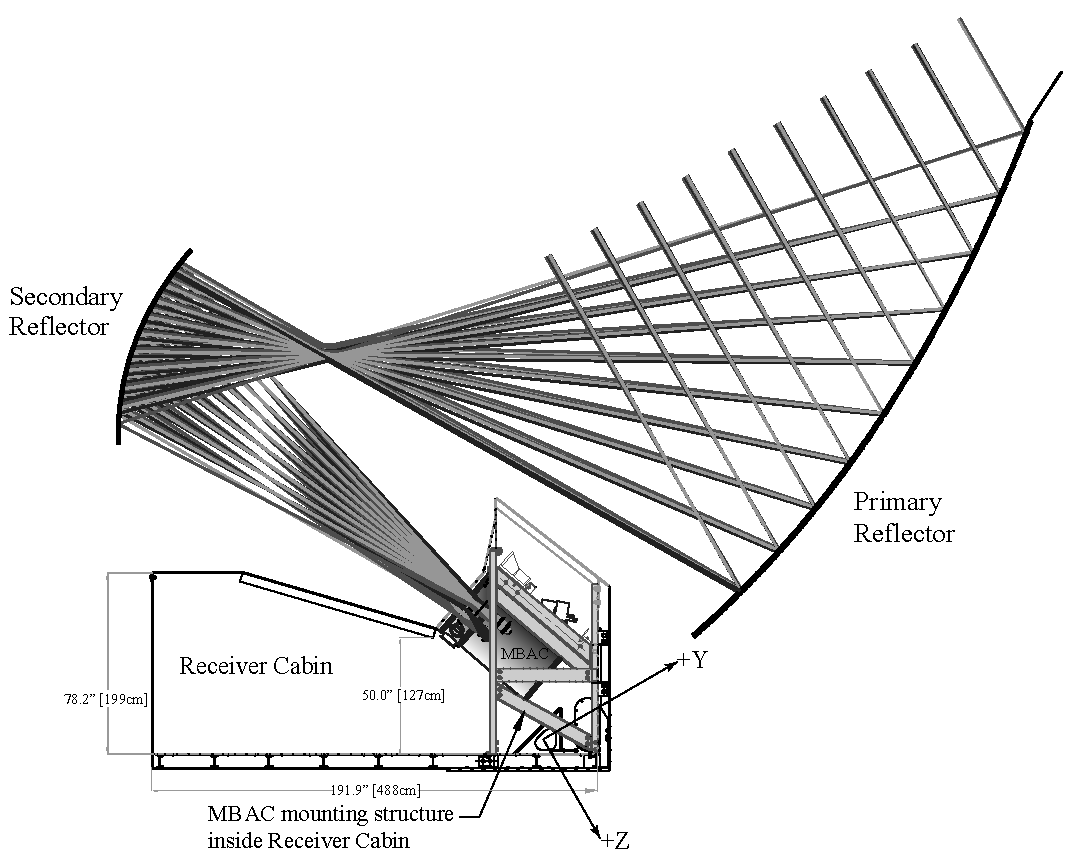
\includegraphics[width = \textwidth]{Figures/act_inst.pdf}
    \caption{Ray-trace diagram of the Atacama Cosmology Telescope~\cite{act_inst}.  The telescope is an off-axis Gregorian with two reflectors: the primary is 6\,m in diameter and the secondary 2\,m.  The rays trace into the Millimeter Bolometer Array Camera (MBAC) cryostat which houses the telescope's detectors.}
    \label{fig:act_inst}
\end{figure}

Since its inception in 2016, AdvACT has achieved many of its ambitious science goals~\cite{2016JLTP184772H}.  With improved sensitivity, ACTPol has measured the intrinsic temperature and polarization anisotropy at high-multipoles, which determines the spectral index of inflation, the primordial helium abundance, and neutrino properties~\cite{10.1117/12.857464}.  Galaxy clusters have also been studied from their Sunyaev-Zel’dovich effect, where CMB photons are scattered by high-energy electrons in the galaxy cluster along the line of sight~\cite{weinberg_cosmo}.  Soon to release its sixth data release (DR6), ACT has turned off observations and scientists will continue to use its groundbreaking data.

\begin{table}[b]
    \centering
    \begin{tabular}{|l|l|l|l|} \hline
        \textbf{ Parameter} & \textbf{MF}   &  \textbf{MF/HF}  & \textbf{HF}  \\ \hline \hline
        Number of Bolometers & 176 & 4430 &1006 \\\hline
        Angular Resolution (arcmin) & $7.1^{\prime}$/$4.8^{\prime}$ & $2.2^{\prime}$/$1.4^{\prime}$ & $0.9^{\prime}$ \\\hline
        Center Frequency (GHz) & 28/41 & 90/150 & 230\\\hline
    \end{tabular} \caption{ACT Key Characteristics~\cite{2016JLTP184772H}.}
    \label{tab:act}
\end{table}
\section{The Simons Observatory}
\begin{figure}[t]
    \centering
    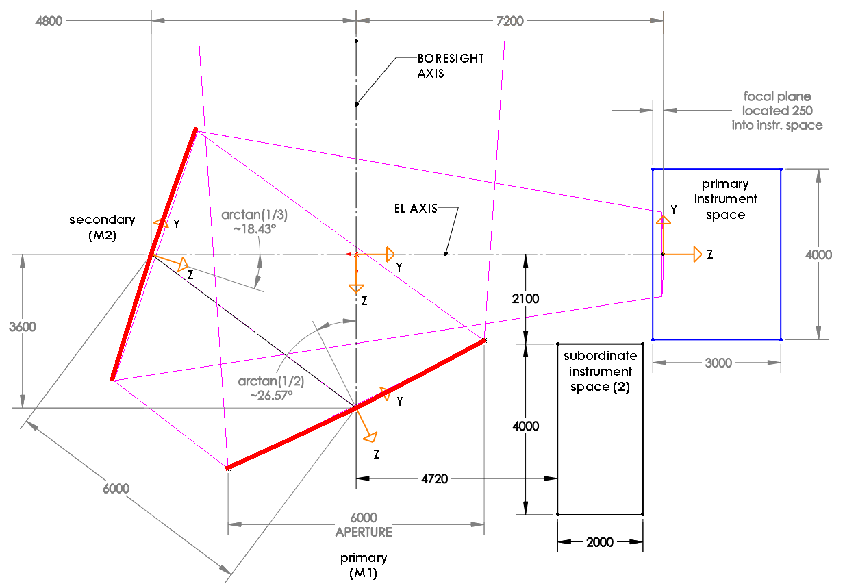
\includegraphics[width = .95\textwidth]{Figures/LAT_rt.pdf}
    \caption{Ray-trace diagram of the Simons Observatory Large Aperture Telescope~\cite{Parshley_2018}.  The telescope is a cross-Dragone with two reflectors, both 6\,m in diameter.  The rays trace into the Large Aperture Telescope Receiver (LATR) cryostat which houses 13 optics tubes.  The optics tubes guide the photons onto the detectors in the focal plane, which are cooled to 100\,mK.}
    \label{fig:so_inst}
\end{figure}
The Simons Observatory (SO) is a series of millimeter-wave telescopes designed to observe the Cosmic Microwave Background (CMB) temperature and polarization signals to an unprecedented sensitivity~\cite{gali18, so19}. With the combination of one Large Aperture Telescope (LAT)~\cite{xu/etal:2020c, zhu18, orlo18, coppi/etal:2018} and three Small Aperture Telescopes (SAT)~\cite{ali20}, the experiment will measure the temperature and polarization anisotropy of the cosmic microwave background with $\sim$\,70,000 background noise limited detectors operating at $\sim$\,100\,mK, covering six frequency bands centered on 27-280\,GHz (Table~\ref{tab:so}).

The resolution of SO will result in a catalog of extragalactic sources, including active galactic nuclei (AGN), dusty star-forming galaxies, and transient sources including Gamma Ray Burst (GRB) afterglows~\cite{so_science}.  SO expects to catalog 10,000-15,000 AGN sources at flux-densities above 7\,mJy~\cite{Tucci_2011}.  The low frequency coverage of SO will complement comparison work with other catalogs (e.g. VLA/VLASS, ASKAP/EMU, MeerKAT/MIGHTEE)~\cite{so_science}.  Dusty star-forming galaxies seen by SO will include local galaxies ($z<0.1)$ and high redshift galaxies (approximately $2<z<4$), and strong lensed galaxies beyond this range~\cite{Marrone_2017}.

\begin{table}[b]
    \centering
    \begin{tabular}{|l|l|l|l|} \hline
        \textbf{ Parameter} &  \textbf{LF} &  \textbf{MF}  &  \textbf{UHF}  \\ \hline \hline
        Number of Bolometers & $>$20,000& $>$20,000& $>$20,000\\\hline
        Angular Resolution (arcmin) & $3.3^{\prime}/3.0^{\prime}$ &$2.10^{\prime}/1.30^{\prime}$&$0.95^{\prime}/0.84^{\prime}$\\\hline
        Center Frequency (GHz) & 27/39 & 90/150 & 220/270\\\hline
    \end{tabular} \caption{SO Key Characteristics~\cite{Gudmundsson:21}.  The number of detectors are split evenly between the three frequency bands.  Note: the LF beam size is estimated by scaling down the MF and UHF beam sizes.}
    \label{tab:so}
\end{table}

\subsection{Large Aperture Telescope}

The Large Aperture Telescope (LAT) will map roughly 40\% of the sky at arcminute resolution~\cite{xu/etal:2020c}.   Figure~\ref{fig:so_inst} shows a cross-section and ray-trace of the LAT.  The primary mirror is 6\,m in diameter and constructed out of 77 individual adjustable panels, while the secondary mirror is 6\,m in diameter and constructed out of 69 adjustable panels \cite{gali18}.

Light from the sky is then reflected into the LAT Receiver (LATR), which houses up to thirteen optics tubes~\cite{Xu_2021}.  The LATR optics tubes re-image the optics onto the detector arrays (three detector arrays per optics tube).  Chapter~\ref{ch:ot_holo} presents radio holography measurements of the LAT optics tube, where I characterize the optical performance of the LAT Receiver optics tube.

\begin{figure*}[ht]
    \centering
    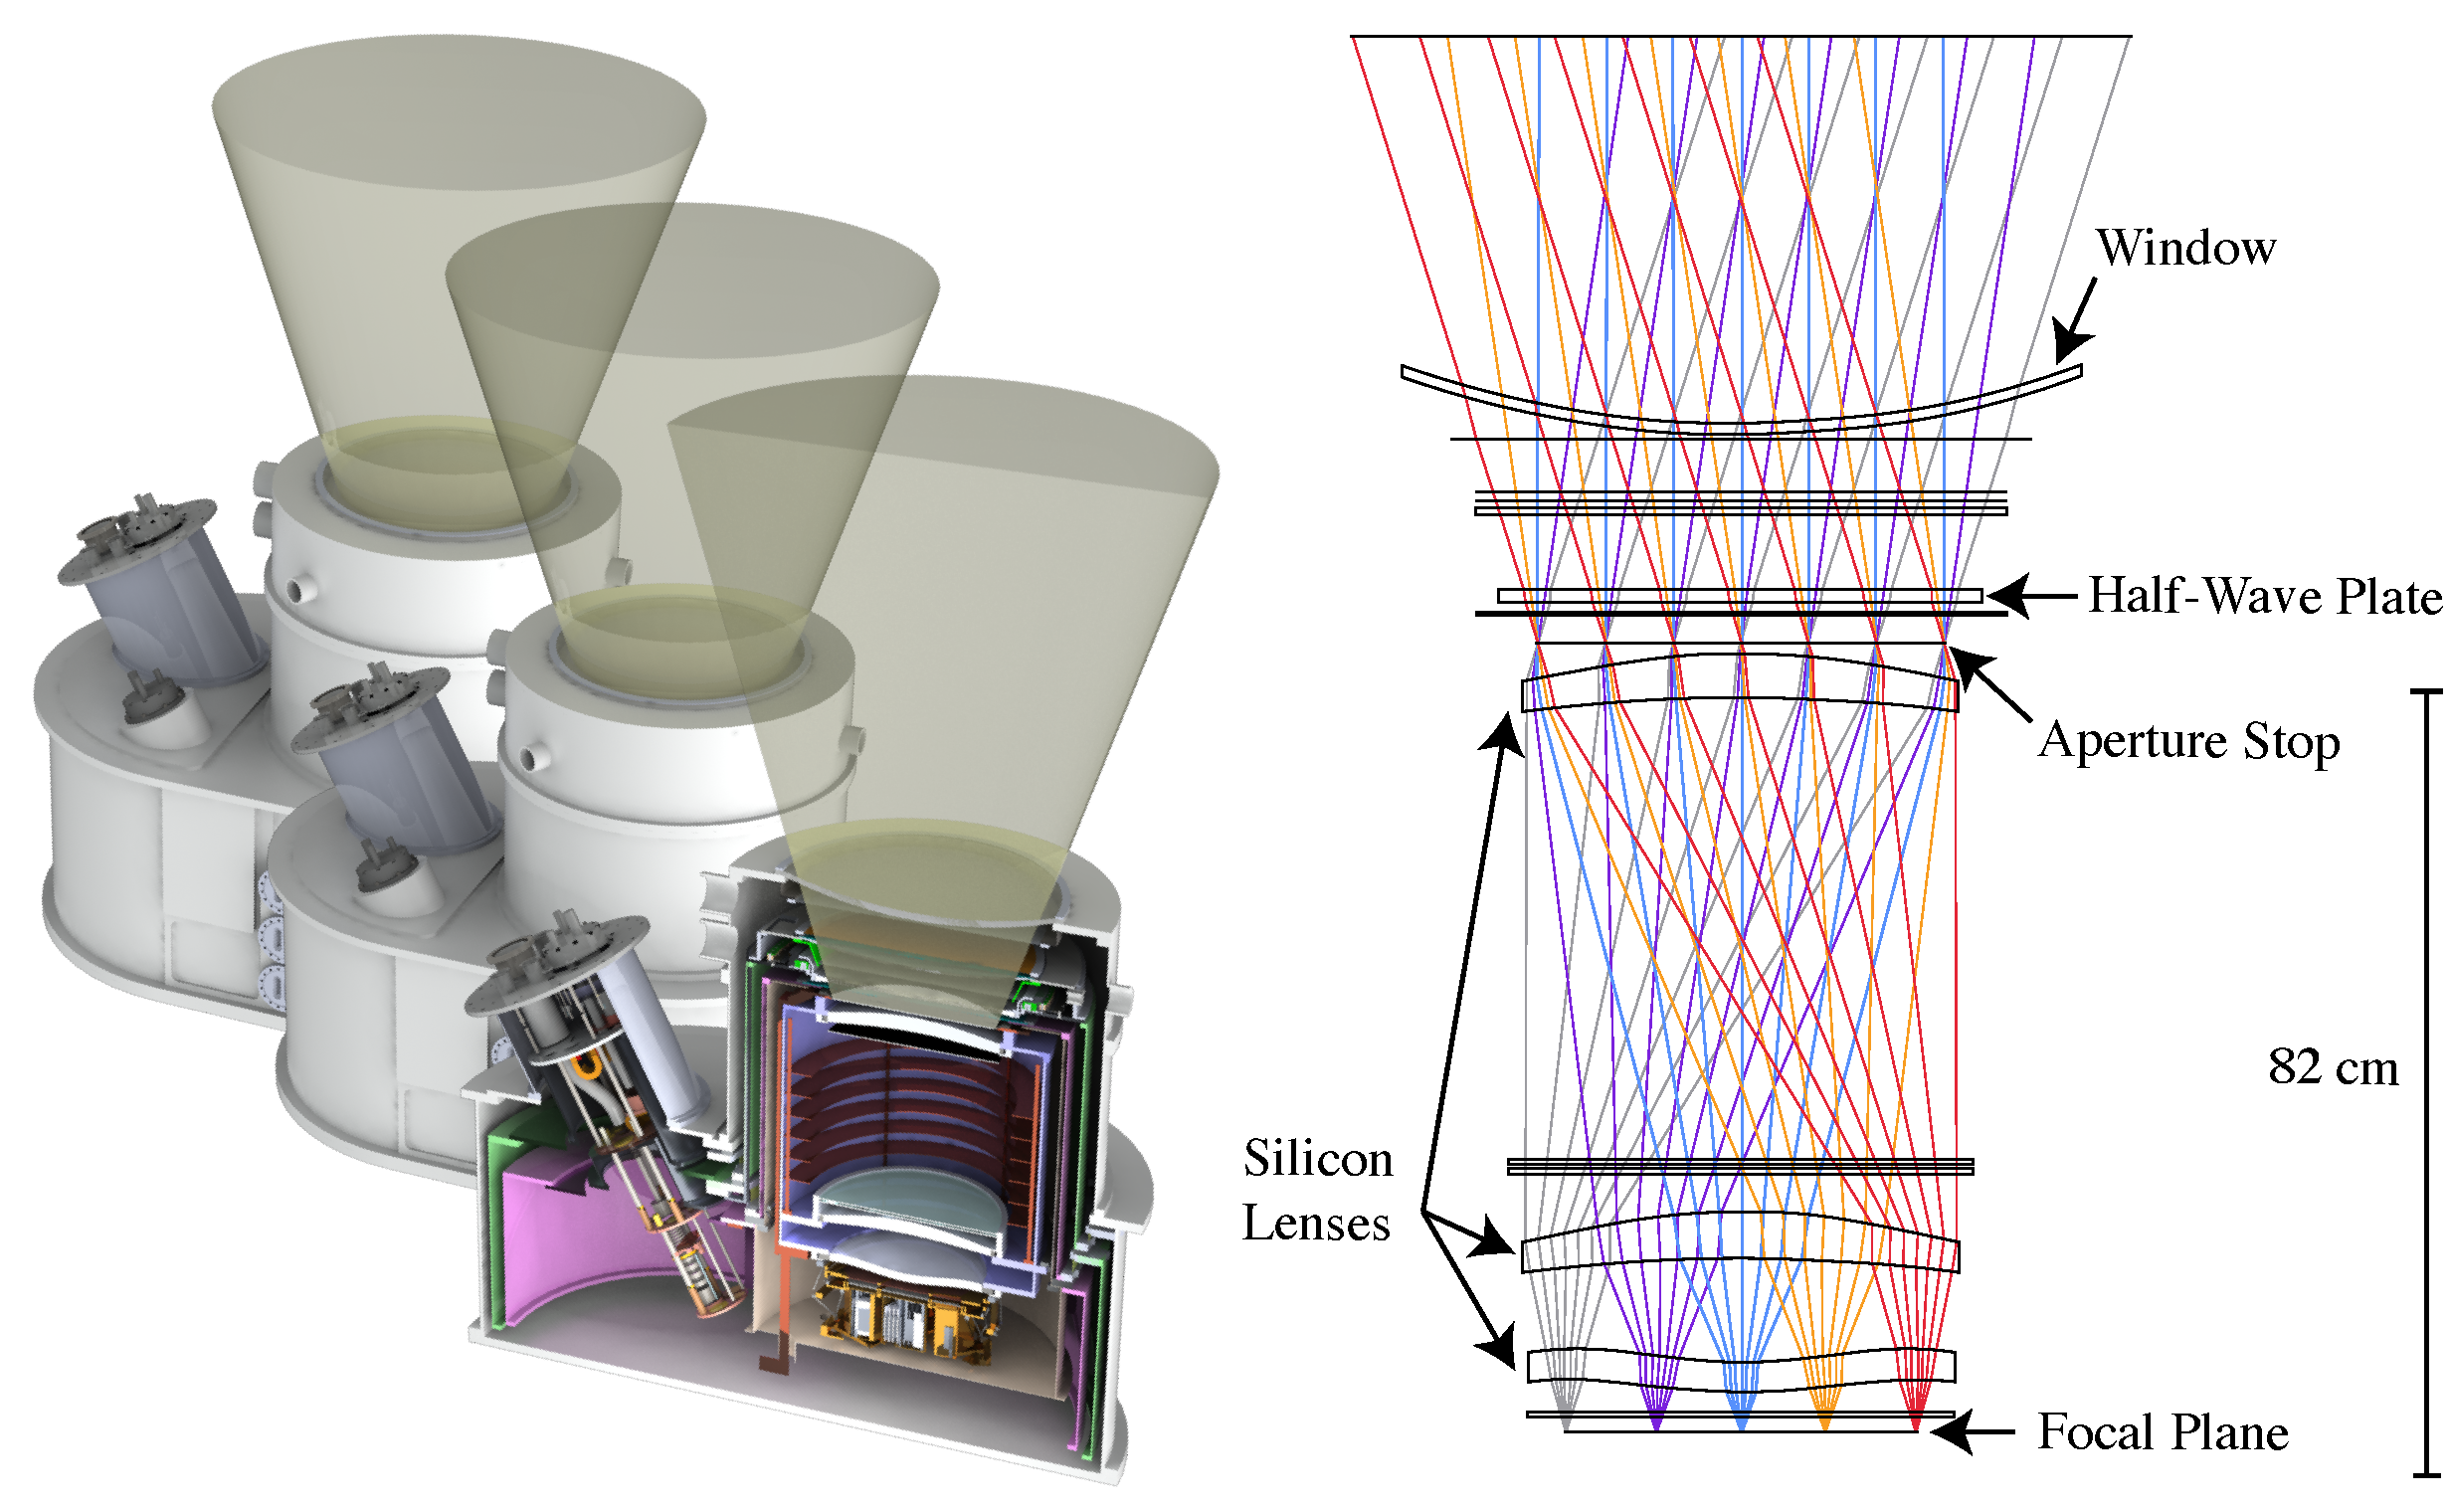
\includegraphics[width = \textwidth]{Figures/SAT3.pdf}
    \caption{Left: Three Small Aperture Telescope cryostats, with the front cross-section showing the inner optics tube.  Right: Ray-trace diagram of the Simons Observatory Small Aperture Telescope~\cite{2020SPIE11445E7LK}.}
    \label{fig:sat3s}
\end{figure*}

\subsection{Small Aperture Telescope}

The Small Aperture Telescope (SAT) optical design is a 0.42\,m diameter refractive telescope (Figure~\ref{fig:sat3s}).  Three SATs will measure the largest angular scales visible from the Atacama Desert.  In total, the three SAT's will hold roughly 30,000 cryogenic detectors, where the SAT is targeting to characterize the CMB on degree angular scales.  In Chapter~\ref{ch:sat_holo}, I present radio holography measurements of the SAT optics tube.

The SAT is a purely refractive telescope.  Figure~\ref{fig:sat3s} shows the ray-trace from the focal plane out the SAT window.  Light enters through a 3\,mm thick ultra-high molecular weight polyethylene hexagonal window with an anti-reflection coating~\cite{zhu18}.  A Cryogenic Half-Wave Plate (CHWP) polarization modulator then reconstructs the polarization of the CMB at 40\,K.  A 1\,K Lyot stop is the first cold optical element, and is followed by the SAT refractor.  Three anti-reflection coated silicon lenses~\cite{Datta:13,golec20} re-image the light onto seven hexagonal detector arrays.   Photons are then coupled onto the detectors by individual feedhorns.  The focal plane of each optics tube houses seven hexagonal detector arrays and are cooled to 100\,mK.

\subsection{The Status of the Simons Observatory}

The Simons Observatory is currently being deployed in the Parque Astronomico located in the Atacama Desert in Chile (Figure~\ref{fig:act_so_site}). The telescope site is situated at an elevation of 5,200 meters near the peak of Cerro Toco at $22 ^\circ$ 57' S, $67^\circ$47' W.  The arid conditions and elevation at the site minimize contamination to millimeter wave signals from water vapor.

Integration and testing occurs in parallel with deployment, as the rollout of the Simons Observatory continues.  In the year to come, SO will begin observations and characterize the CMB with unprecedented sensitivity, with many discoveries of the nature of our universe to come.
\chapter{Metamaterial Microwave Absorber (MMA) and its Cryogenic Applications}

\section{Introduction}
\section{Optical Design}
\section{Optical Testing}
\subsection{Optical Hardware}
\subsection{Receiver Electronics}
\subsection{Measurement}
\section{Reflection Measurement}
\section{Scattering Measurement}
\section{Future Applications}
\section{Conclusion}
\chapter{Reflectometry Measurements of the Loss Tangent in Silicon at Millimeter Wavelengths}
\section{Introduction}
\section{Procedure}
\subsection{Optical Hardware}
\subsection{Receiver Electronics}
\subsection{Samples: Neutron-irradiated and Intrinsic Silicon}
\section{Reflectometry and Transmissivity}
\subsection{Modeling}
\section{Results}

\chapter{The Simons Observatory: Characterizing the Large Aperture Telescope Receiver with Radio Holography}
\label{ch:ot_holo}
\section{Introduction}
\section{The SO Large Aperture Telescope Optics Tubes}
\section{Measurement Approach}
\subsection{Cryogenic Receiver}
\subsection{Holography System}
\section{Results and Interpretation}
\subsection{Propagation of Fields}
\subsubsection{Fields at Secondary Illumination}
\subsubsection{Far-Fields}
\section{Filter Removal}
\section{Public Code}
\subsection{Optics Simulation}
\subsection{Open Source Holography}
\section{Conclusion}
\chapter{The Simons Observatory: Characterizing the Small Aperture Telescope with Radio Holography}
\label{ch:sat_holo}
This chapter presents holography measurements of the Simons Observatory Small Aperture Telescope at the University of California, San Diego, and preliminary characterization of its optical performance.
\section{Introduction}
The Simons Observatory (SO) will employ three Small Aperture Telescopes (SATs) to measure the largest angular scales visible from the Atacama Desert in Chile.  One SAT has an aperture diameter of 0.42\,m and will measure roughly 10\% with more than 300,000 bolometer detectors across the three SATs~\cite{2020SPIE11445E..7LK}.  Each SAT contains two frequency bands; Mid-Frequency bands are centered at 93 and 145\,GHz, Ultra-High-Frequency bands are centered at 225 and 280\,GHz, and Low-Frequency bands are centered at 27 and 39\,GHz.  

We present the laboratory testing of the MF Small Aperture Telescope using the technique of near-field radio holography.  "Holography" refers to the measurement of the complex monochromatic electric field wavefront using the interference between a modulated and reference signal.  Radio holography takes advantage of the antenna theory relationship: the far-field radiation pattern of a reflector antenna is the Fourier Transformation of the field distribution in the aperture plane of the antenna~\cite{alma_holog}.

\begin{figure*}[t!]
    \centering
    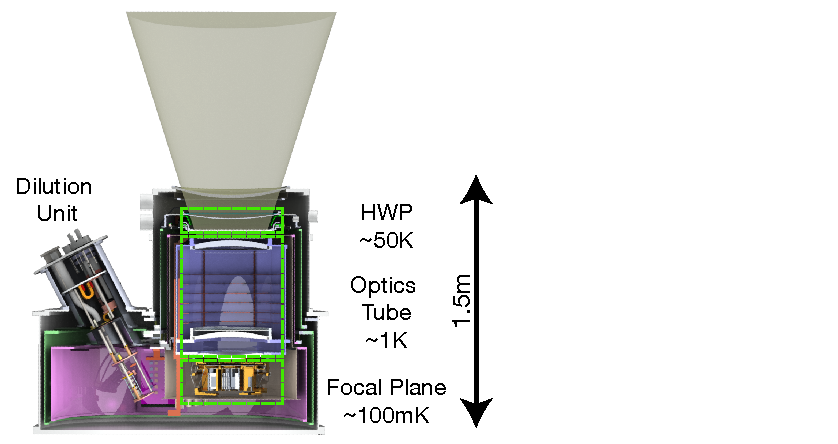
\includegraphics[width = .95\textwidth]{Figures/sat_optics.pdf}
    \caption{Left: Cross-section of the Small Aperture Telescope (SAT) optics tube.  Right: SAT cryostat used in holography testing.}
    \label{fig:sat_optics}
\end{figure*}

Near-field holography of the SAT maps the wavefront emerging from the cryostat.  Using Fresnel diffraction (FD)~\cite{Goodman2005-ne}, these measured fields can be propagated to determine the far-field beam pattern of the telescope fed by this feedhorn receiver.  Moreover, these beams are useful for the identification and mitigation of optical problems within the receiver (i.e. optical aberrations, focus, scattered power, etc.).  These measurements enable a detailed verification of system-level optical performance prior to the deployment of a receiver on a telescope.

In Section~\ref{sec:sat_optics_tube} we describe the optical design and components of the SO SAT optics tube.  In Section~\ref{sec:satot_meas_method} we describe the measurement approach including the cryogenic receiver (\ref{sec:sat_cryo_rec}) and holography hardware (\ref{sec:sat_meas_hardware}) required for measuring beam maps (full details can be found in Appendix~\ref{sec:appendix_hardware}).  In Section~\ref{sec:sat_results} we present the measured beam maps.   Section~\ref{sec:sat_prop_fields} discusses analysis methods to propagate the measured beams into the far-field using FD.  We conclude with a discussion of future applications of this approach in Section~\ref{sec:sat_discussion}.  
\section{SO Small Aperture Telescope Optics Tubes Design}
\label{sec:sat_optics_tube}

\begin{figure}[t!]
    \centering
    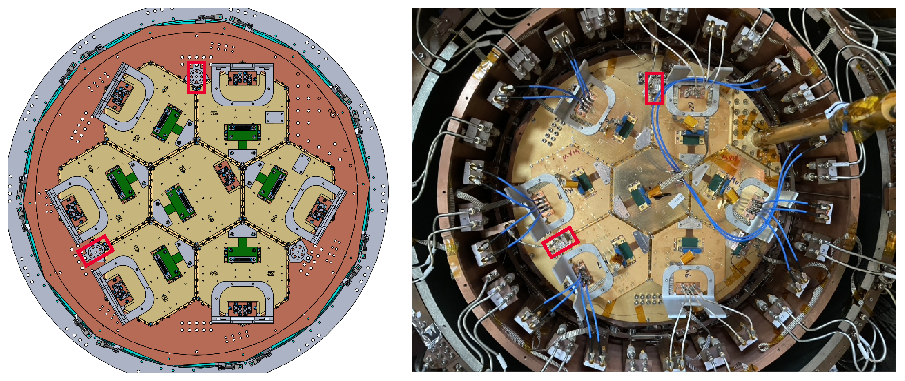
\includegraphics[width = \textwidth]{Figures/sat_fpa.pdf}
    \caption{SAT Focal Plane.  The two holography receivers are outlined in red, separated by $120^{\circ}$.  Two receivers are installed for redundancy, but also served as a useful tool when characterizing systematics (such as "ghosting", or spurious signal in the beam maps, and polarization effects).}
    \label{fig:sat_fpa}
\end{figure}

Here we provide an overview of the SAT optics, starting at the window of the telescope and ending at the detectors.

\begin{figure}[t!]
    \centering
    \includegraphics[width = \textwidth]{Figures/sat_exp.png}
    \caption{Lab photos of the holography setup on the SAT.  Left: The holography source, covered in a sheet of eccosorb to control scattering, is centered above the SAT window and points directly into the SAT.  Right:  The holography electronics sit on a cart next to the SAT readout.}
    \label{fig:sat_hardware}
\end{figure}

Light enters through a 3\,mm thick ultra-high molecular weight polyethylene hexagonal window with an anti-reflection coating~\cite{zhu18}.  A Cryogenic Half-Wave Plate (CHWP) polarization modulator then reconstructs the polarization of the CMB at 40\,K.  For the duration of these holography measurements, the CHWP is held at a fixed angular orientation.  A 1\,K Lyot stop is the first cold optical element, and is followed by the SAT refractor.

The SAT optics is purely refractive; three anti-reflection coated silicon lenses~\cite{Datta:13,golec20} control the beam size and shape onto seven hexagonal detector arrays.  The SAT lenses are the largest Si lenses used for a CMB telescope to date~\cite{ali20}.  Baffles line in the inside of the SAT refractor to control spurious scattering.  Photons are then coupled onto the detectors by individual feedhorns. Seven hexagonal detector arrays are housed in the focal plane of the optics tube at 100\,mK.

\section{Measurement Approach}
\label{sec:satot_meas_method}
Here, we describe the hardware in two sections: 1) a cryogenic optics tube and 2) the holography system comprised of a source, correlation receiver, and motion system.
\subsection{Cryogenic System}
\label{sec:sat_cryo_rec}
The optics tube is housed in the SAT cryostat\cite{2020SPIE11445E..7LK}.  The cryostat holds and cools the optics tube and provides support for detector readout.  This setup supports up to seven detector arrays (Fig.~\ref{fig:sat_fpa}).   In the test configuration, all bolometric arrays~\cite{2022arXiv220104507H} are filled in the focal plane, and two holography feedhorns are added to the edges of the focal plane, each separated by $120^{\circ}$.



The holography detectors consist of a feedhorn  identical to that used for the bolometric detectors, but with standard wave guide flanges at the outputs. A receiver consisting of a round to rectangular wave guide transition and a harmonic mixer is attached to this feed array.  The mixer was designed to operate from 70-110\,GHz, but was found to operate satisfactorily up to 170\,GHz. For operational simplicity, we used this mixer over our full frequency range from 80-170\,GHz.

Two identical receivers are installed in the focal plane for redundancy.  Two 0-18\,GHz coaxial connections were made from the receiver to connectors at the cryostat wall.  These coaxes are heat sunk at various stages between the focal plane, which was operated at 4\,K while doing holography, and the 300\,K cryostat wall.  A separate cool down was used to measure the loss along these coaxial feed lines.  The loss  was found to be 23\,dB at the LO frequency (10-13\,GHz).  Accurate knowledge of the loss along the feed lines is critical for providing the correct amount of power to the mixers in the focal plane.  The loss at the interference frequencies (IF) (100\,MHz) is significantly lower and not critical to the function of this system.

\subsection{Holography System}
\label{sec:sat_meas_hardware}

Figure~\ref{fig:setup} shows a schematic overview of the holography hardware.  Two millimeter-wave sources are used to measure the full SO MF band: F90 (80-120\,GHz) and F150 (130-170\,GHz).  Only one is mounted at a given time.  These sources are broadcast into the receiver using standard gain feed horns held close to the window ($\approx10$\,cm).

A motorized two-dimensional stage holds the source and is mounted on a support structure above the SAT.  During a measurement, the source (frequency is fixed) is moved over a $80\times80$\,cm range with 1\,cm steps.  One map takes roughly 2 hours to complete.

A common local oscillator (LO2 in Figure~\ref{fig:setup}) is fed to two harmonic mixers: 1) picked off from the source and 2) at the output of the cryogenic receiver.  The IF signal from both mixers in the 0-100\,MHz band is amplified and passed to a digital correlator (Casper ROACH2 ~\cite{roach2}) which computes the complex correlation between the two signals~\cite{ches18}.  The FPGA on the ROACH2 board outputs the amplitude and the phase of the correlated output, subdivided into a number of 100\,kHz wide bins.  Only the bin associated with the IF frequency is used in subsequent analysis.  The software to program and analyze output from the FPGA is made public on the \textit{McMahonCosmologyGroup} GitHub page in a package called \verb|holog-exp|~\cite{holog-exp}.  Appendix~\ref{app:holog} provides further details to the hardware of the holography setup.

Due to the presence of the HWP, the source's signal is polarized upon entering the optics tube.  Therefore, at each frequency, we measure two beam maps: with a waveguide twist, and without a waveguide twist.  This allows us to measure the response of the optics tube at two source polarizations (the waveguide twist changes the source polarization by $90^{\circ}$).

 \begin{figure}[t!]
    \centering
    \includegraphics[width = .47\textwidth]{Figures/sat_radbin.png}
    \includegraphics[width = .47\textwidth]{Figures/sat_fwhm.png}
    \caption{Left: Preliminary near-field beam shape of the SAT in MF-1.  Beams are averaged over all frequencies measured, and the averaged beam is then radially averaged to get the near-field beam profile.  Right: Preliminary beam sizes of the SO SAT in MF-1.  Far-field beams measured with holography (blue) are radially binned and the FWHM is obtained from the resulting 1D beam profile.  Simulations are obtained using a diffractive optics simulation, and plotted are where the measured beam sizes are within 5 and 10\%.}
    \label{fig:sat_fwhm}
\end{figure}

\section{Results and Interpretation}
\label{sec:sat_results}

\subsection{Near-Field Beam Maps}
Figure~\ref{fig:sat_beams} and ~\ref{fig:sat_phases} show the measured power and phase of the beam maps, respectively, at each frequency.   A variable attenuator at the output of the source was used to optimize the amount of signal entering the optics tube, to ensure power was not too high such that the measurement was saturated, but to also ensure the signal was high enough for signal-to-noise greater than 35\,dB.

Each beam map is labeled either $0^{\circ}$ WG, with a straight waveguide at the source output, or $90^{\circ}$ WG, with a waveguide twist at the source output.  These labels also correspond to the $E_x$ and $E_y$ fields.  We assume the source and receiver to be misaligned; to account for this, we rotate the two beams by $\theta$ which is fit to minimize $E_y^{'}$:

\begin{equation}
\begin{bmatrix}
 E_x^{'} \\
 E_y^{'}
 \end{bmatrix} = 
\begin{bmatrix}
 \cos(\theta) & \sin(\theta) \\
 -\sin(\theta) & \cos(\theta)
 \end{bmatrix}
\begin{bmatrix}
 E_x \\
 E_y
 \end{bmatrix}
 \end{equation}
 
The shape of the main beam was found to be in good agreement with simulations at all frequencies (Figure~\ref{fig:sat_fwhm}).  The phase measurement indicates the direction of the beam as it exits the window.  Figure~\ref{fig:sat_phases} shows the phases across all frequencies; the unwrapped phase is a gradient due to the beam exiting the window at an angle (as the holography detector is far-off from bore sight in the focal plane).  However, we further note the change in phase gradient as a function of frequency and have modeled this to be an aliasing effect of the measurement.

 \begin{figure*}[t!]
    \centering
    \includegraphics[width = .75\textwidth]{Figures/farfield_sat.pdf}
    \caption{Preliminary far-fields of the SAT optics tube in the MF-1.}
    \label{fig:farfields_sat}
\end{figure*}

\subsection{Propagation of Fields}
\label{sec:sat_prop_fields}

The performance of the SAT optical system is assessed in detail by using the amplitude and phase of the measured beams to calculate the far-field.  This is carried out by using the Fourier relationship between the near-field $E(x,y)$ and far-field $B(\theta_x,\theta_y)$ beams \cite{McIntosh2016,alma_holog}:
\begin{equation}
    B(\theta_x,\theta_y) = \int_{\text{aperture}} E(x,y) e^{ i \frac{2\pi}{\lambda} (\theta_x x + \theta_y y )} dx \, dy 
\end{equation}
where the complex electric field $E(x,y)$ is integrated over the area of the aperture, $\theta_x$ and $\theta_y$ are the on-sky angular coordinates, and $\lambda$ is the wavelength.  The resulting (preliminary) far-fields are shown in Figure~\ref{fig:farfields_sat}.  The measured beam sizes are consistent with the predicted F90 FWHM of XXX arcmin.

\section{Conclusion}
\label{sec:sat_discussion}

We have presented holography measurements of the SO SAT optics tube and analysis methods determining its optical performance.  We further provide an open-source package for simulating near-field holography measurements and propagating the measurements into the far-field using Fourier optics.  From these data, we characterize the optical performance of the LATR optics tube.  We compare near- and far-field measurements to simulations.  After propagating the beams to the far-field, we find the SAT beam FWHM to be (XXX) in the F90 band.

We also provide \verb|sosat-optics|, an open-source software package, which models the SAT holography measurements and is customizable to include arbitrary optics and adaptable for other optics experiments~\cite{sat_sim_model}.  The approach demonstrated here follows the successful characterization of the Large Aperture Telescope Receiver tester, and is broadly applicable to other millimeter-wave optical systems~\cite{chesmore2022}.  The ability to characterize the optical performance and systematics of the optics tube allowed us to determine the SAT optics is in focus and that the beam is within requirement for SO science. 

\begin{figure}
    \centering
    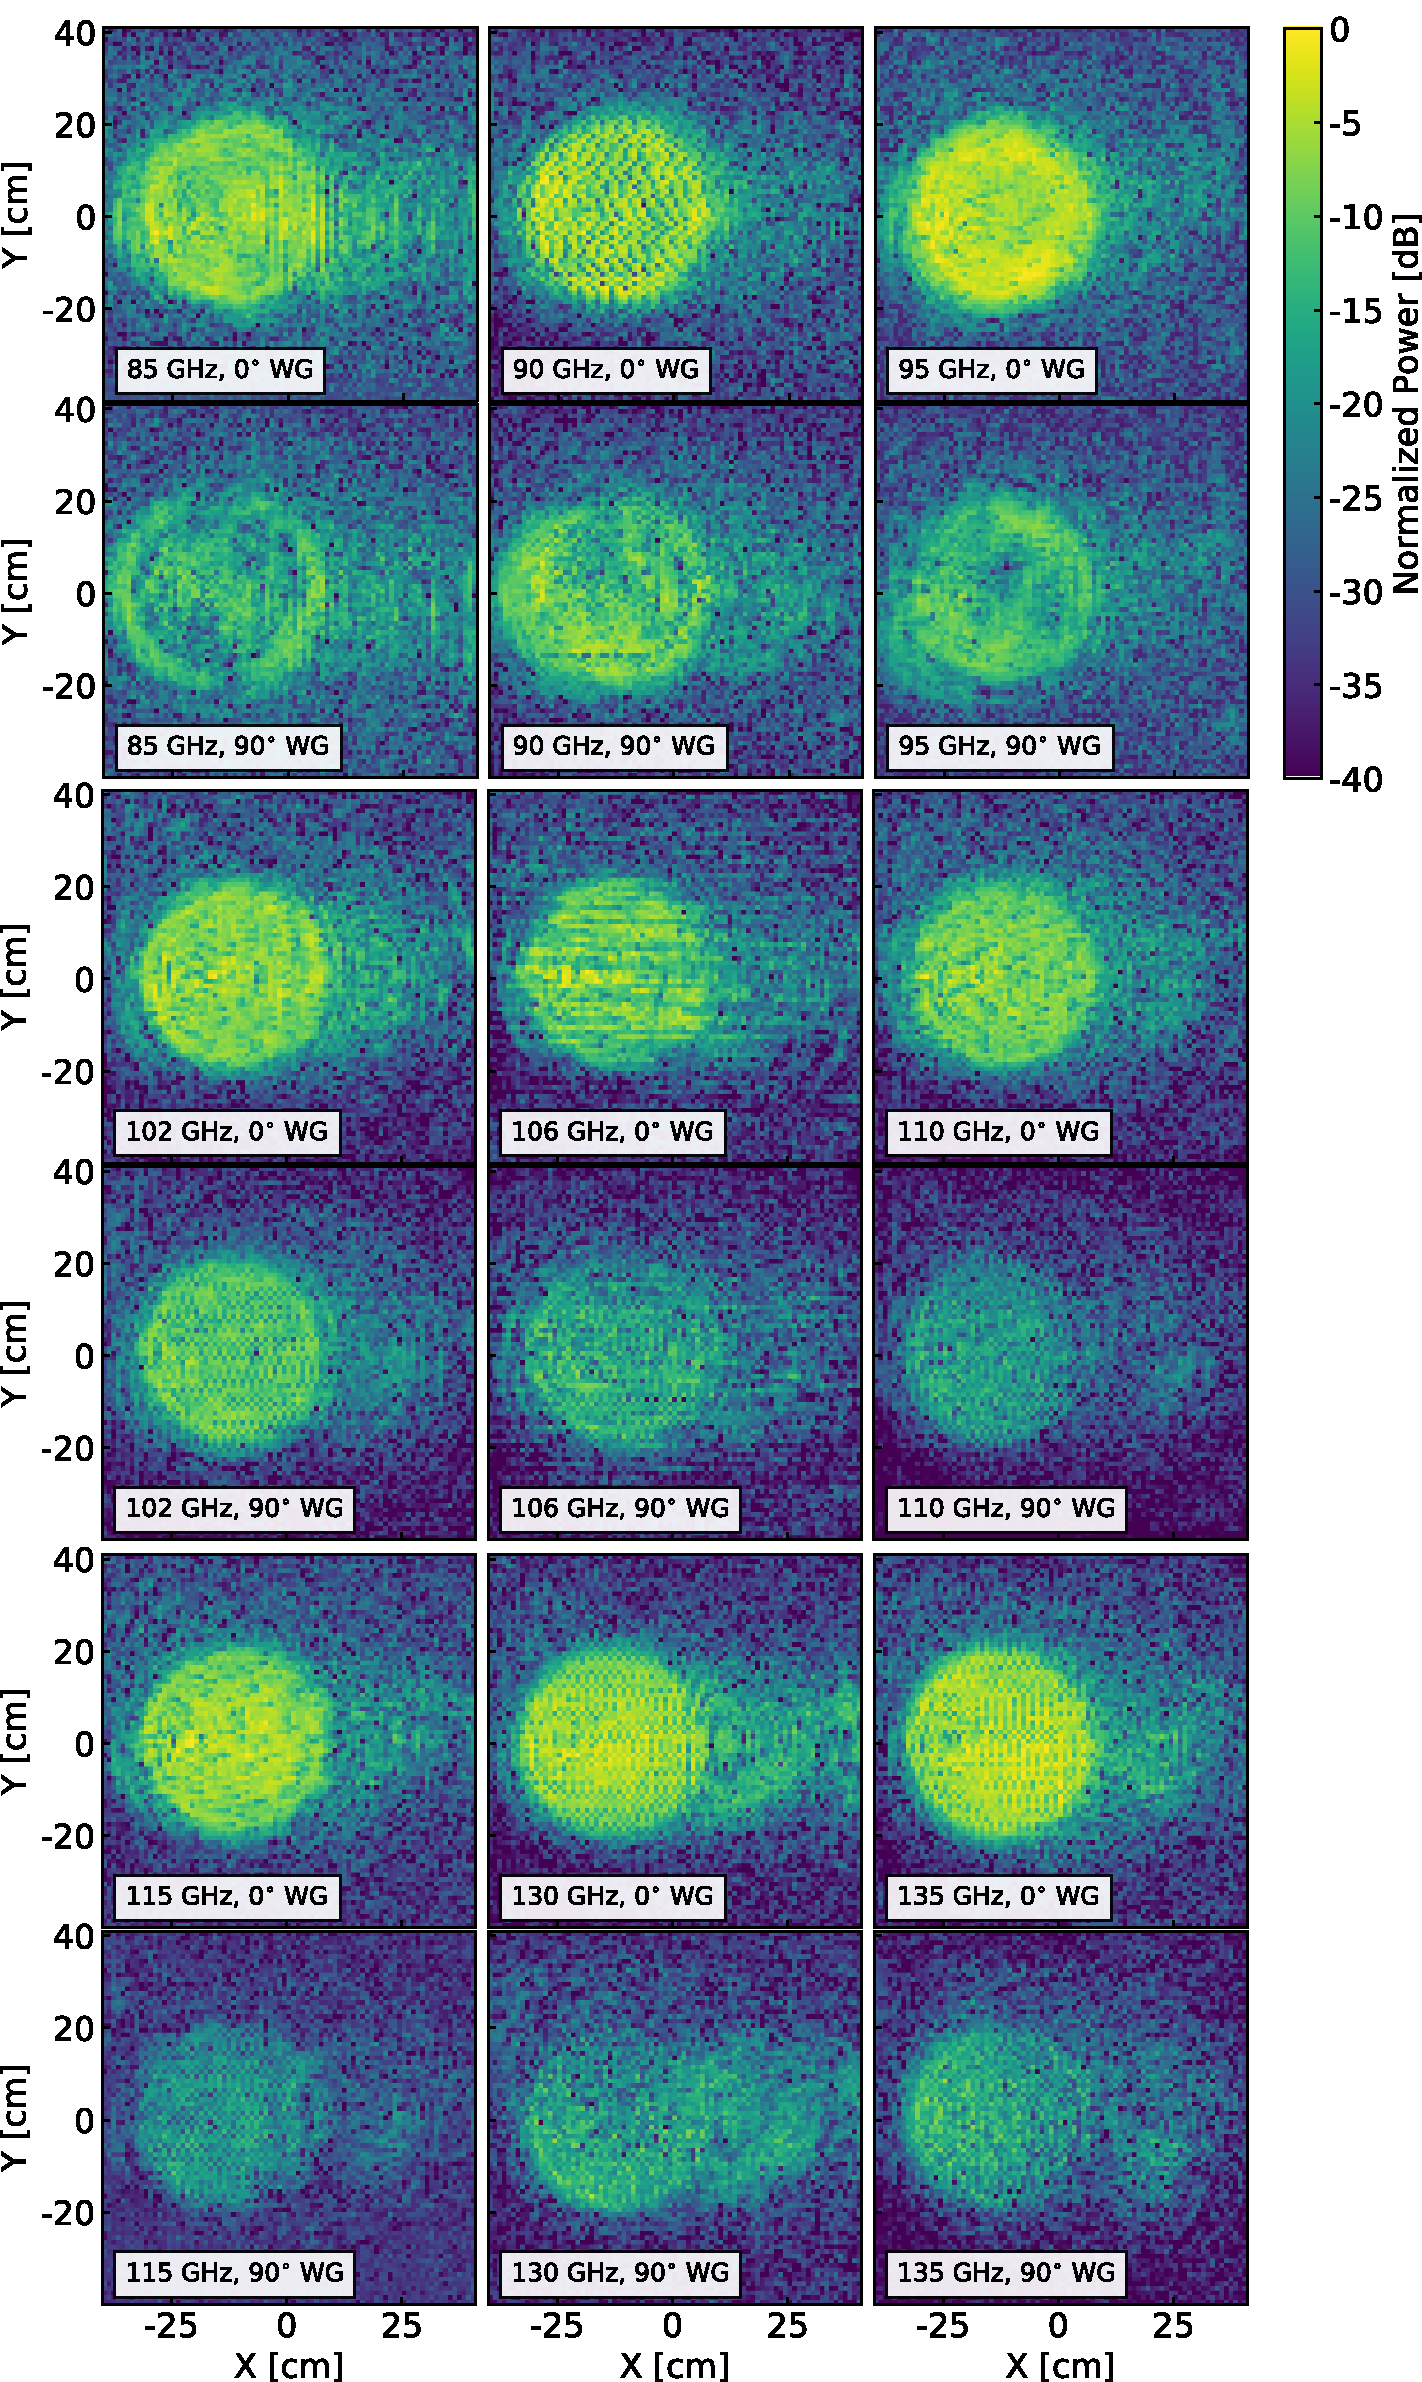
\includegraphics[width=.75\textwidth]{Figures/sat_beams.pdf}
    \caption{Normalized power of Small Aperture Telescope beams.}
    \label{fig:sat_beams}
\end{figure}

\begin{figure}
    \centering
    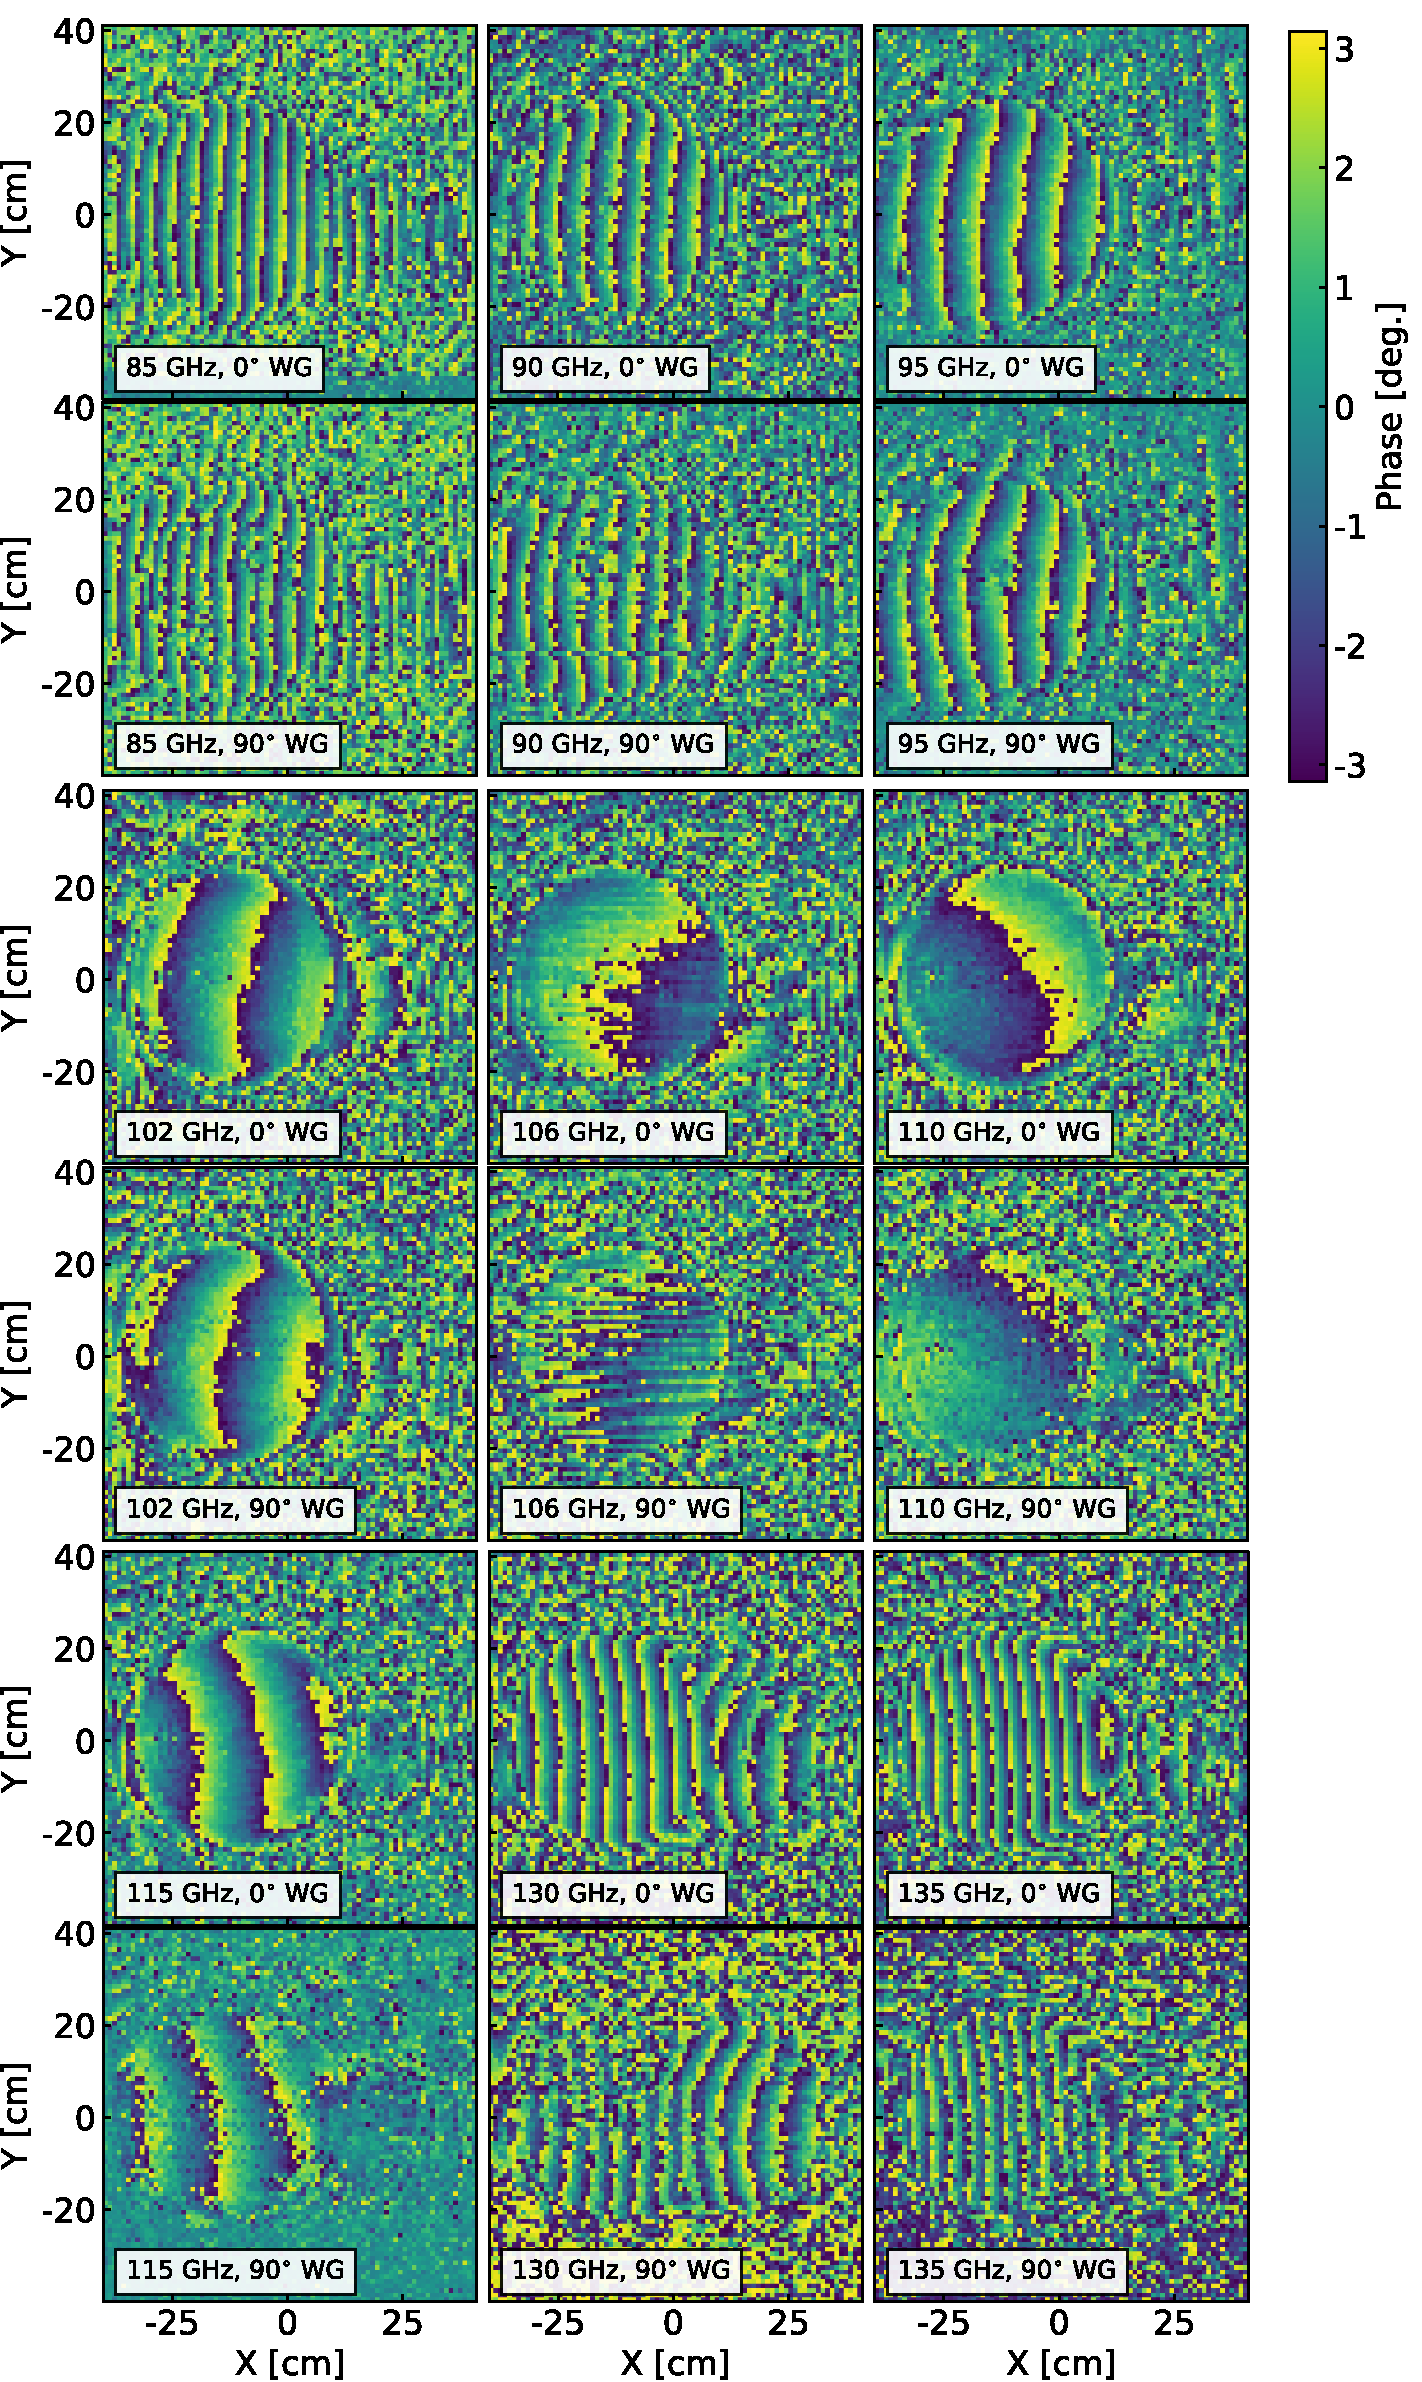
\includegraphics[width=.75\textwidth]{Figures/sat_phase.pdf}
    \caption{Phase (wrapped) of Small Aperture Telescope beams.}
    \label{fig:sat_phases}
\end{figure}

\chapter{The Simons Observatory Large Aperture Telescope}

\section{Introduction to Large Aperture Telescope}
\section{HoloSim-ML: machine learning applied to the efficient analysis of radio holography measurements of complex optical systems}
\subsection{Introduction}
\subsection{Motivation}
\subsection{Beam Simulation}
\subsection{Holography Analysis}
\subsection{Panel Fitting with Machine Learning}
\subsection{Measurement Practicalities and Robustness of Method}
\subsection{Public Code}
\subsection{Conclusion}
\chapter{The Atacama Cosmology Telescope: point source analysis of beams for DR6}
\label{ch:actbeams}

\section{\label{sec:act_intro}Introduction}
\setcounter{footnote}{0}

The Atacama Cosmology Telescope (ACT) is a 6\,m off-axis Gregorian telescope located at an altitude of 5190\,m in the Atacama Desert of northern Chile. It is designed for millimeter wavelength observations of the cosmic microwave background (CMB) at arcminute resolution.  The telescope and receiver are described in \cite{fowler_2007} and \cite{thornton_2016} respectively. 

This paper describes an alternative method for determining the optical response of the telescope based on stacking point source observations.  This data release includes temperature and polarization data collected by ACT between 2017 and 2021, covering roughly 18,000 square degrees of the sky~\cite{thornton_2016}.

Determining the optical response, or "beam", quantifies how the instrumental response is suppressed at small angular scales as a result of the finite resolving power of the optics.  For this reason, understanding the telescope beam and its uncertainty is critical for achieving the science goals of ACT.  Because the beam has to be de-convolved from the sky maps in order to perform cosmological analysis, incorrectly characterizing the beam directly biases any science by mimicking a spurious scale-dependent signal.  Therefor, in order to achieve the science goals set out by ACT, characterization of the instrument beam is crucial.  Besides the beam of the instrument, it is also important for a polarimetric instrument like ACT to quantify the amount of temperature-to-polarization leakage. We describe this type of leakage in terms of a so-called "leakage beam", quantifies the amount of leaked signal from Stokes I to Stokes Q or U at a given angular scale.

Previous work to characterize the ACT instrument beam have done so with planet maps (~\cite{hasselfield_atacama_2013,louis_2017,naess_2014}).  Planets served as the best candidates for beam characterization of the telescope~\cite{Lungu_2022}.  Specifically, observations of Uranus achieve adequate signal-to-noise without exceeding the dynamic range of the instrument.  Here, we present a novel technique to characterize the instrument beam with map data, which we refer to as "stacking" of the point-sources in a map's catalog.  This work provides a detailed recipe for characterizing an instrument's beam using full map data, which we apply to the ACT DR6 maps.  This method provides a validation of the Uranus-derived beam both in temperature $T$ and in the $T\rightarrow E$ and $T\rightarrow B$ leakage.  Such a novel validation is necessary because the Uranus observations are separate observations made with a different strategy than the full maps, have different noise properties and were made using a different map-making technique.  The point-source stacking method, presented here, uses the same observations which we use for cosmology, thus providing a check to the beam and leakage inferred from Uranus observations.

\begin{figure*}[t]
\vspace{1em}
    \centering
    \includegraphics[width=\linewidth]{Figures/pt_src_dist.png}
    \caption{Distribution of the total number of point sources that were in the catalog (faded colors) and ultimately became part of the final beam analysis (solid colors) for all arrays combined, shown by observing seasons from 2017--19.
    }
    \label{fig:ptsrc_select}
    \vspace{1em}
\end{figure*}

The paper is organized as follows. 
In \S\ref{sec:obs} we describe the observations and catalog used to stack point sources and characterize the ACT beams.  In \S\ref{sec:stack} we explain the stacking process, starting from an input map and producing a stacked beam profile.  In \S\ref{sec:sim_pipe} we describe the steps of the map simulation pipeline, then going from simulated point-source maps to a model of the ACT beams and their covariance.  In \S\ref{sec:act_results} we present the results from the stacking method, including the stacked temperature to polarization leakage, and the temperature beam radial profiles.  Finally, in \S\ref{sec:act_disc} we discuss assumptions made in the analysis and future directions for ACT beam characterization.

\begin{figure*}[t]
    \centering
    \includegraphics[width = \textwidth]{Figures/ptsrc_map.png}
    \caption{Spatial distribution of point sources from catalog(grey) and used in stacking(colored).  The colorbar shows the flux of the special(ML) sources, which are plotted as triangles(circles).}
    \label{fig:ptsrc_map}
\end{figure*}

\section{Observations}
\label{sec:observations}

The DR6 data were obtained using three dichroic detector arrays, PA4, operating at 150 and 220\,GHz, PA5, operating at 98 and 150\,GHz, and PA6, operating at 150 and 220\,GHz.

\textcolor{red}{Adri:}
\label{sec:obs}
\begin{itemize}
    \item description of CMB maps
    \item from 2017-2021 in these f bands and this patch of the sky
    \item ML vs. Special point source description
\end{itemize}

\section{Methods}
\label{sec:stack}
Here we walk through the stacking process from input map to beam profile.  
\subsection{Point-source Selection}
\label{subsec:ptsrc_sel}
Prior to stacking, we characterize each point source to determine whether they are suitable for stacking.  The number of point sources used for the point source analysis versus the total number of point sources in the catalog is shown in Figure~\ref{fig:ptsrc_select}.

\subsubsection{Select on Catalog}
\label{subsubsec:cat_sel}
For ease of interpretation, a sky mask is applied that is similar to those used by the various cosmological analysis. This mask removes regions with strong Galactic emission (based on the 353 GHz Planck data) and significantly noisy regions on the sky.  The point source catalog has been estimated from the DR6 maps using a matched filter approach. Through the use of the 3 ACT frequency bands, the catalog also includes an estimate of the type of each source (synchrotron, flat or dusty spectrum, as well as SZ clusters). The catalog will be described in forthcoming publications accompanying the DR6 release.

From the catalog, we obtain a list of ras and decs of point-sources in the map.  However, it is not a given that each point-source from the catalog appears on our map, so we reject any coordinates which fall outside the boundary of the input map $\mathbf m$.  Additionally, we select only point synchrotron sources, such that we stack over individual point sources rather than galaxy clusters, rather than dusty galaxies or galaxy clusters.  The brightest sources are synchrotron sources; so these cuts do not significantly reduce signal-to-noise.  Rather, this cut simplifies the analysis by removing extended sources while we avoid stacking on sources with different spectral energy densities (and associated differences in optical response).

When stacking point sources, we restrain the point sources to a polarization fraction of below 10\% such that we are not dominated by highly polarized sources.  One would expect the polarization signal to intrinsically average out over the sources' random polarization angles.  However, this is not the case when a few of the brightest sources are strongly polarized and dominate the stack due to inverse-variance weighting (see Sec~\ref{subsubsec:beamqual_sel}), which up-weights sources with the highest signal-to-noise ratios.  Once the selection is complete, the geometry of the stamp is defined to be $40^{\circ}$($30^{\circ}$) wide at a $0.15^{\circ}(0.05^{\circ})$ resolution for the F090 and F150(F220) bands.  The region must be large enough such that the stamp will include side-lobes features, but resolved enough to make out the main beam profile.

\subsubsection{Select on Beam Quality}
\label{subsubsec:beamqual_sel}
With the list of point-source locations on our map from the catalog, we further decide which point-sources to use in the stamp based on a stamp's individual features.  For example, we don't want to include a stamp with two point-sources, or an off-center point-source, in the stack.  To characterize the quality of a point source, each point-source is re-projected to the same geometry (as specified in the last paragraph).  A point source $p_i$ is first peak-normalized.  If the location of its highest peak, $p_{i,1}$, is outside a radius of $0.5^{\circ}$, $p_i$ is assumed to be off-centered and is discarded.  

We next want to determine if the stamp has two point-sources or just one.  To do so, we find the second-highest amplitude in the stamp and assume this to be the second peak, $p_{i,2}$.  If the amplitude of $p_{i,2}$ is within 10\% of the average stamp value (outside the radius $r=\frac{2}{3}r_{\text{FWHM}}$), it is assumed to be dominant, and the point source $p_i$ is discarded.

Figure~\ref{fig:ptsrc_select} shows the number of point sources used in each band and PA from the catalog.  We note that the F090 map stacks included the greatest number of point sources, since the beams are larger and therefore take up a larger area of the stamp's area.  Because the F220 beams are much smaller in beam width, we constrain stamps in this band to a radius of $15^{\circ}$, while the F090 and F150 stamps are at a radius of $30^{\circ}$.

\subsubsection{Special vs. ML Sources}
\label{subsubsec:type_sel}
We subdivide the remaining point sources into two categories: Special and Max-Likelihood (ML) point sources.  When making the maps, as described in Section~\ref{sec:observations}, point sources are treated with the two differing methods, and thus we want to consider the two groups individually when stacking to note any differences this treatment may have caused.  The final distribution of selected point sources is shown in Figure~\ref{fig:ptsrc_select}.

\begin{figure*}[t]
    \centering
    \includegraphics[width=.3\textwidth]{Figures/inpainting.png}
    \caption{Two examples of resulting beams from stacked point sources.  Top: PAX F090 beam and Bottom: PAX F150 beam...}
    \label{fig:example_maps}
    \vspace{1em}
\end{figure*}

\subsection{Stacking}
\label{subsec:stacking}
This section describes the stacking procedure with the selected sources.  Each stamp $s_i$ is re-projected to the same geometry prior to stacking.  Each stamp is cut from the map and re-projected to a tangent plane using a bi-cubic interpolation.  Re-projecting to a tangent plane ensures stacking multiple sources from different declinations are not stretched by different amounts (as a result of the CAR pixelation of the input map).  The bicubic interpolation introduces a small bias resembling a low-pass filter, which we investigate in Section~\ref{sec:sim_pipe}.  We will show this bias is small enough to neglect.

Because we want our final product to be the beam of the telescope, we employ a large-scale structure removal procedure such that all we are left with is the beam.  First, we use a method we call "inpainting".  This procedure masks the center point source and fills this area with a predicted large-scale structure from information in the outer area of the stamp.  Large-scale noise correlations are relatively bright compared to the point sources (at around the -20,dB level for even the brightest point sources), making it crucial to remove it prior to stacking.  Leaving this large-scale signal results in a large amount of noise variance due to the small number of high signal-to-noise sources which we average over. 
 
 \textcolor{red}{Adri: add paragraph describing inpainting description, sentence about bias}. 
 
 This returns our point-source-free stamp, $s_{i,l}$.  We then subtract $s_{i,l}$ from our original stamp, $s_i$:
\begin{equation}
    s_i^{,} = s_i - s_{i,l}
\end{equation}
The final step is weighing each stamp and stacking them together.  We employ an inverse-variance weighting, where the weight is always calculated from the intensity $I_i$ stamp, and the same weight is applied the $Q_i$ and $U_i$ stamps.  The variance $\sigma^2$ is calculated between $r_{in}$ and $r_{out}$ of the stamp, where $r_{in}$ is defined as the radius where the Uranus-derived beam drops below $-35$\,dB (both $s_i^{,}$ and $s_p$ peak-normalized), and $r_{out}=\frac{4}{3}r_{in}$.  The weight of the stamp $w_i$ is then the inverse variance of $I$ within $r_{in}$ and $r_{out}$.  Once the above is calculated for all stamps in the set, the stack is calculated by:
\begin{equation}
    \bar{s} = \frac{\sum_i s_i w_i }{\sum_i w_i}
\end{equation}
Figure~\ref{fig:example_maps} shows two example outputs of the stacking, for PA5 F090 and F150.  

\subsection{Bias From Stacking}
\label{subsec:bias}
To study this bias, a set of simulated observations are processed through the stacking process.  The full simulation pipeline is described in Section~\ref{sec:sim_pipe}.

\subsection{Radial Profiles}
\label{subsec:profs}
Maps are binned into a symmetrized radial profile with bins of varying width, out to a radius of 20$^{\prime}$(15$^{\prime}$) for F090 and F150(F220), independently for each detector array, and frequency band.  The bins are chosen to be logarithmic in radius.  We ultimately want to compare the stacked profiles to the Uranus-derived beams.  To do so, we first convert the Uranus-derived beams to a 2D stack matching the stamp geometry of the stacked beam.  We then radially bin the new Uranus-derived beam beam with the same bins used on the stacks.

Error of the radial profiles is obtained by simulating and stacking 100 maps with the simulation pipeline described in Section~\ref{sec:sim_pipe} and Section~\ref{sec:stack}.  The covariance matrix of these 100 simulated radial profiles estimates the error of our "true" stacked profiles at each binned radius.

\subsection{Beam Window Functions}
\label{subsec:window}
\textcolor{red}{REWRITE THIS SECTION...}
In spherical harmonic space, the beam information is encoded in the harmonic transform $b_{\ell}$ and the window function $w_{\ell} = b_{\ell}^2$, which describes the instrument's response to different multipoles, $\ell$. This window function is an essential component of the DR4 power spectrum analysis in \cite{choi_2020}.

The harmonic transform $b_{\ell}$ is the Legendre transform, or more accurately the Legendre polynomial transform, of the beam radial profile:
\begin{equation}
b_{\ell} = \frac{2\pi}{\Omega}\int_{-1}^{1} B(\theta)P_{\ell}(\cos\theta)\; d(\cos\theta) \; .
\label{eq:legendre}
\end{equation}

Extension of this, introduce spin-2 ...

For small beams, such as that of ACT, this is effectively a Fourier transform. The derivation of the Legendre transform and details about how the transform is computed are presented in~\cite{Lungu_2022}.

We use $b_{\ell}$ instead of $B_{\ell}$ to indicate the division by $\Omega$, which normalizes $b_{\ell}$ to unity at $\ell = 0$ (since $P_0 = 1$). $B_{\ell} = \Omega b_{\ell}$ has units of $\mathrm{sr}$, whereas $b_{\ell}$ is dimensionless. We extrapolate the model beyond the fit radius of 10$^{\prime}$ when computing the transform.
This is necessary to capture the low-$\ell$ part of the window function, and to account for the part of the beam solid angle that is beyond the range we fit.

\section{Simulation Pipeline}
\label{sec:sim_pipe}

\begin{figure*}[t!]
    \centering
    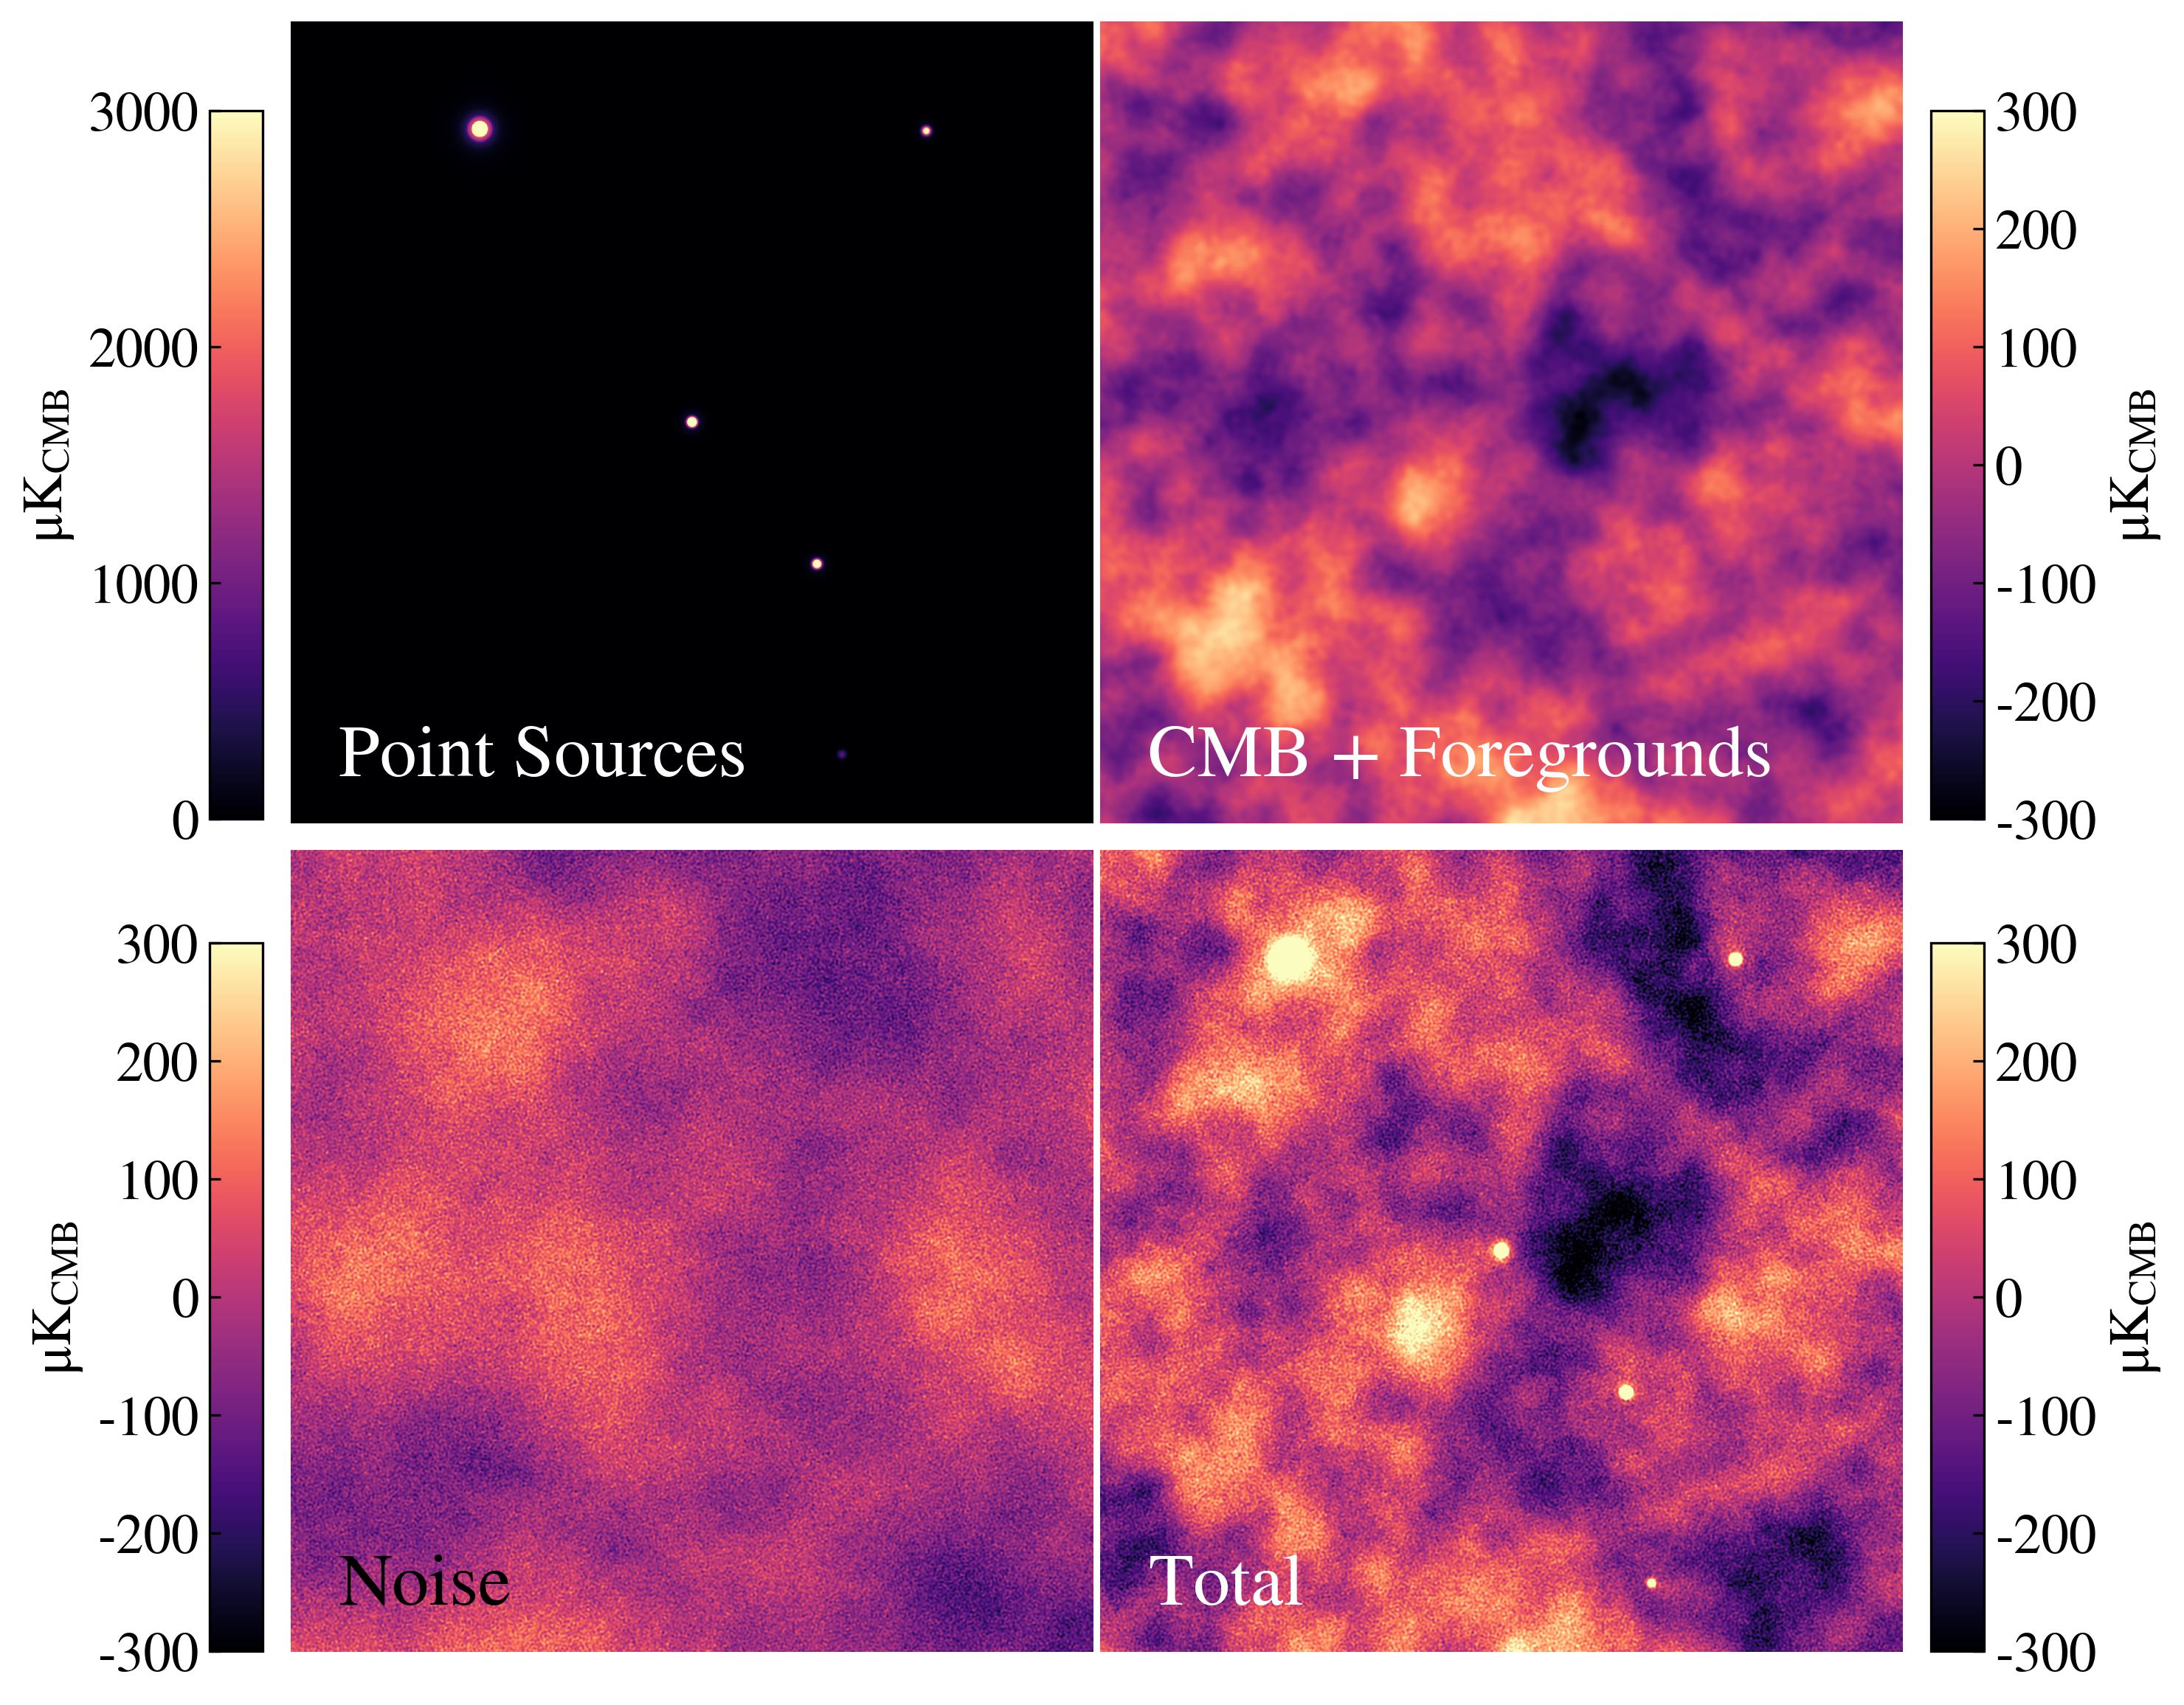
\includegraphics[width=.9\linewidth]{Figures/simmap.png}
    \caption{Example of a simulated map used to characterize the stacking bias.  This example is for PA5 in the F090, zoomed in to an area of $2\deg\times2\deg$.  Top left: Point-source map using the input catalog ra and dec coordinates.  Top right:  Simulated CMB.  Bottom left:  Simulated noise~\cite{atkins}.  Bottom right: Final simulated map after combining the previous three components.  This process is done for each PA and F-band, and repeated 100 times to estimate radial profile errors.
    }
    \label{fig:sim_map}
\end{figure*}

We simulate a stacked profile to validate our stacking pipeline and to estimate statistical uncertainty on the radial profiles presented in Section~\ref{sec:act_results}.  We first simulate a map by combining simulated point sources (referencing the catalog) along with a simulated CMB and foregrounds, and additionally adding simulated noise.  An example of a simulated map (box area of $\pm2\deg$ is shown in Figure~\ref{fig:sim_map}.  The four quadrants show the three main components of the simulated maps, followed by the total simulated map as the prior three are combined.  Here, we detail the construction of the simulations.

\subsection{Point Source Map Simulation}
\label{subsec:sim_ptsrc}
A point source map is simulated using the input catalog, and point source selection described in Section~\ref{subsubsec:cat_sel}.  The Uranus-derived beam defines the shape of the point sources in the simulated map.  Fluxes of each point source are obtained from the catalog and converted to the units of the data maps ($\mu K_\text{CMB}$) using the fiducial beam solid angle and center frequency of the passbands.

The fiducial beam profile, fluxes and coordinates are then given to the \verb|pixell.sim_objects| function that outputs a simulated point source map with matching point sources and map shape as the catalog and DR6 map. We choose to apply to the simulated map a pixel window function that matches that of the data maps for ease of comparison.

\subsection{CMB Simulation}
\label{subsec:sim_cmb}
The second component of the simulation is diffuse sky signal comprised of the CMB and (extra-)Galactic foregrounds.  This signal is critical in the simulation because the CMB is a significant source of noise in our stacked profiles at intermediate angular scales.  To accurately estimate the uncertainty and bias introduced by the inpaint-subtraction method described in Section~\ref{subsec:stacking}, we must include the CMB in our simulations.

We use the DR4 $C_\ell^{TT}$ power spectra to draw Gaussian realizations of the diffuse sky signal. An example of this simulated signal is shown in the top right of Figure~\ref{fig:sim_map}.  This simulation also contains foregrounds, which are an important contribution at high multipoles.

\subsection{Noise Simulation}
\label{subsec:sim_noise}
The third component to complete our simulated maps is noise.  The estimation of map noise is twofold: 1) a realization of the ACT map-based noise simulations at large angular scales ($\ell<5000$) and 2) a white-noise realization drawn from the per-pixel variance maps that accompany the DR6 maps.

Map-based noise simulations are fully described here~\cite{}.  Noise simulation maps include atmosphere, ACT scan strategy, and a more detailed approach to model correlated instrument noise.  An individual noise simulation is used for each individual simulated map.

As the map-based simulations at the time of this analysis only describe the noise on large angular scales ($\ell<5000$), we manually fill in the noise on small angular scales.  We then splice together two noise simulations in $\ell$-space, such that the white noise term occupies the lower $\ell$-space and map-based noise dominates the high $\ell$-space.  An example patch of the noise map is shown in the bottom left of Figure~\ref{fig:sim_map}.

\section{Results}
\label{sec:act_results}
Here, we detail the resulting temperature and temperature-to-polarization leakage beams acquired from the stacking method described above. 

\begin{figure*}[t]
    \centering
    \includegraphics[width=\textwidth]{Figures/profiles_noP_15.pdf}
    \caption{The average radial profile of the simulated observations for PA5 at 150 GHz, comparing the azimuthal averages of the input 2D beam model and the beam of the stacked point sources. 
    }
    \label{fig:profiles}
\end{figure*}

\subsection{Main Beam}
\label{subsec:mainbeam}
This section presents the temperature profiles from stacks and compares them to the existing Uranus-derived beams from Uranus. 
\subsubsection{Profiles}
\label{subsubsec:profiles}
The stacked profiles are shown in Figure~\ref{fig:profiles}.  Each profile shows the Uranus Uranus-derived beam in black, with individual arrays plotted separately.  The bottom panel shows the difference between each array's profile to the planet.
\subsubsection{Spatial Variation}
\label{subsubsec:null_mainbeam}

To study the spatial variation of point sources, we conducted a "null test" where we stacked four categories of point sources: high and low, RA and DEC.  We separate the catalog in half by considering the median RA and DEC, such that the four categories are $\text{RA}_{\text{low}}$, $\text{RA}_{\text{high}}$, $\text{DEC}_{\text{low}}$ and $\text{DEC}_{\text{low}}$. 
 Figure~\ref{fig:bells} shows the resulting window functions $B_{\ell}$ for each F-band and PA.

From this test, we find the special sources have spatial dependence where the $\text{DEC}_{\text{low(high)}}$ and $\text{RA}_{\text{high(low)}}$ match in window function, but differ from its opposite.  \textcolor{red}{Sentence explaining this effect or how it is consistent with other analyses.}
\begin{figure*}[t]
    \centering
    \includegraphics[width = \textwidth]{Figures/polbeams.png}
    \caption{Polarization leakage from stacked F150 PA4 beam, for the ML sources.  The left column shows the stacked map, the middle column is the modelled polarization leakage, and the right column is the difference between them.}
    \label{fig:polmodel}
\end{figure*}


\begin{figure*}
    \centering
    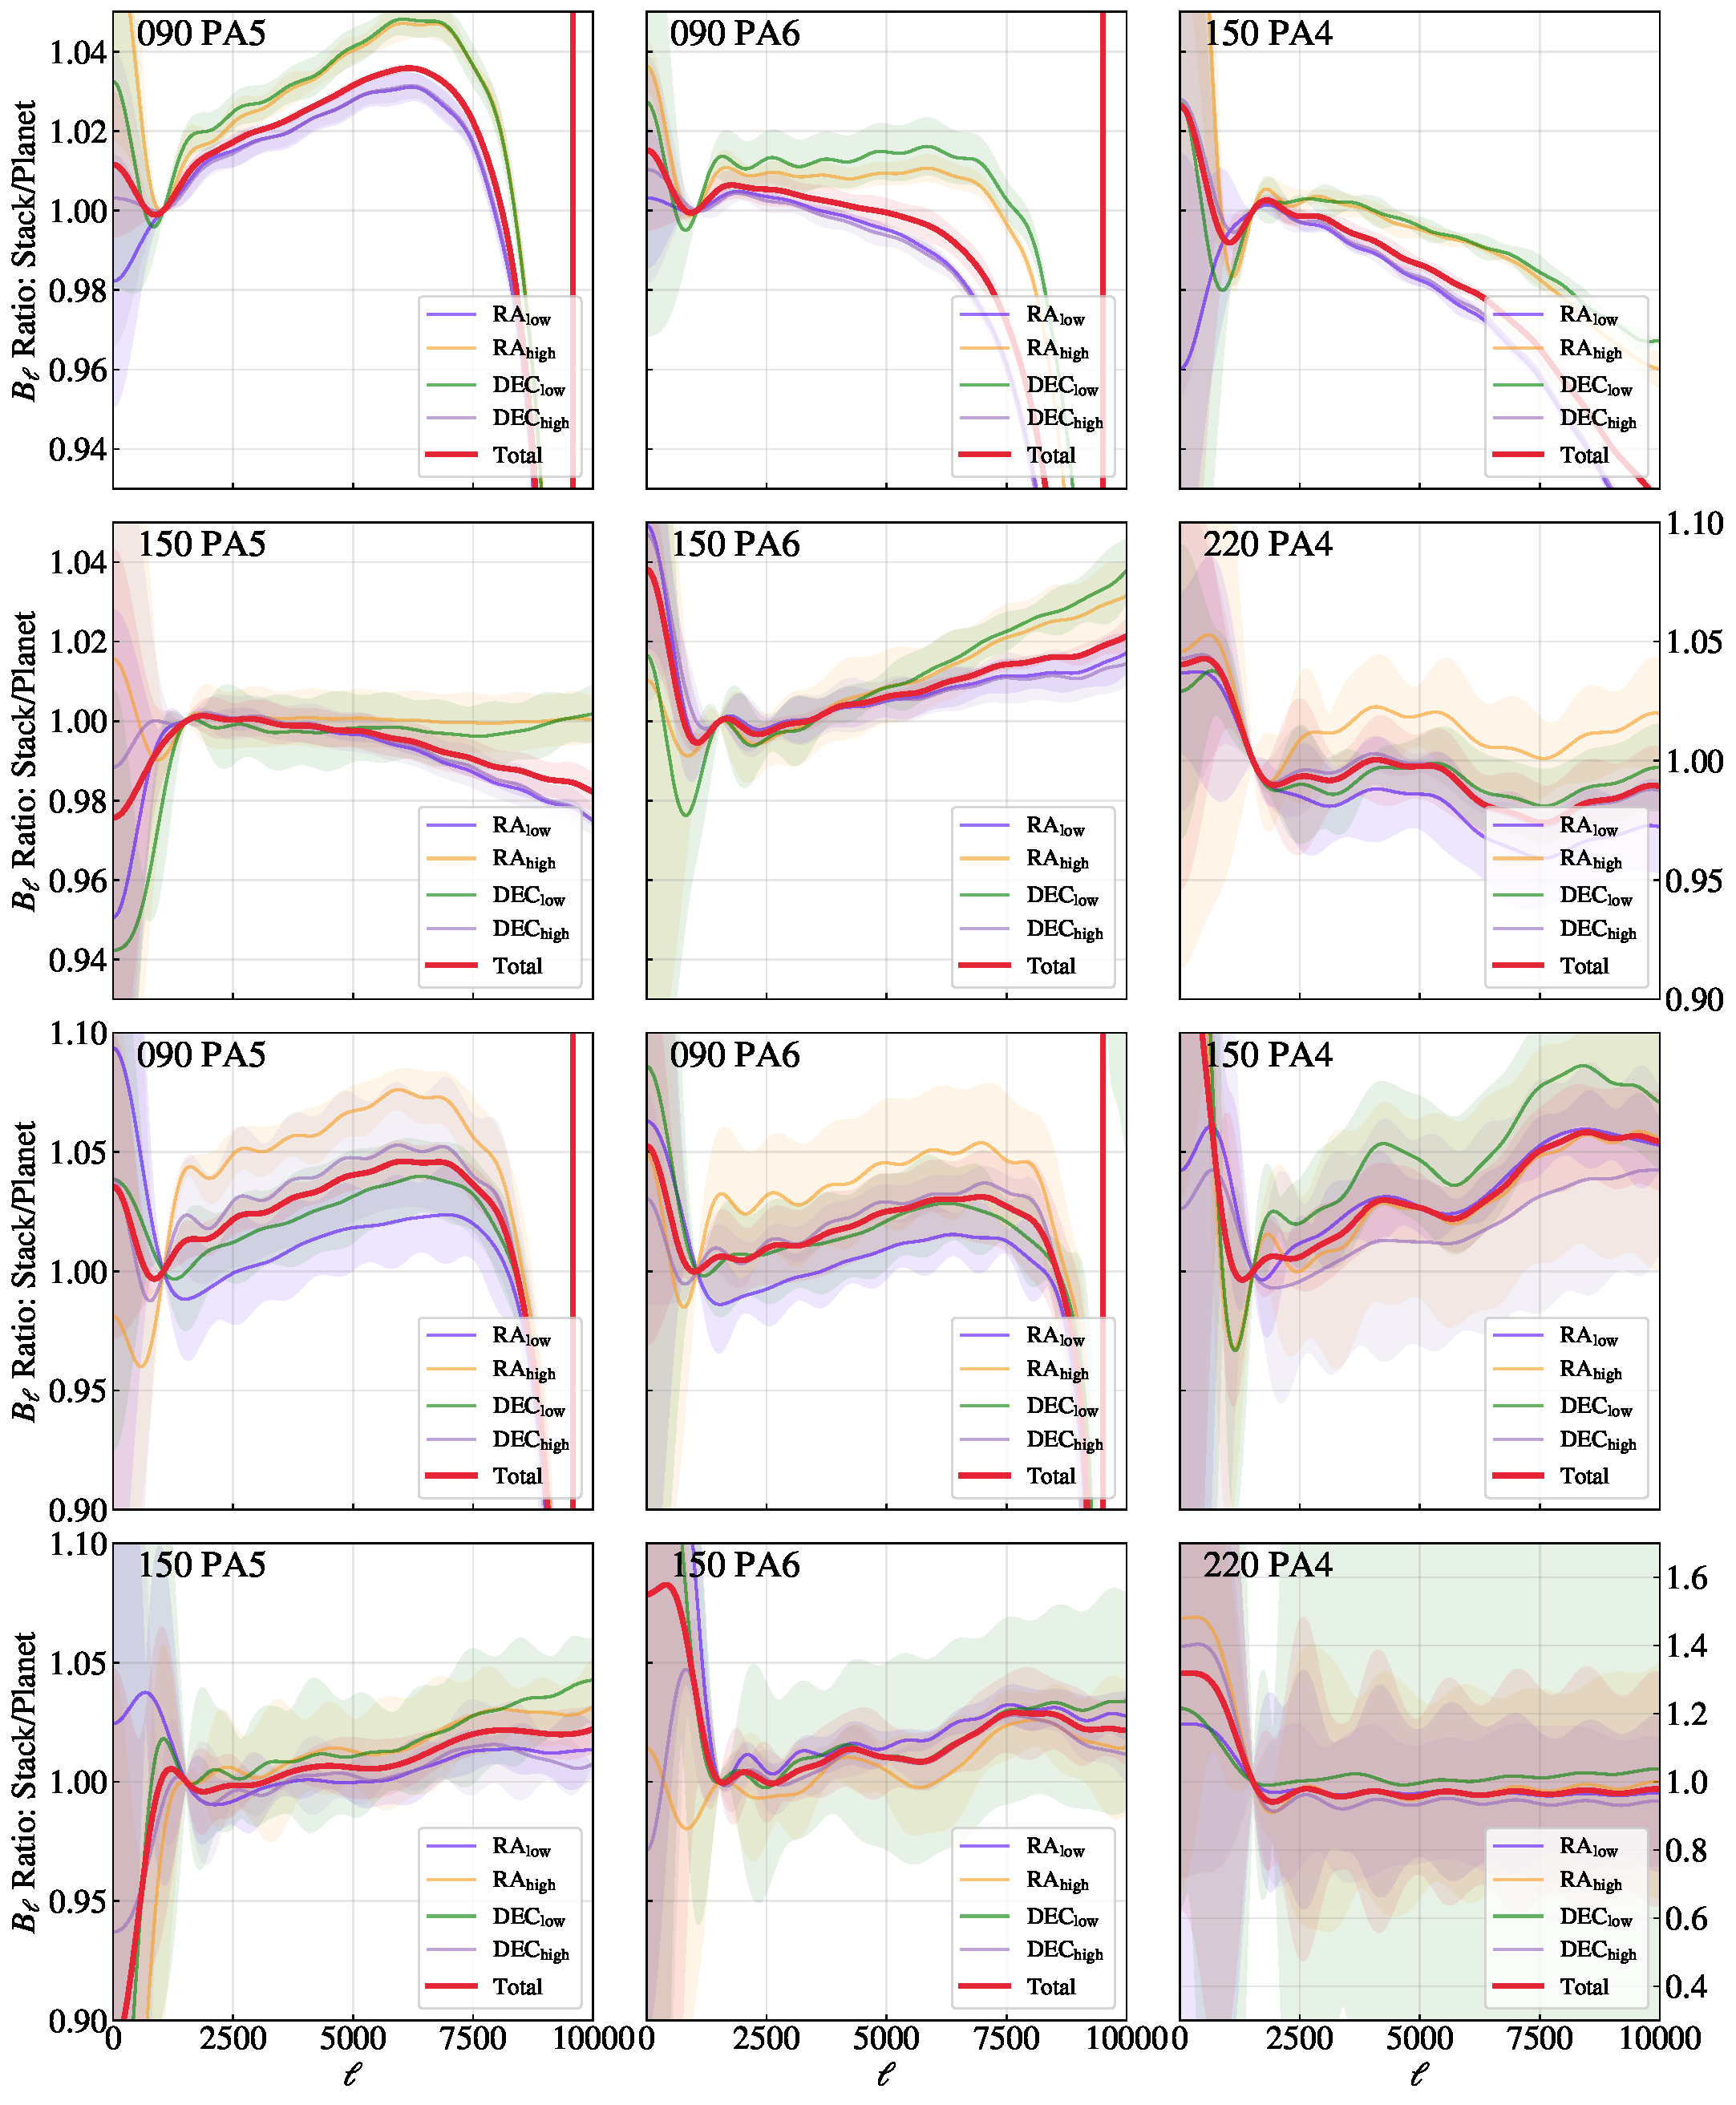
\includegraphics[width=.95\textwidth]{Figures/Bells_ratio_planet.png}
    \caption{Window function of stacked point sources, separated by RA and DEC, which we consider as a null test.  The full map stacked is plotted in red.}
    \label{fig:bells}
\end{figure*}

\subsection{Temperature to Polarization Leakage Beam}
\label{subsec:polbeam}

Here, we present the polarized beams of the stacked point sources to determine polarization leakage in the instrument.  The leakage is relatively small compared to the magnitude of the temperature beam, however the sensitivity of ACT DR6 data is such that this leakage needs to be accounted for in the analysis.  Previously, observations of Uranus were used to build an $\ell$-space T-to-P leakage function for a given frequency and array in the instrument.  Here, we test this method by comparing the leakage to our new method of stacking.
\begin{equation}
\label{eq:trans_e_b}
    \{\tilde{E}(\ell), \tilde{B}(\ell)\} = -2\pi\int \{\tilde{Q}_r(\theta),\tilde{U}_r(\theta) \} J_2(\ell\theta)\;\theta\;d\theta \; .
\end{equation}

\begin{figure*}
    \centering
    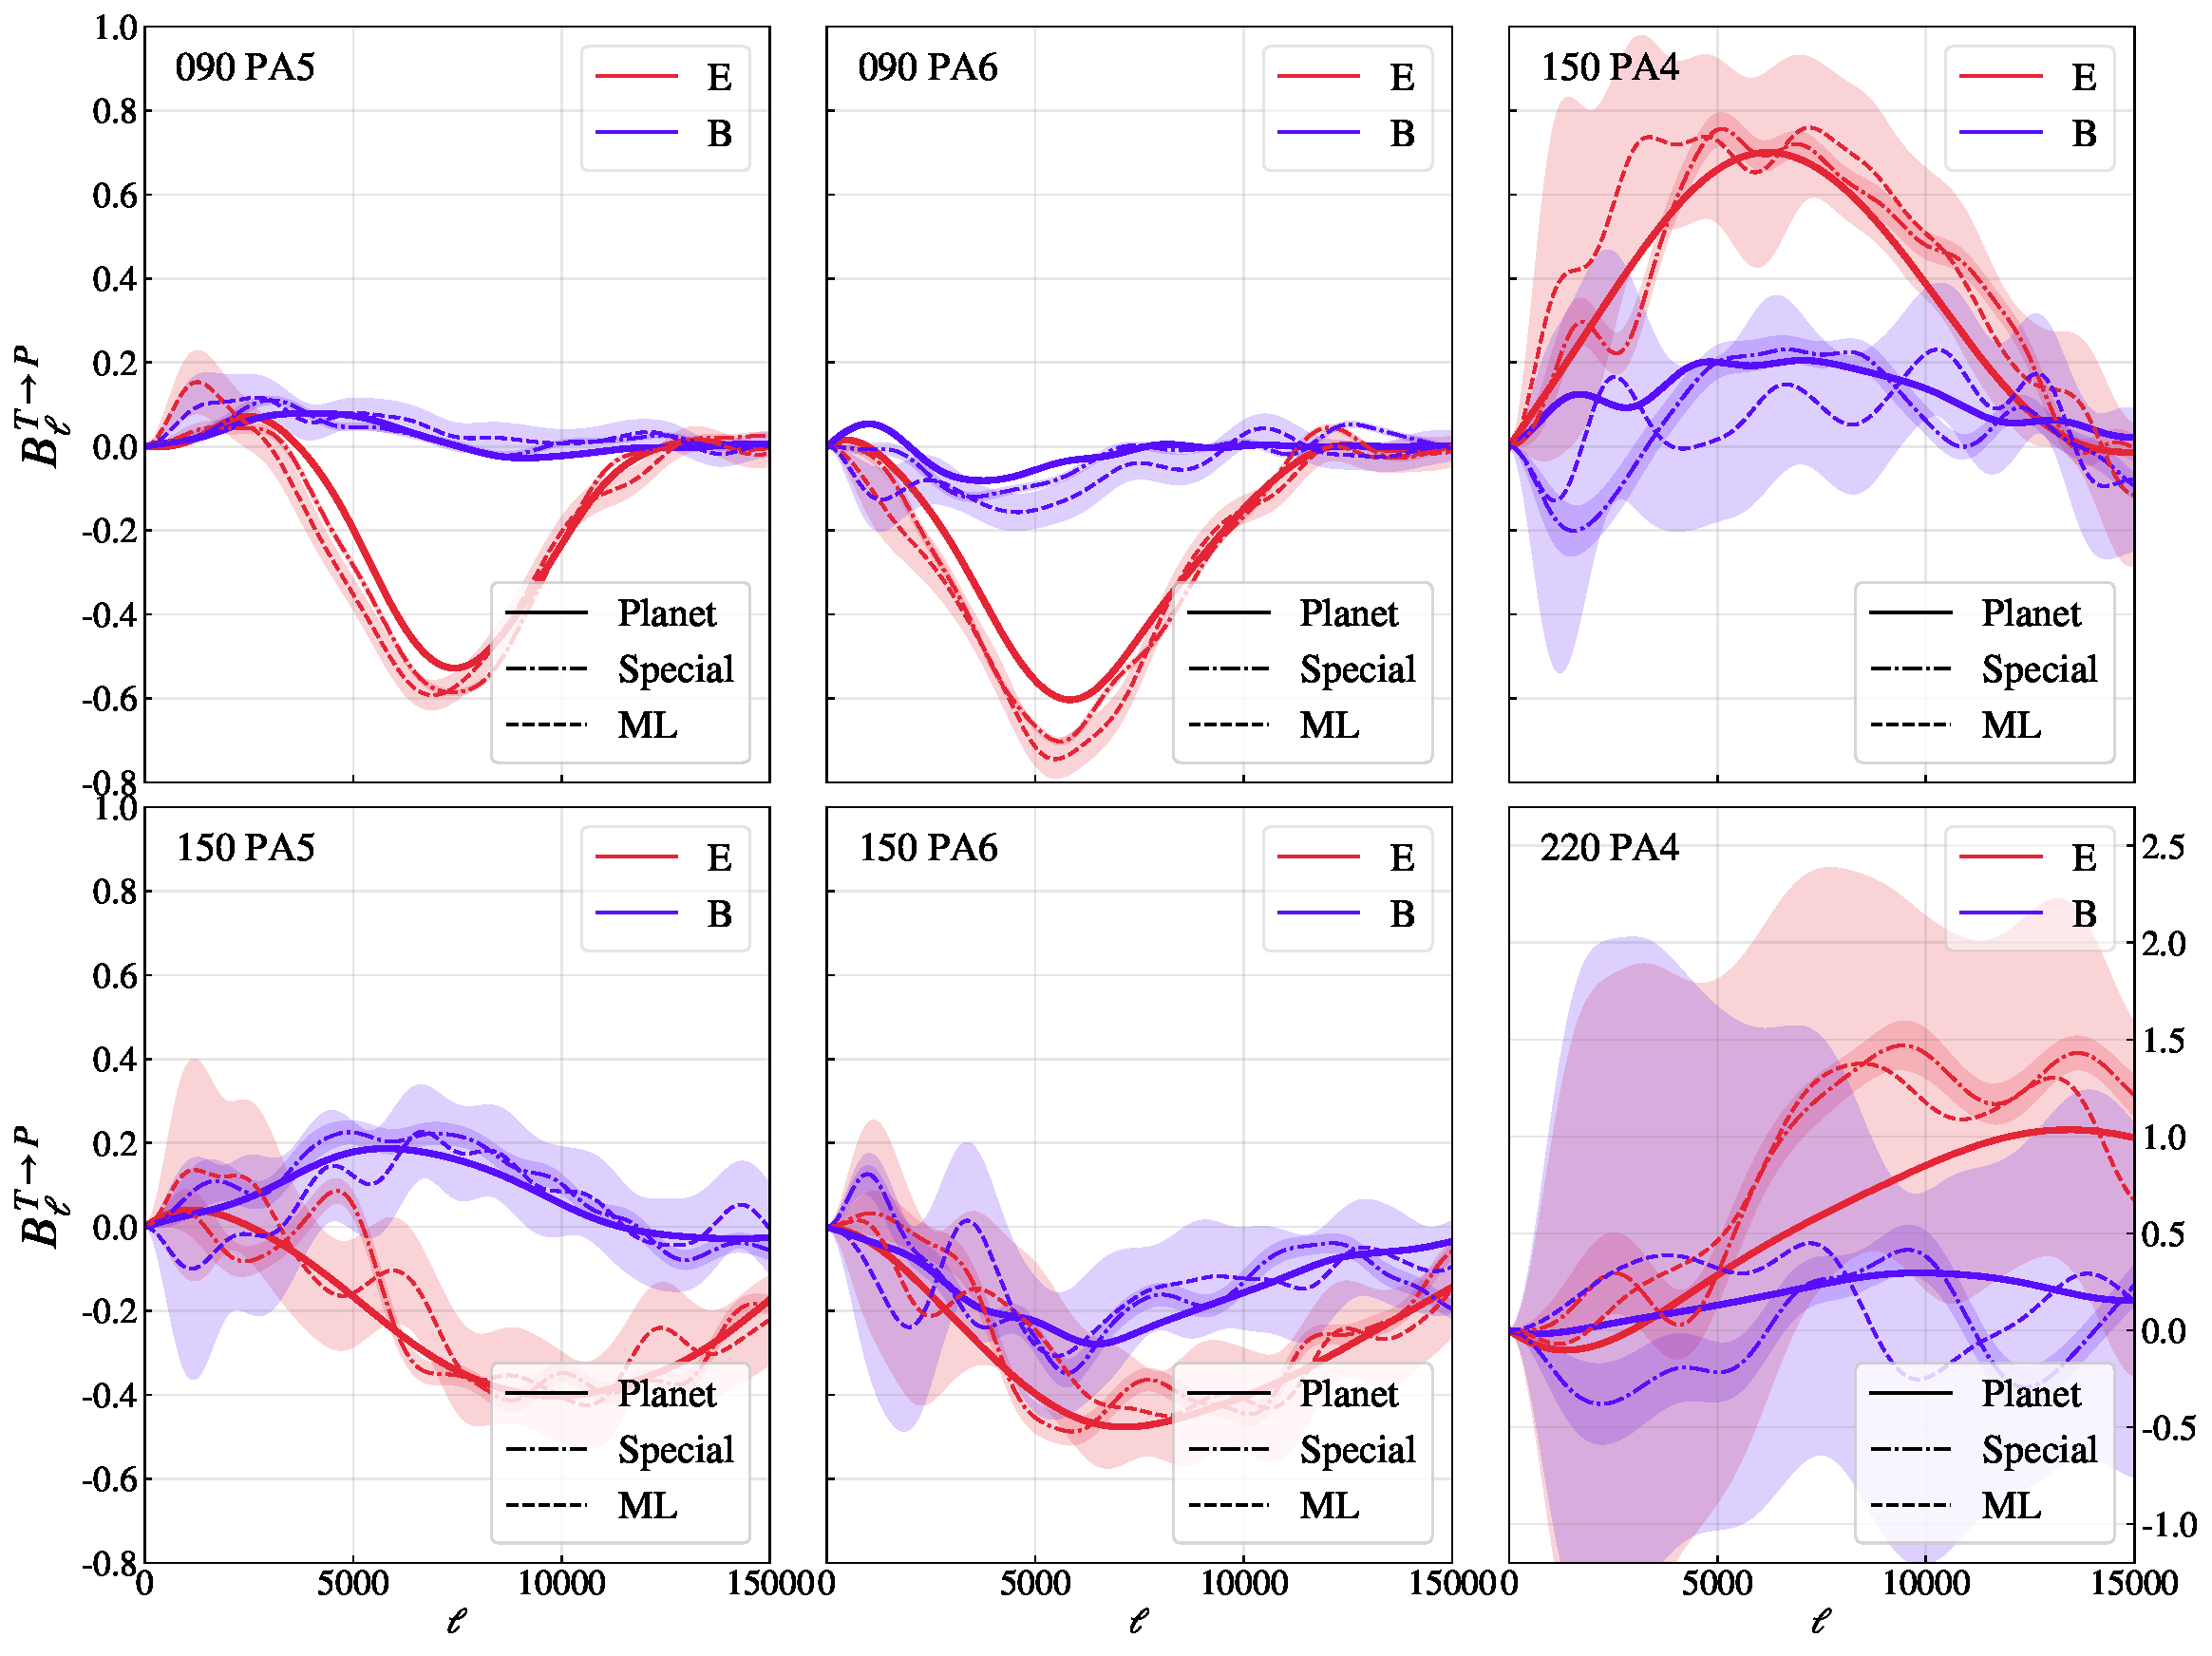
\includegraphics[width = \textwidth]{Figures/leakage.pdf}
    \caption{Polarization leakage from stacked}
    \label{fig:leakage}
\end{figure*}

Figure~\ref{fig:polmodel} shows an example of the stacked polarization leakage beam, the modelled beam, and the residual for F150 PA4.  From the window functions, we obtain the window functions of each array's T$\xrightarrow[]{}$E and T$\xrightarrow[]{}$B leakage (Figure XXX).


\section{Discussion}
\label{sec:act_disc}

\subsection{Beam Products}
\label{subsec:prods}

\subsection{Conclusion}
\label{subsec:concl}
In this paper, we have presented the analysis of the ACT beams for DR6, which includes data from 2017--19. ...
\chapter{Conclusion}
\label{ch:conclusion}
\begin{figure}[H]
    \centering
    \includegraphics[width = \textwidth]{Figures/conclusion.png}
    \label{fig:finalfigure}
\end{figure}
Experimental cosmology is in an era of precision instrumentation.  Such precision instrumentation requires understanding optical components in the telescope, careful characterization of its performance, and detailed analysis of its optical performance.  In this work, I have presented several advances in instrumentation and optics which will advance our understanding of the universe.  I have also presented novel methods for characterizing the instruments to further improve systematics. 

\section{Optical Characterization of Materials}
Understanding the optical properties of the materials within the telescope is crucial for predicting its optical performance.  This becomes even more critical as detectors increase in sensitivity; optical systematics need to be tightly constrained.
In this work, I presented the characterization of a variety of optical components for ground-based cosmological experiments.  

\subsection{Meta-material Absorbers for Stray Light}
As detector sensitivity improves, systematics must be mitigated. For example, stray light within an optics tube results in loading onto the detectors, degrading the signal-to-noise of the camera.  To control and mitigate unwanted scattering within the optical system, we develop meta-material absorbers which stop the scattering at the front of the telescope prior to entering deeper into the optics tube.  
 
As presented in Chapter~\ref{ch:mma}, we use the holography receiver to characterize the meta-material absorbers in the mid-frequency band.  We measure the reflectivity and scattering properties of the meta-material absorber, and compare its performance to alternative absorbers used in experimental cosmology.  We find he integrated scattering power is less than 1\% with the angle of incidence  $\leq45\deg$.  \textcolor{red}{Sentence about the significance of this finding...}


\subsection{Silicon Lenses}
Silicon is an optimal material for re-imaging the millimeter-wave photons onto detectors.  Its index of refraction provides fast re-imaging of the beam onto the detectors with low loss of signal.  The specific index of refraction informs the optical design of the telescope, and thus it is crucial to know the exact loss and optical properties of the lenses during the optical design.  The loss tangent is critical to constrain, as it dictates the loss of power as signal propagates through a medium.

Chapter~\ref{ch:si} reports the measured reflectivity of two silicon samples for potential use in cosmology experiments, and here are studied using a holography imaging setup.  From the reflectivity, we determine the loss-tangent of both samples, and find the "intrinsic" silicon has a lower loss-tangent than the neutron-doped silicon across the mid-frequency band (75-160\,GHz), therefore making it a better material for lenses in experimental cosmology.

\section{Characterization of the Large Aperture Telescope Receiver Tester for Simons Observatory}
Integrating and testing the optical performance of a telescope prior to deployment is novel; it is common to characterize the beam of a telescope at the site.  However, once at the site, it is nearly impossible to alter the hardware and probe its functionality.  In Chapter~\ref{ch:ot_holo}, we present the characterization of the Simons Observatory Large Aperture Telescope Receiver with radio holography.

From this optical characterization, we found a source of scattering which, when removed, improved efficiency in the mid-frequency band by roughly 5\%.  Characterizing the fully integrated optical system allowed for multiple tests and the careful discovery of additional sources of scattering prior to deployment.  We also determined the on-sky beam prior to deployment by propagating the near-field measured beams through the LAT and into the far-field, verifying the on-sky beam size was within SO's requirement.  \textcolor{red}{Sentence about the significance of this finding...}

\section{Characterization of the Small Aperture Telescope for Simons Observatory}
Following the characterization of the LAT optical system, we present preliminary results of the SAT optical system measured with the same radio holography receiver (Chapter~\ref{ch:sat_holo}).  Though results are preliminary, we determine the on-sky beam to be within 10\% of the expected beam size in the mid-frequency band.  This further demonstrates the applicability of radio-holography system to other optical systems prior to deployment.  

\section{Wavefront Optimization with Radio Holography and Machine Learning}

To enable large aperture cosmology experiments, it is common to use large reflector mirrors which are made up of many panels.  Such reflectors can create wavefront errors due to the Ruze principle.  In Chapter~\ref{ch:holosim}, we presented the SO dual reflector optical system (Large Aperture Telescope) and a method of measuring the panel offsets using radio holography paired with machine learning.  This approach can yield $<5\,\mu$m alignment errors, the requirement for SO science goals.

\section{Point Source Stacking for AdvACT}


\appendix
\chapter{Open Source Holography} % Main appendix title
\label{app:holog}

\section{Open-Source Holography}
\label{sec:appendix_hardware}

Figure~\ref{fig:setup} shows a schematic of the RF electronics.  Two local oscillators (LOs) produce signals between 10 and 13 GHz. The LO1 synthesizer produces a signal between 10 and 13\,GHz, while LO2 produces the same frequency with some offset $f_{\text{offset}}$ (this offset is chosen to be 10\,MHz).  The offset frequency is what will eventually produce an intermediate frequency exiting the mixer diplexers.  The purpose of the mixer diplexers is to ensure the signal from the first LO travels to the two mixers, and then ensures that the IF output of the mixers travels in the opposing direction down the RF chain to the FPGA.

The LO1 signal goes to the active multiplying chain, where it is multiplied by 8(12), obtaining frequencies in the F90(150)-band.  Prior to leaving the source horn, -10dB of the signal splits off, and mixes with LO2 in the harmonic mixer, producing an intermediate frequency IF$_1$ which then goes through one of the mixer diplexers and to the FPGA.  The rest of the signal leaves the source horn, through the components of the LATR optics, and the signal reaching the back of the optics tube mixes with LO2 in a GaAs harmonic mixer, and the subsequent intermediate frequency, IF$_2$, which also travels to the FPGA.  The FPGA used for these measurements is the Re-configurable Open Architecture Computing Hardware (ROACH-2) board, which correlates the reference and modulated signals~\cite{roach2}.

\begin{figure}[ht]
    \centering
    \includegraphics[width = \textwidth]{Figures/FPA.jpeg}
    \caption{The Simons Observatory Large Aperture Telescope optics tube focal plane readout, which is cooled to 4\,K during measurements.  The holography receivers (two receivers for redundancy) are approximately 7.4\,cm from the center of the focal plane.}
    \label{fig:fpa}
\end{figure}

The signal from the source(receiver) needs to be amplified due to high loss levels in the coax path from the harmonic mixer on the source to the reference mixer-diplexer (LATRt readout chain).  To overcome this loss, amplifiers with attenuators  increase the signal in the RF chain prior to entering the mixer diplexer.  The setup uses low phase variation coaxial cables leftover from the DASI experiment~\cite{CHURCH20031083}.  The phase repeatability of the holography setup is within $\approx3^{\circ}$.  We further note that any drift in the map would present itself in the phase map.  This phase drift would be removed during the propagation into the far-field when we optimize the position of the beam map in the LAT focal plane. 

The source moves in a 2-D grid above the LATRt with motorized XY stages~\cite{stages}.  The source mounts to the stages such that the signal points downwards towards the LATRt window.  The laboratory is over 7.5\,m tall, and therefore we expect reflection from the walls to be diffuse.  Therefore, the reflected signal is diluted before reflecting into the testing system.  The dominant reflections are from reflections within the optics tube, as the hexagon side-lobe is the dominant side-lobe feature in the beam maps (Figure~\ref{fig:beam_measurements_all}).
Figure~\ref{fig:fpa} shows the holography receiver readout at the back of the optics tube focal plane.  An SO MF feedhorn array is adapted for the holography experiment.  On the readout side of the array, attachment screws are added for attaching a circular to rectangular transition waveguide.  The transition waveguide connects the back of the focal plane (circular) to the GaAs W-band harmonic mixer (rectangular).  Though the design of the W-band harmonic mixer is optimized for F90 frequency readout, the W-band harmonic mixer is used for both F90 and F150 measurements (the entire SO MF band), allowing for a wider band of measurements without separate LATRt cool-downs.
\begin{figure*}[t!]
    \centering
    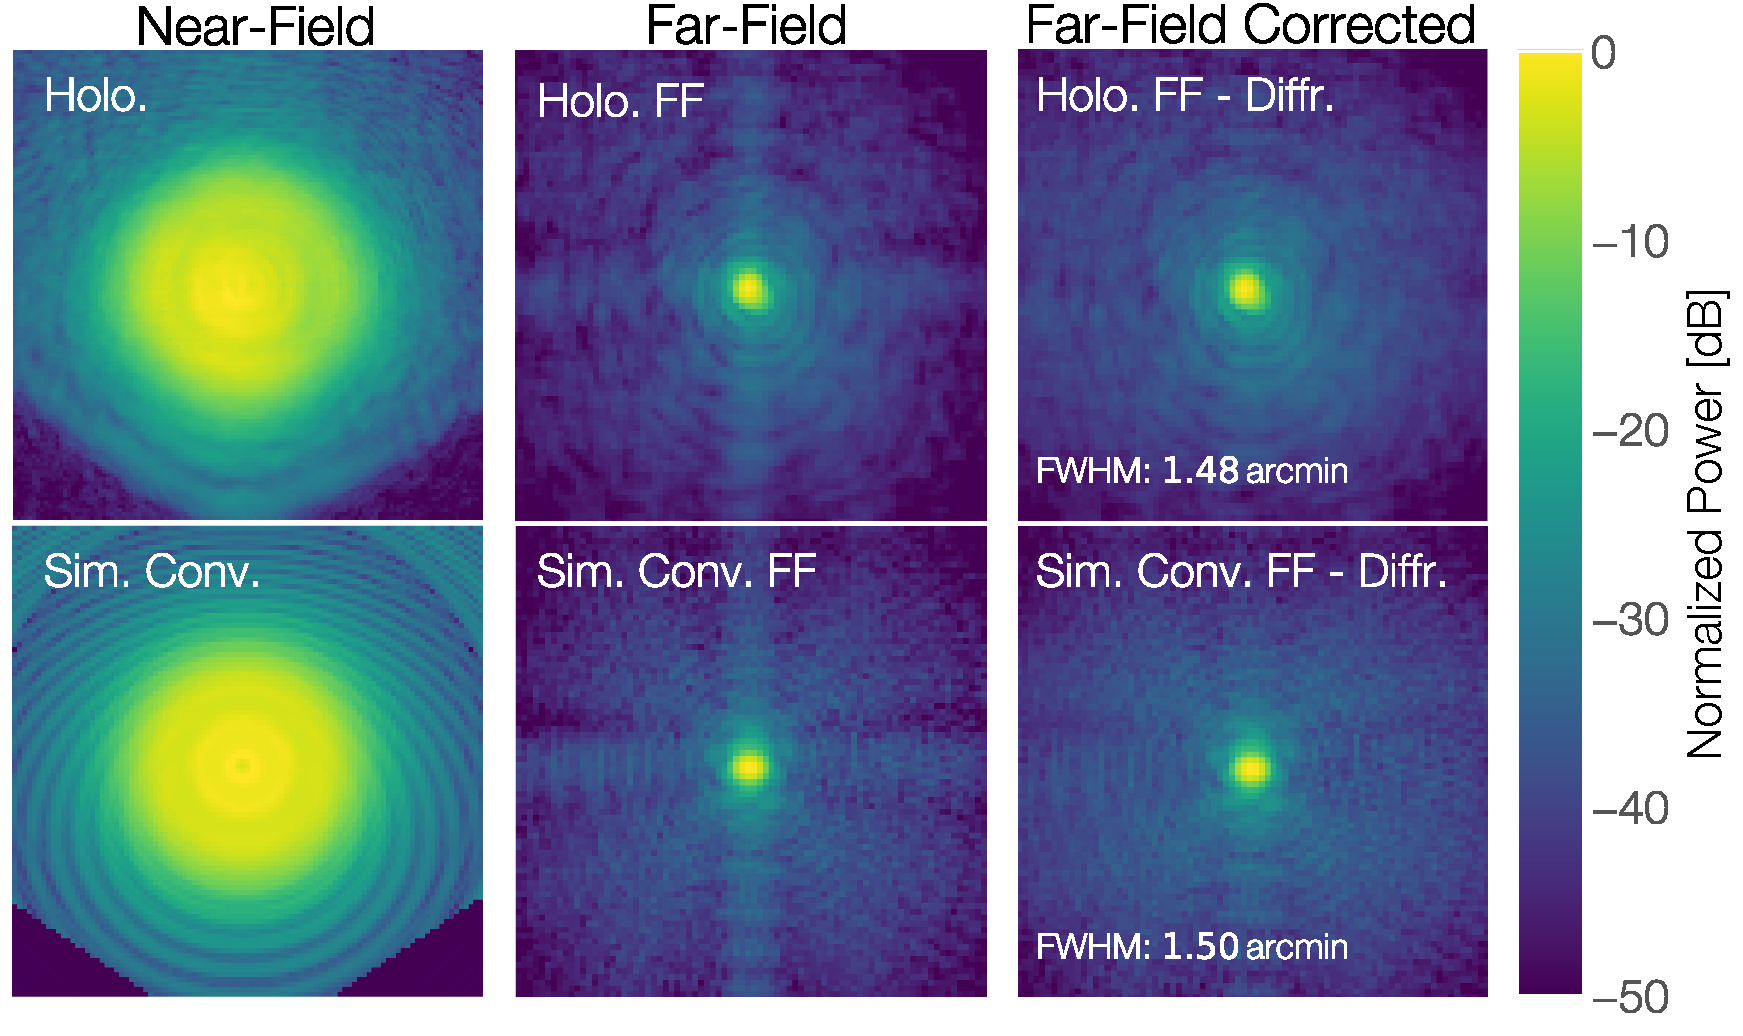
\includegraphics[width = \textwidth]{Figures/forward_convolve_highres.pdf}
    \caption{Forward modelling method with the F150 band-averaged holography data. Column 1:  Near-field holography data(top) and convolved simulation with a scattering term(bottom).  Square is $12\times12\,$cm.  Column 2: Far-field holography data(top) and convolved simulation with a scattering term(bottom).  Diffraction spikes consistent with a convolution from a square aperture are present in both the measured far-fields and the simulated far-fields, due to the source horn having a rectangular aperture face.  Square is $20\times20\,$arcmin.  Column 3:  Far-field holography data with diffraction model removal(top) and convolved simulation with a scattering term with diffraction model removal(bottom). Square is $20\times20\,$arcmin.}
    \label{fig:forward_model}
\end{figure*}
\section{Forward Modelling}
\label{sec:forward_model}
\begin{figure*}[t]
    \centering
    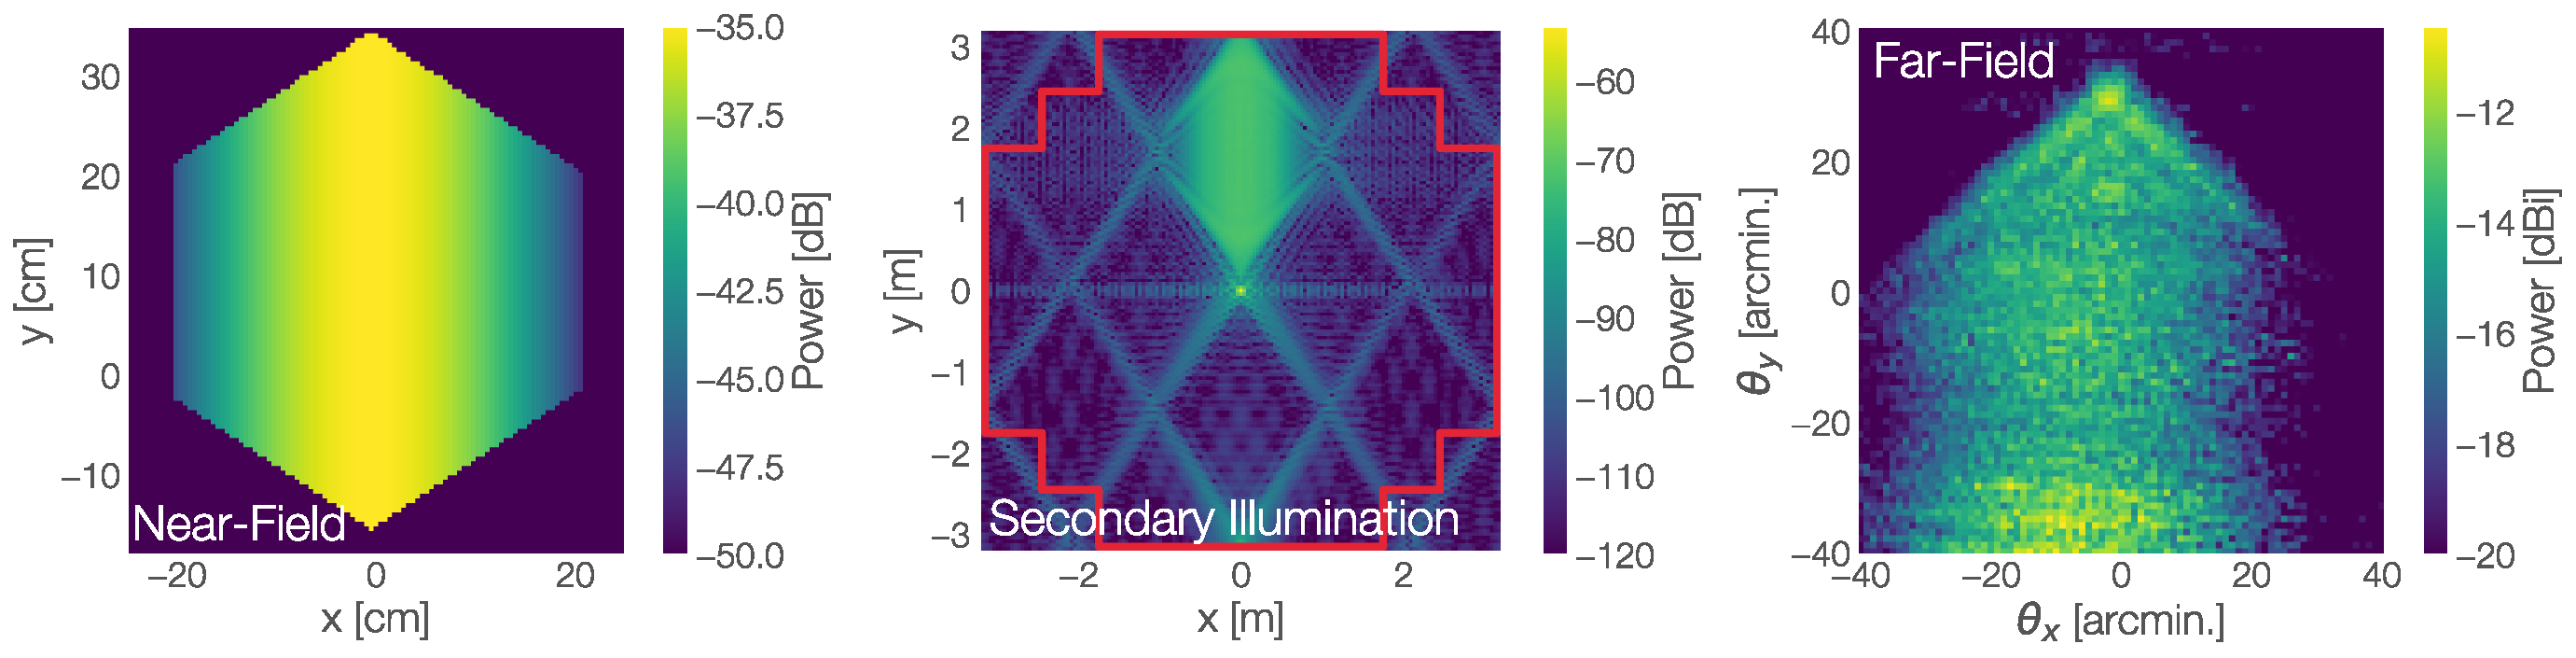
\includegraphics[width = .95\textwidth]{Figures/scatter_model.pdf}
    \caption{Simulated scattering term (power) in the near-field(left), at the secondary illumination(middle) and propagated to the far-field(right).  Each subplot is the band-averaged simulation over all F150 frequencies.}
    \label{fig:scattering_forward}
\end{figure*}
As introduced in Section~\ref{sec:results}.~\ref{sec:prop_fields}, the holography source emits from a rectangular feedhorn, and therefore result in a convolution of the electromagnetic field from the optics tube with the field pattern on the feedhorn aperture.  Convolving the simulated fields increases the F90(150) far-field beam by 12.2(4.7)\% and results in horizontal and vertical diffraction spikes in the raw far-field calculation~\cite{Goodman2005-ne}.

We carry out the forward modelling by building a simulation of the optics tube beam pattern at the measurement plane.  This model includes an empirical model of the scattering of the optics tube with the hexagonal outline to model the boundary of the optics tube window, and a similar amplitude and phase to what is measured.  The resulting simulated F90(150) beam matched the measured FWHP beam width within in 1.73(0.7)\%.  The simulation also had the horizontal and vertical diffraction spikes in the far-field due to the impact of the convolution with the holography source feed pattern~\cite{Goodman2005-ne}.  The full forward modelling process is shown in Figure~\ref{fig:forward_model}.

For visualization purposes, these spikes are removed by subtracting a model $D(\theta_x,\theta_y)$ (amplitude of the electric field) consisting of a $\sinc$ function with a Gaussian width along its narrow direction equal to the beam width (Eq.~\ref{eq:model_conv}), where $\theta_x$ and $\theta_y$ are elevation and azimuth, and we fit the 2 parameters $\sigma_{\theta_x}$ and $\sigma_{\theta_y}$.  This model is based on the predicted Fraunhofer diffraction pattern from a rectangular aperture~\cite{Goodman2005-ne} (e.g., the feed) and was shown to match the simulations.
\begin{equation}
    D(\theta_x,\theta_y) = \exp^{-(\theta_x^2/4\sigma_{\theta_x}^2 +\theta_y^2/4\sigma_{\theta_y}^2 )}\sinc{\theta_x}\sinc{\theta_y}
    \label{eq:model_conv}
\end{equation}
The holography measurements showed scattering from within the optics tube (hexagonal shape at ~-20\,dB in Figure~\ref{fig:beam_measurements_all}).  To understand how this scattering propagates through the telescope, we add a scattering term (with both amplitude and phase) to the simulated beam, and then propagate this beam into the far-field.  We also investigate how the side-lobes measured outside the main beam (Fig.~\ref{fig:beam_measurements_all}) propagate into the far-field (Fig.~\ref{fig:scattering_forward}).  Reflections are known to be a problem in near-field beam mapping~\cite{2020JLTP..199..156Y,7740846,387181}.  However, the inferred amplitude of the probe is small, and we do not correct for reflections.  The side-lobe spreads out and is localized to 2 meters from the center of the primary and secondary mirrors, and then leads to a $0.85^{\circ}$ diffuse structure on the sky that is at the $\approx -15$\,dBi level.

\section{Measurement Requirements}
\label{sec:err_prop}
Here, we discuss the measurement requirements to meet specific far-field grid resolution and range from near-field data.  Near-field beams with three signal-to-noise levels are propagated into the far-field (for 90\, and 150\,GHz near-field beams); we simulate the near-fields to have 20, 40, and 60\,dB signal-to-noise.  The signal-to-noise propagated to the secondary illumination and far-field is listed in Table~\ref{tab:fft_sn}. 

\begin{table}[ht]
\centering
\begin{tabular}{|c|c|c|c|c|}
\hline
F\,[GHz] & \multicolumn{3}{c|}{S/N [dB]}\\
& NF& Sec.& FF\\
\hline
 90      
         & 20& 21.7 & 40.0 \\
         & 40& 37.0 & 43.9 \\
         & 60& 45.4 & 43.9 \\
 150     
         & 20& 18.0 & 39.3 \\
         & 40& 35.5 & 43.8 \\
         & 60& 46.0 & 43.8 \\
 \hline
\end{tabular}
\caption{Near-field simulated measurement signal-to-noise and resulting simulated side-lobe power (at the secondary illumination and into the far-field).  Signal-to-noise is calculated as the standard deviation of the signal outside an 8.5\,cm radius of the peak-normalized beam (same resolution as Table~\ref{tab:fft_grid}).}
\label{tab:fft_sn}
\end{table}

When planning the near-field scan, we consider the resolution and how the near-field grid propagates into the plane of the secondary, due to the Fourier relationship between near- and far-fields (Eq.~\ref{eq:fft}), and into the telescope's far-field through the modeling described in Section~\ref{sec:prop_fields}. Table~\ref{tab:fft_grid} summarizes the scan size and resolutions and resulting far-field size and resolution grids used in the holography measurements presented here.
\begin{table}[htb]
\centering
\begin{tabular}{|c|c|c|c|c|c|c|}
\hline
F\,[GHz] & \multicolumn{2}{c|}{NF [cm]}&\multicolumn{2}{c|}{Sec. [m]} & \multicolumn{2}{c|}{FF [arcmin]} \\
 & Size & Res. & Size & Res.& Size & Res.\\ \hline
 90 & 50& 0.25 & 9.52& 0.13& 119.72 & 0.60\\
 150 & 50& 0.20 &6.66 &0.06 &128.40&0.52\\
 \hline
\end{tabular}
\caption{Near-field scan size and resolution, and resulting scan size and resolution at the secondary illumination and in the far-field.}
\label{tab:fft_grid}
\end{table}
When planning the near-field scan, we consider the resolution and how the near-field grid propagates into the far-field, due to the Fourier relationship between near- and far-fields (Eq.~\ref{eq:fft}).  Table~\ref{tab:fft_grid} summarizes the scan size and resolutions and resulting far-field size and resolution grids used in the holography measurements.

\chapter{Holography Receiver Polarization Through the Large Aperture Telescope Optics Tube} 
\label{app:pol} 
Using the holography experiment, we obtain measurements for the cross-polarization of the LATR tester, including holography linearly polarized source, dielectric polarizing grid, optics tube, and holography receiver.  In order to model the polarization response in the setup, we employ Mueller matrix math to modulate the Stokes parameters of the signal throughout the setup.  

Here, we derive each component of the polarization modulation using Mueller matrix notation~\cite{MUELLER}.  This model is then fit to the measured response through the polarized grid in the LATR tester optics tube, using the same holography receiver.  The power measured by the detector $P_{d}$ can be modelled as a series of polarization modulations: 
\begin{equation}
    P_{\text{d}}(\theta) = \vec{S}_{d}(\phi_{d},\epsilon)\cdot \vec{M}_{\text{OT}}\cdot \vec{M}_{g}(\theta,\eta_{g})\cdot \vec{S}_{s}
    \label{eq:holo_model}
\end{equation}
where the source emits the Stokes parameters $\vec{S}_{s}$, which is then modulated by the grid $\vec{M}_{g}$.  The field then enters the optics tube $\vec{M}_{\text{OT}}$ and is measured by the detector $\vec{M}_{d}$.  These data were used to quantify the grid efficiency $\eta_{g}$, the cross-polarization of the instrument $\epsilon$ (this can be complex), and the tilt-offset of the holography detector $\phi_{d}$.  We are fitting our data to this model, where we fit the 3 parameters $\epsilon$, $\eta_{g}$, and $\phi_{d}$.
\section{General Notation}
\subsection{Stokes Parameters}
First, let's define our basis of Stokes parameters and how they physically relate to our setup.  The Stokes parameters are:
\begin{equation}
\begin{split}
    I & = |E_x|^2 + |E_y|^2 \\
    Q & = |E_x|^2 - |E_y|^2 \\
    U & = E_x E_y^* + E_x^*E_y\\
    V & = i(E_x E_y^* - E_x^*E_y) \\
\end{split}
\end{equation}
\subsection{Jones into Mueller Matrix}
To derive the model, we employ Mueller matrix notation.  We often start by modeling a component by its Jones matrix, then converting to its Mueller matrix to interact with the Stokes parameters of the setup. Therefore, here I review this conversion.  Converting the Jones matrix $J$ to Mueller matrix $M$:
\begin{equation}
    M = A(J\otimes J^*)A^{-1}
\end{equation}
with the $A$ matrix:
\begin{equation}
    A = \begin{bmatrix}
    1 & 0 & 0 & 1\\
    1 & 0 & 0 & -1\\
    0 & 1 & 1 & 0\\
    0 & -i & i & 0\\
  \end{bmatrix}\quad\text{and}\quad 
     A^{-1} = \frac{1}{2}\begin{bmatrix}
    1 & 1 & 0 & 0\\
    0 & 0 & 1 & i\\
    0 & 0 & 1 & -i\\
    1 & -1 & 0 & 0\\
  \end{bmatrix}
\end{equation}
\subsection{Rotation}
We often need to convert our Stokes parameter matrix into an instrument's local coordinate system in order to determine how that instrument will modulate our signal.  Therefore, we will often use the rotation matrix:
\begin{equation}
   M_{\text{rot}}= \begin{bmatrix}
    1 & 0 & 0 & 0 \\
    0 & \cos{2\theta} & \sin{2\theta} & 0 \\
    0 & -\sin{2\theta} & \cos{2\theta} & 0  \\
    0 & 0 & 0 & 1
    \end{bmatrix}
\end{equation}
\section{Mueller Matrices}

Here we list the individual matrices which make up the full model of the measurement.  We use Mueller matrices to modulate the polarization of the holography source $\vec{S}_{co,cr}$.  

\subsection{Polarized Source}
The Stokes parameters of a general polarized source are expressed by a matrix $\vec{S}$:
\begin{equation}\vec{S} = 
    \begin{bmatrix}
    I & Q & U & V
    \end{bmatrix}^T
\end{equation}
The holography source, specifically, is linearly polarized (TM-mode) (meaning we only include the $I$ and $Q$ Stokes parameters).  The Stokes parameters of a linearly polarized source along the $\theta=0^\circ$ axis:
\begin{equation}\vec{S}_{co} = 
    \begin{bmatrix}
    1 & 1 & 0 & 0
    \end{bmatrix}^T
\end{equation}
The second source polarization was obtained by adding a waveguide twist directly onto the source's output, prior to the rectangular horn.  Therefore, the Stokes parameters of the source in the $\theta=90^\circ$ axis is modeled as:
\begin{equation}\vec{S}_{cr} = 
    \begin{bmatrix}
    1 & -1 & 0 & 0
    \end{bmatrix}^T
\end{equation}
\subsection{Polarizing Grid}
The signal is first modulated by the polarized grid prior to entering the optics tube.  The purpose of the grid is to transmit one polarization and reflect the other.  However, in the case of an imperfect polarizing grid, some of the $2^{nd}$ polarization may also transmit (a fraction of the $1^{st}$ polarization).  Therefore, we define the Jones matrix as the following, where the majority of the signal along the $x$-axis is transmitted ($t_x > t_y$):
\begin{equation}
    J_{g} = \begin{bmatrix}
    t_x & 0 \\
    0 & t_y\\
  \end{bmatrix}
\end{equation}
where $t_x\approx 1$ and $t\approx 0 $.  Now, as before, we convert to the grid's Mueller matrix:
\begin{equation}
    M_{g} =\frac{1}{2} \begin{bmatrix}
    |t_x|^2 + |t_y|^2 & |t_x|^2 - |t_y|^2 & 0& 0\\
    |t_x|^2 - |t_y|^2 & |t_x|^2 + |t_y|^2& 2\Re{(t_x t_y^*)}& -2\Im{(t_x t_y^*)}\\
    0 & 0& 2\Im{(t_x t_y^*)}& 2\Re{(t_x t_y^*)}\\
  \end{bmatrix}
\end{equation}
The efficiency of our wire grid is defined by the transmission through the $x$-axis $t_x$. We want to determine the grid efficiency from our data, so we can re-write our Mueller matrix as:
\begin{equation}
    M_{g} =\frac{1}{2} \begin{bmatrix}
    1 & \eta_g & 0& 0\\
    \eta_g & 1& 1-\eta_g^2 & -\sqrt{1-\eta_g^2}\\
    0 & 0& \sqrt{1-\eta_g^2}& \sqrt{1-\eta_g^2}\\
  \end{bmatrix}
\end{equation}
Lastly, we rotate the grid via the $M_{\text{rot}}(\theta)$ matrices:
\begin{equation}
    M_{g}(\theta,\eta_{g}) = M_{\text{rot}}^T(\theta) \cdot M_{g}(\eta_{g})\cdot M_{\text{rot}}(\theta)
\end{equation}
\subsection{Generic Instrument}
\begin{equation}
    J = \begin{bmatrix}
    1 & 0 \\
    0 & A e^{i\phi}\\
  \end{bmatrix}
\end{equation}
Converting this to a Mueller matrix yields:
\begin{equation}
    M_{\text{IP}} = \frac{1}{2}\begin{bmatrix}
    1+A^2 & 1-A^2 & 0& 0\\
    1-A^2 & 1+A^2 & 0& 0\\
    0 & 0 & 2A\cos\phi & 2A\sin\phi\\
    0 & 0 & -2A\sin\phi & 2A\cos\phi
  \end{bmatrix}
\end{equation}
We define the instrument's polarization as $\lambda_P = \frac{1}{2}\sqrt{1-A^2}$.  Here's we only consider $\phi=0$ or else we would find $A<1$, which isn't physical in our setup.  Our Mueller matrix becomes:
\begin{equation}
    M_{\text{IP}} = \frac{1}{2}\begin{bmatrix}
    1-\lambda_P & \lambda_P & 0& 0\\
    \lambda_P & 1-\lambda_P & 0& 0\\
    0 & 0 & \sqrt{1-2\lambda_P} & 0\\
    0 & 0 & 0 & \sqrt{1-2\lambda_P}
  \end{bmatrix}
\end{equation}
Our model for instrument polarization is aligned along a specific axis, so we need to rotate this matrix into the appropriate local coordinate system via the rotation matrix $M_{rot}$.
\subsection{Detector}
We model the detector as an imperfect polarizer, to include any small cross-polarization from the receiver:
\begin{equation}
    J_{d} = \begin{bmatrix}
    1 & 0 \\
    0 & \epsilon\\
  \end{bmatrix}
\end{equation}
where $\epsilon = \epsilon_0(\cos\delta + i\sin\delta)$.  The Mueller matrix then becomes:
\begin{equation}
    M_{d} = \frac{1}{2}\begin{bmatrix}
    1+\epsilon_0^2 & 1-\epsilon_0^2 & 0 & 0\\
    1-\epsilon_0^2 & 1+\epsilon_0^2 & 0 & 0\\
    1 & 0 & 2\epsilon_0\cos\delta & 2\epsilon_0\sin\delta\\
    1 & 0 & -2\epsilon_0\sin\delta & 2\epsilon_0\cos\delta\\
  \end{bmatrix}
\end{equation}
To simplify this down to one parameter, we define $\epsilon_0^2 = \chi$.  We rewrite our Mueller matrix then as:

\begin{equation}
    M_{d} = \frac{1}{2}\begin{bmatrix}
    1+\chi & 1-\chi & 0 & 0\\
    1-\chi & 1+\chi & 0 & 0\\
    1 & 0 & 2\sqrt{\chi} & 0\\
    1 & 0 & 0 & 2\sqrt{\chi}\\
  \end{bmatrix}
\end{equation}
Because the power out from the detector $P_{\text{out}}$ is the $I$ component of the Stoke's parameters, we then get the final $\vec{S}_{\text{out}}$ with:
\begin{equation}
    \vec{S}_{d} = \begin{bmatrix}
    1 & 0 & 0 & 0
  \end{bmatrix} \cdot M_{d} \cdot M_{\text{rot}}(\phi)
\end{equation}

% \chapter{Polarized Beam Transformation Formalism} % Main appendix title
\label{app:act} 

Here, we derive the locally defined map-space polarization basis to determine the polarized $\ell$-space beams from the $Q$ and $U$ beams.  The basis of $Q_r$ and $U_r$ are defined as local linear combinations of the $Q$ and $U$ maps as:
\begin{equation} \label{eq:q_r}
\begin{split}
    Q_r(\boldsymbol{\theta}) =& Q(\boldsymbol{\theta}) \cos 2\phi_{\theta} + U(\boldsymbol{\theta}) \sin 2\phi_{\theta} \\
    U_r(\boldsymbol{\theta}) =& U(\boldsymbol{\theta}) \cos 2\phi_{\theta} - Q(\boldsymbol{\theta}) \sin 2\phi_{\theta}
\end{split}
\end{equation}
where $\boldsymbol{\theta} \equiv (\theta,\phi_\theta)$ are standard polar coordinates with the beam's center as their origin and $\phi_{\theta}$ increasing clockwise from the positive $y$-axis (assuming $+x$ points to the right and $+y$ points upward).  We can also define these fields conversely:
\begin{equation} \label{eq:q}
\begin{split}
    Q(\boldsymbol{\theta}) =& Q_r(\boldsymbol{\theta}) \cos 2\phi_{\theta} - U_r(\boldsymbol{\theta}) \sin 2\phi_{\theta} \\
    U(\boldsymbol{\theta}) =& U_r(\boldsymbol{\theta}) \cos 2\phi_{\theta} + Q_r(\boldsymbol{\theta}) \sin 2\phi_{\theta} \; .
\end{split}
\end{equation}
In order to determine beam leakage in the angular power spectra, we need to translate the polarized beams $Q_r$ and $U_r$ to the $\ell$-space $E$ and $B$ polarized beams.  To do so, we employ the relation between the azimuthally averaged versions of each component, derived here in the flat-sky limit.  The Fourier-space expressions for $E$ and $B$ are:
\begin{equation} \label{eq:e}
\begin{split}
        E(\boldsymbol{\ell}) =& \hat{Q}(\boldsymbol{\ell}) \cos 2\phi_{\ell} + \hat{U}(\boldsymbol{\ell}) \sin 2\phi_{\ell}\\
        B(\boldsymbol{\ell}) =& \hat{U}(\boldsymbol{\ell}) \cos 2\phi_{\ell} - \hat{Q}(\boldsymbol{\ell}) \sin 2\phi_{\ell}
\end{split}
\end{equation}
where $\boldsymbol{\ell} \equiv (\ell,\phi_\ell)$ is the Fourier conjugate of $\boldsymbol{\theta}$, and $\{\hat{Q},\hat{U}\}$ are the standard Fourier transforms of $\{Q,U\}$:
\begin{equation} \label{eq:q_hat}
\begin{split}
        \hat{Q}(\boldsymbol{\ell}) =& \int Q(\boldsymbol{\theta}) e^{i\boldsymbol{\ell}\cdot\boldsymbol{\theta}} d\boldsymbol{\theta} = \int Q(\theta,\phi_{\theta}) e^{i\ell\theta\cos(\phi_{\theta} - \phi_\ell)} \theta\; d\theta\; d\phi_{\theta} \\
        \hat{U}(\boldsymbol{\ell}) =& \int U(\boldsymbol{\theta}) e^{i\boldsymbol{\ell}\cdot\boldsymbol{\theta}} d\boldsymbol{\theta} = \int U(\theta,\phi_{\theta}) e^{i\ell\theta\cos(\phi_{\theta} - \phi_{\ell})} \theta\; d\theta\; d\phi_{\theta} \; .
\end{split}
\end{equation}

Taking the azimuthal average of Equations \ref{eq:e} gives the one-dimensional transforms $\tilde{E}$ and $\tilde{B}$:
\begin{equation} \label{eq:tilde_e1}
\begin{split}
    \tilde{E}(\ell) =& \frac{1}{2\pi} \int \hat{Q}(\boldsymbol{\ell}) \cos 2\phi_{\ell}\;d\phi_{\ell} + \frac{1}{2\pi} \int \hat{U}(\boldsymbol{\ell}) \sin 2\phi_{\ell}\;d\phi_{\ell}   \\
    \tilde{B}(\ell) =& \frac{1}{2\pi} \int \hat{U}(\boldsymbol{\ell}) \cos 2\phi_{\ell}\;d\phi_{\ell} - \frac{1}{2\pi} \int \hat{Q}(\boldsymbol{\ell}) \sin 2\phi_{\ell}\;d\phi_{\ell} \; .    
\end{split}
\end{equation}
We can re-write the expression for $\tilde{E}$ in Equation \ref{eq:tilde_e1} in terms of map-space $Q$ and $U$ by using Equations~\ref{eq:q_hat} (from here on we derive only for $E$ but $B$ can be derived identically):
\begin{equation} \label{eq:tilde_e2}
\begin{split}
        \tilde{E}(\ell) = & \frac{1}{2\pi} \int Q(\theta,\phi_{\theta}) e^{i\ell\theta\cos(\phi_{\theta} - \phi_{\ell})} \theta\;d\theta\;d\phi_{\theta} \cos 2\phi_{\ell}\;d\phi_{\ell} \\ &
    + \frac{1}{2\pi} \int U(\theta,\phi_{\theta}) e^{i\ell\theta\cos(\phi_{\theta} - \phi_{\ell})} \theta\;d\theta\;d\phi_{\theta} \sin 2\phi_{\ell}\;d\phi_{\ell} \; .
\end{split}
\end{equation}

Substituting for $Q(\boldsymbol{\theta})$ and $U(\boldsymbol{\theta})$ in Equation \ref{eq:tilde_e2} using Equations in \ref{eq:q}, we find the relation between $\tilde{E}$ and $\{Q_r,U_r\}$:
\begin{equation} \label{eq:tilde_e3}
\begin{split}
    \tilde{E}(\ell) = & \frac{1}{2\pi} \int \big(Q_r(\theta,\phi_{\theta})\cos 2\phi_{\theta} - U_r(\theta,\phi_{\theta})\sin 2\phi_{\theta}\big) e^{i\ell\theta\cos(\phi_{\theta} - \phi_{\ell})} \theta\;d\theta\;d\phi_{\theta} \cos 2\phi_{\ell}\;d\phi_{\ell} \\ & 
    + \frac{1}{2\pi} \int \big(U_r(\theta,\phi_{\theta})\cos 2\phi_{\theta} + Q_r(\theta,\phi_{\theta})\sin 2\phi_{\theta}\big) e^{i\ell\theta\cos(\phi_{\theta} - \phi_{\ell})} \theta\;d\theta\;d\phi_{\theta} \sin 2\phi_{\ell}\;d\phi_{\ell}\; .
\end{split}
\end{equation}
Now grouping terms together with $Q_r(\boldsymbol{\theta})$ and $U_r(\boldsymbol{\theta})$, we re-write the above equation and find:
\begin{equation} \label{eq:tilde_e4}
\begin{split}
    \tilde{E}(\ell) = & \frac{1}{2\pi} \int Q_r(\theta,\phi_{\theta})\big(\cos 2\phi_{\theta} \cos 2\phi_{\ell} + \sin 2\phi_{\theta} \sin 2\phi_{\ell}\big) e^{i\ell\theta\cos(\phi_{\theta} - \phi_{\ell})} \theta\;d\theta\;d\phi_{\theta}\;d\phi_{\ell} \\ &
    + \frac{1}{2\pi} \int U_r(\theta,\phi_{\theta})\big(\cos 2\phi_{\theta} \sin 2\phi_{\ell} - \sin 2\phi_{\theta} \cos 2\phi_{\ell}\big) e^{i\ell\theta\cos(\phi_{\theta} - \phi_{\ell})} \theta\;d\theta\;d\phi_{\theta}\;d\phi_{\ell}\; .
\end{split}
\end{equation}
Then, making use of the trigonometric identity:
\begin{equation}
    \begin{split}
        \cos(\alpha\pm\beta) =& \cos\alpha\cos\beta \mp \sin\alpha\sin\beta \\
        \sin(\alpha\pm\beta) =& \sin\alpha\cos\beta \mp \cos\alpha\sin\beta
    \end{split}
\end{equation}
...Equation \ref{eq:tilde_e4} may be re-written as:
\begin{equation} \label{eq:tilde_e5}
\begin{split}
    \tilde{E}(\ell) = & \frac{1}{2\pi} \int Q_r(\theta,\phi_{\theta})\cos 2(\phi_{\theta}-\phi_{\ell})\;e^{i\ell\theta\cos(\phi_{\theta} - \phi_{\ell})} \theta\;d\theta\;d\phi_{\theta}\;d\phi_{\ell} \\ &
    - \frac{1}{2\pi} \int U_r(\theta,\phi_{\theta})\sin 2(\phi_{\theta}-\phi_{\ell})\;e^{i\ell\theta\cos(\phi_{\theta} - \phi_{\ell})} \theta\;d\theta\;d\phi_{\theta}\;d\phi_{\ell} \; .
\end{split}
\end{equation}
To simplify this, we define $\phi_{\rho} \equiv \phi_{\theta} - \phi_{\ell}$, and Equation \ref{eq:tilde_e5} becomes:
\begin{equation} \label{eq:tilde_e6}
\begin{split}
    \tilde{E}(\ell) = & \frac{1}{2\pi} \int Q_r(\theta,\phi_{\theta})\cos 2\phi_{\rho}\;e^{i\ell\theta\cos\phi_{\rho}}\;\theta\;d\theta\;d\phi_{\theta}\;d\phi_{\rho}\\ &
    - \frac{1}{2\pi} \int U_r(\theta,\phi_{\theta})\sin 2\phi_{\rho}\;e^{i\ell\theta\cos\phi_{\rho}}\;\theta\;d\theta\;d\phi_{\theta}\;d\phi_{\rho}\; .
\end{split}
\end{equation}
Each of the two terms in Equation~\ref{eq:tilde_e6} can be expressed as three separate integrals:
\begin{equation} \label{eq:sep_int}
\begin{split}
    \tilde{E}(\ell) = & \int \big(\frac{1}{2\pi} \int Q_r(\theta,\phi_{\theta})\,d\phi_{\theta}\big) \big(\int \cos 2\phi_{\rho}\;e^{i\ell\theta\cos\phi_{\rho}}\;d\phi_{\rho}\big) \theta\;d\theta \\ & - \int \big(\frac{1}{2\pi} \int U_r(\theta,\phi_{\theta})\;d\phi_{\theta}\big) \big(\int \sin 2\phi_{\rho}\;e^{i\ell\theta\cos\phi_{\rho}}\;d\phi_{\rho}\big) \theta\;d\theta \; .
\end{split}
\end{equation}
Conveniently, the integrals of $Q_r(\boldsymbol{\theta})$ and $U_r(\boldsymbol{\theta})$ over $\phi_{\theta}$ are the azimuthal averages of $Q_r$ and $U_r$.  The integrals over $\phi_{\rho}$ - the second set of parentheses - turn out to have simple analytic counterparts:
\begin{equation}
    \int \cos 2\phi_{\rho}\;e^{i\ell\theta\cos\phi_{\rho}}\;d\phi_{\rho} = -2\pi J_2(\ell\theta)
\end{equation}
\begin{equation}
    \int \sin 2\phi_{\rho}\;e^{i\ell\theta\cos\phi_{\rho}}\;d\phi_{\rho} = 0 \; .
\end{equation}
Plugging these into our expressions for $\tilde{E}(\ell)$, the azimuthally averaged $\ell$-space $E$ beam is simply the second-order Hankel transform of the azimuthally averaged map-space $Q_r$ beam:
\begin{equation} \label{eq:final1}
    \tilde{E}(\ell) = -2\pi\int \tilde{Q}_r(\theta) J_2(\ell\theta)\;\theta\;d\theta \; .
\end{equation}
While the same relation exists between the azimuthally averaged $\ell$-space $B$ and map-space $U_r$ beams:
\begin{equation} \label{eq:final2}
    \tilde{B}(\ell) = -2\pi\int \tilde{U}_r(\theta) J_2(\ell\theta)\;\theta\;d\theta \; .
\end{equation}
The final Equations \ref{eq:final1} and \ref{eq:final2} provide a complete formalism for transforming the polarized beams using the $\{Q_r,U_r\}$ basis.

\chapter{Harmonic Transform of the Beam} % Main appendix title
\label{app:trans} 

Here we show the derivation to convert our beam $B(\theta)$ to its spherical transform $b_\ell$. The spherical harmonics are functions defined on the sphere as
\begin{equation}
    Y_l^m(\theta,\phi) = P_l^m(\cos\theta)\exp{i m\phi} \; ,
\end{equation}
where $P_l^m$ are the Legendre polynomials normalized for spherical harmonics, $\ell$ and $m$ are multipoles, and $\theta$ and $\phi$ are standard sky coordinates. The Legendre polynomials are defined as:
\begin{equation}
    P_l^m(x) = (-1)^m\sqrt{\frac{2l+1}{4\pi}}\sqrt{\frac{(l-\abs{m})!}{(l+\abs{m})!}}(1-x^2)^{\abs{m}/2}\frac{d^{\abs{m}}}{dx^{\abs{m}}}P_l(x) \; .
\end{equation}
The spherical harmonics are orthonormal, and thus obey the relation
\begin{equation}
    \int_0^{2\pi}\int_0^{\pi} Y_l^m(\theta,\phi)\overline{Y_{l'}^{m'}}(\theta,\phi) \sin\theta \; d\theta\; d\phi = \delta_{ll'}\delta_{mm'} \; ,
\end{equation}
where $\overline{z}$ is the complex conjugate of $z$ and $\delta_{ij}$ is the Kronecker symbol.

In a spherical harmonic transform, we compute the coefficients $f_{l}^{m}$ used to express a function $f (\theta,\phi)$ as
\begin{equation}
    f(\theta,\phi) = \sum_{l=0}^{\infty}\sum_{m=-l}^{l}f_{l}^{m} Y_l^m(\theta,\phi) \; .
\end{equation} 
The coefficients can be computed using the equation 
\begin{subequations}
\begin{align}
    f_{l}^{m} &= \int_{0}^{2\pi}\int_{0}^{\pi} f(\theta,\phi) \overline{Y_l^m}(\theta,\phi)\sin\theta \; d\theta\; d\phi   \\
    & = \int_{0}^{2\pi}\int_{0}^{\pi} f(\theta,\phi) P_{l}^{m}(\cos\theta)\exp{-im\phi} \sin\theta\; d\theta\; d\phi \; .
\end{align}
\end{subequations}
If $f (\theta,\phi)$ is independent of $\phi$ (as is the case for our beam), then we can write $f (\theta,\phi)$ = $f (\theta)$ and the equation above becomes
\begin{equation}
    f_{l}^{m}= \int_{0}^{2\pi}\exp{-im\phi}d\phi\int_{0}^{\pi} f(\theta) P_{l}^{m}(\cos\theta) \sin\theta\; d\theta \; .
\end{equation}
The integral over $\phi$ then simplifies to 
\begin{equation}
    \int_0^{2\pi} e^{-im\phi}\; d\phi = 2\pi \delta_{m0}\; .
\end{equation}
So $f_l^m$ is only non-zero for $m=0$, in which case we have 
\begin{subequations}
\begin{align}
    f_l^0 & =  2\pi\int_0^{\pi}f(\theta)P_l(\cos\theta)\sin\theta \; d\theta\\
    & = 2\pi \int_{-1}^{1}f(\theta)P_l (\cos\theta) \; d\cos \theta\; .
\end{align}
\end{subequations}
This is the equation for the Legendre polynomial transform, presented as a means of converting the radial beam profile $B(\theta)$ to the harmonic transform $B_{\ell}$. 

% However, this can be time-consuming to compute. For small beams such as ours, it is not necessary to work in the curved sky regime. We instead perform a 2D Fourier transform, which effectively becomes a Hankel transform, as shown below. The difference between the Hankel and Legendre polynomial transforms is less than a factor of $4\times 10^{-5}$ between $\ell=0$ and $\ell=10,000$ and the Hankel transform is much faster to compute. 

% Now let's consider the 2D Fourier transform of a function $f(x,y)$, 
% \begin{equation}
%     F(k_x,k_y) = \int_{-\infty}^{\infty}\int_{-\infty}^{\infty}f(x,y)\exp{-i(xk_x+ yk_y)}\;dx\; dy \; .
% \end{equation}
% Introducing the polar coordinates
% \begin{equation*}
%     \begin{split}
%     x = \theta\cos\phi \hspace{0.5cm}& \hspace{0.5cm} y = \theta\sin\phi\\
%     k_x = k\cos\psi \hspace{0.5cm}& \hspace{0.5cm} k_y = k\sin\psi
%     \end{split}
% \end{equation*}
% where $\theta$ and $\phi$ here correspond to the $\theta$ and $\phi$ in spherical coordinates used throughout the paper, we then have, in the flat sky approximation,
% \begin{equation}
%         F(k\cos\psi,k\sin\psi) \equiv \mathcal{F}(k,\psi) = \int_{0}^{\infty}\int_{0}^{2\pi}f(\theta,\phi)\exp{-i\theta k(\cos\phi\cos\psi + \sin\phi\sin\psi)} \theta\; d\theta\; d\phi \; .
% \end{equation}

% If our function is circularly symmetric, so independent of $\phi$ (as is the case for our beam model), we have ${f (x,y) = \mathit{f} (\theta,\phi) = {f} (\theta)}$ and the equation above becomes

% \begin{subequations}
% \begin{align}
%         \mathcal{F}(k,\psi) & = \int_0^{\infty}\theta f(\theta) \int_0^{2\pi}\exp{-i\theta k (\cos\phi\cos\psi + \sin\phi\sin\psi)}\; d\theta\; d\phi\\ 
%         & = \int_0^{\infty}\theta f(\theta) \int_0^{2\pi}\exp{-i\theta k \cos(\phi-\psi)}\; d\theta\; d\phi \\
%         & = \int_0^{\infty}\theta f(\theta) \int_0^{2\pi}\exp{-i\theta k \cos\alpha}\; d\theta\; d\alpha\\
%         & = \int_0^{\infty}\theta f(\theta)\; 2 \int_0^{\pi}\exp{-i\theta k \cos\alpha}\; d\theta\; d\alpha \; .
% \end{align}
% \end{subequations}


% Using the integral representation 
% \begin{equation}
%     J_n(z) = \frac{(-i)^n}{\pi}\int_0^{\pi} \exp{i z \cos \varphi}\cos(n\varphi)\;d\varphi
% \end{equation}
% for the Bessel functions $J_n$ of the first kind, we have
% \begin{equation}
%     J_0(z) = \frac{1}{\pi} \int_0^{\pi} \exp{i z \cos\varphi}\; d\varphi \; ,
% \end{equation}
% and so the final expression for the 2D Fourier transform of a circularly symmetric function $f(\theta)$ may be written as
% \begin{subequations}
% \begin{align}
%     \mathcal{F}(k) &= 2\pi \int_0^{\infty}\theta f(\theta) J_0(-\theta k)\; d\theta\\
%     & = 2\pi \int_0^{\infty}\theta f(\theta) J_0(\theta k)\; d\theta \; ,
% \end{align}
% \end{subequations}
% which is a Hankel transform of order zero, and where the last line follows from the identity $J_n(-z) = J_n(z)$ for integer $n$.

% In order to compute the harmonic transform of our beam profile, we evaluate the expression above separately for the three main terms in our beam profile fit: the core term (composed of the sum of basis functions), the scattering term, and the $1/\theta^3$ asymptotic term. The integrals for the core and scattering terms are computed numerically, but we derive an analytic expression for the integral of the $1/\theta^3$ term, shown below.

% Given a fit amplitude $\alpha$, the Hankel transform for the $1/\theta^3$ term may be written as
% \begin{equation}
%     \mathcal{F}_{1/\theta^3}(k) = \alpha \int_0^{\infty} \theta\Big(\frac{1}{\theta^3} \Big)  J_0(\theta\ell)\; d\theta\; = \alpha \int_0^{\infty} \frac{J_0(\theta\ell)}{\theta^2}  \; d\theta\; .
% \end{equation}
% The analytic expression we use for this integral is 
% \begin{equation}
%     \int \frac{J_0(\theta\ell)}{\theta^2}  \; d\theta  = \ell \Big[ J_1(\theta \ell) - J_0(\theta \ell)\Big(\frac{\theta^2\ell^2+1}{\theta\ell} \Big)- \frac{\pi\theta\ell}{2}\Big(H_0(\theta\ell)J_1(\theta\ell)-H_1(\theta\ell)J_0(\theta\ell) \Big)\Big] \; ,
% \end{equation}
% where $H_n(x)$ is the Struve function.
\bibliographystyle{unsrt}
\bibliography{thebibliography.bib}

\acknowledgments



I cannot thank my advisor and post-doc advisors enough.  First and foremost, thank you to \textbf{Jeff McMahon} for your mentorship and support throughout the years.  Thank you, \textbf{Sara Simon}, who started out as my post-doc and ended up my co-advisor at FNAL.  Having someone who I knew would always be there, and would always listen and try to help, was such a comfort.  You are an amazing researcher, and I've learned so much from you over the years.  Thank you to \textbf{Katie Harrington} for advising me and making the radio holography measurement possible.  You are so knowledgeable but also so patient when answering my questions.  I cannot imagine graduate school without you.  Grazie a \textbf{Martina Gerbino} per tutte le chiamate sul Skype (mentre tutti usavano Zoom).  Specialmente durante il COVID, le nostre telefonate sono state il momento clou della mia giornata e il tuo tutoraggio mi ha aiutato a superare momenti molto solitari.  Thank you to \textbf{Patricio Gallardo} for being my ``optics post-doc", as I've titled you.  I was pumped when I learned you'd be starting at the University of Chicago, because I had always held you in such high regard as a researcher.  I'm extremely grateful for you as a post-doc and friend.  Thank you to \textbf{Adri Duivenvoorden} for advising the final project of my thesis.  I think the project was such a success because of your attentiveness to the project.

I've been lucky in having several unofficial research advisors through the years, who have consulted me in my research, edited papers, and answered my questions.  \textbf{Ed Wollack}, every paper I've put out, you have thoroughly edited and picked apart the work, making the article more thorough and deepening my understanding of the topic.  You have been instrumental in my development as a science writer.  Thank you also to \textbf{Jon Gudmundsson} for giving me the opportunity to visit Stockholm University and learn from your group.  I've looked up to you as a researcher for the entirety of grad school, so visiting Stockholm University felt like the biggest honor of my career.  You were also instrumental in editing my publications, and always encouraged my love of optics.

A highlight of grad school was working with the junior members of the Simons Observatory, many of which have become my good friends.  I am extremely grateful for my lab mates, \textbf{Carlos Sierra}, \textbf{Joey Golec}, \textbf{Shreya Sutariya}, \textbf{Tommy Alford}, \textbf{Maya Mallaby-Kay}, and \textbf{Taylor Baildon}.  You all supported me and helped me grow as a researcher, and I cannot thank you enough.

The SAT holography measurements would not be possible without \textbf{Remington Gerras}, \textbf{Joseph Seibert}, \textbf{Michael Randall}, \textbf{JB (John) Lloyd}, \textbf{Max Silva-Feaver}, \textbf{Tran Tsan} and \textbf{Dr. Kam Arnold}.  Thank you for working so hard during those two weeks and being so wonderful to work with.  An especially big thank you to \textbf{Tommy Alford}, who travelled with me to San Diego for the radio holography of the SAT.  You are an amazing researcher and picked up holography way faster than I did.  I can't wait to see the things you accomplish in the coming years!

Thank you to my fellow beam-fanatics, \textbf{Alexandre Adler} and \textbf{Nadia Dachlythra}, for hosting me at the Stockholm University and for being so incredibly supportive through the years.  Without a doubt, this was the most fun trip of grad school because of how immediately welcoming you both were.  You are brilliant scientists and wonderful friends.  Many members I never worked with directly, but developed friendships nonetheless.  I want to thank the following junior members for the support and friendship: \textbf{Sanah Bhimani}, \textbf{Lauren Sanders}, \textbf{Anna Kofman}, \textbf{Jenna Moore}, \textbf{Julia Robe}.

I, of course, need to thank the educators, who came before graduate school, who encouraged me to pursue physics as a career.  Thank you to high school physics teachers: \textbf{Mr. Brown} and \textbf{Mr. Appel}.  You both were so patient as I often struggled through physics, but never discouraged me from pursuing science as a career.  Had it not been for your encouragement, I'm not sure that I would've gone for physics.  Thank you, \textbf{Dr. Kesten}, for reading over my REU and grad school applications.  You had so much faith that I would be successful in grad school, even when I wasn't sure.  A huge thank you to \textbf{Dr. Barber} for hiring me as a researcher after only one semester of physics.  I recall that first summer working full time in the lab, and feeling so fulfilled.  Lastly, thank you to \textbf{Gary Sloan}, for teaching me to be a machinist.  You made me so proud of my machining skills and constantly believed in me.  I am so grateful for all you've taught me.

I'm extremely grateful for my Santa Clara University family.  \textbf{Hayley Raquer}, you really were my big sister in college and I continue to look up to you.  You have such a strong sense of self when I definitely did not, and you really took me in and lifted me up.  Thank you to my dear friend \textbf{Sara Youlton} for being my homework buddy in physics.  I was often intimidated, being the only girl in the class.  Even just venting to you and having you to talk to was such a saving grace and made me feel far less alone.  Lastly, thank you to \textbf{Mitch Bugaj} and \textbf{Kyle Bandaccari} for being the coolest lab-mates.  It was my first research experience, and you two treated me as an equal in the group right off the bat.  You constantly valued my input and believed in me as a researcher.  You set the bar for how I felt I deserved to be treated as a female in physics; I couldn't ask for a better first research experience.  Thank you.

When I transferred to the University of Chicago, I found a whole community of friends, and I am so grateful for how they welcomed me.  Thank you to my office mates \textbf{John Hood}, \textbf{Rebecca Diesing}, \textbf{Andrea Bryandt}, and \textbf{Emily Simon}.  The office is a place I love to be, and it's because of all of you.  Thank you to \textbf{Putri Kusumo}, the first person I talked to at the University of Chicago, for helping me get settled and find my footing.  \textbf{Kavi Chintam}, you were basically my first Chicago friend and we clicked instantly.  Thank you for cracking me up constantly and being a friend throughout the years here.

Thank you, \textbf{Abby Lee}, \textbf{Karia Gilbert}, and \textbf{Shreya Sutariya} for being such solid friends.  My fondest memories of grad school have been travelling, going out, or just hanging around the ERC with you all.  Thank you to \textbf{Arijana Ramic} and \textbf{Patty Hamilton}, my two dearest friends from high school, who are constantly cheering me on.  Even after years of not seeing each other, we jump back into friendship like it's only been a week.  And to \textbf{Andrew Gardner}, my Little, my comedic relief, thank you for keeping me young by sending me TikToks every single day.  I love my friends so much!  And to the girls in 311 Beakes Street: \textbf{Nora Bailey}, \textbf{Liz Henley}, \textbf{Jessica}, and \textbf{Jazmine}, thank you for being the COOLEST house-mates during my first year of grad school \emoji{house} Coming home to such a powerful and fun group of girls every day helped me keep perspective when the anxieties of school got high.  I love you all dearly.  And to my friend \textbf{Hanna Ruth}, thank you for your friendship throughout grad school.  We really are two peas in a pod, and I just think you're the coolest person ever.

A tutta la mia famiglia italiana, \textbf{Federica Pompili}, \textbf{Patrizia Martineli} e \textbf{Tarcisio Pompili}, \textbf{Zia Rosa} e \textbf{Zio Daniele}, \textbf{Zia Antonella} e \textbf{Zia Stefania} e \textbf{Valentina}, \textbf{Rasha} e \textbf{Keira}, grazie per il tuo amore immediato.  Grazie ai miei genitori italiani, \textbf{Patrizia} e \textbf{Tarcisio}, per avermi accolto nella vostra famiglia.  Vi adoro.  A mia cugina e amica \textbf{Marta}, grazie per la nostra amicizia, che mi rende così felice.  Grazie, \textbf{Valerio} e \textbf{Flavio}, per aver giocato a Minecraft con me (anche se il mio italiano è pessimo e distruggo le cose).

To my family, \textbf{Emma}, \textbf{Louis}, \textbf{Mom} and \textbf{Dad}, thank you for being a constant source of love and support in my life.  Thank you to my cousins, \textbf{Ariana Meyrich-Blomquist} and \textbf{Caitlin Meyrich-Blomquist}, for being the cool Seattle girls I've always looked up to.  To my nieces and nephews, \textbf{Bentley}, \textbf{Ashtyn}, \textbf{Lily} and \textbf{Lincoln}, ``auntie Grace" has and will always be my favorite title.  \textbf{Bentley}, I am so proud of who you are growing up to be.  Thank you for being the most fun nephew, asking lots of questions, and destroying me at Mario Kart.  It humbles me.  To my \textbf{Mom} and \textbf{Dad}, thank you for loving me unconditionally and encouraging me to pursue a higher education.  \textbf{Auntie Ann} and \textbf{Uncle Peter}, you have been like a second set of parents to me. 
 I cherish the hours spent at your home in fleece jackets and slippers.  You are always so curious about my life and my research, and have always made me feel so valuable. Caffeine! \emoji{coffee} And \textbf{Auntie Ann}, our friendship is so special to me.  Our phone calls and kitchen table conversations have helped me grow into who I am and how I navigate the world.

Graduate school has changed my life for the better in many ways, but perhaps the greatest was traveling to the conference where I met you, \textbf{Matteo}.  You've brought so much joy into my life, even while we waited for borders to open.  Thank you for truly the most constant support and love.  I look forward to spending my life with you.  Ti amo da matti \emoji{corn}

\end{document}